\chapter{Bifurcation Theory}
\label{C:BT}

\normalsize

Many applications are modeled by autonomous systems of differential 
equations that contain parameters. As these parameters
change, the stylized phase portraits of the differential
equations may also change; parameter values where these
changes occur are called {\em bifurcation\/}\index{bifurcation} 
values.  In this chapter we discuss how bifurcations occur.  To frame  
the discussion we introduce two systems of differential equations --- the 
Volterra-Lotka equations modeling the population evolution of two 
species (Section~\ref{S:TSPM}) and the CSTR equations \index{CSTR}
modeling a single exothermic (or heat producing) chemical reaction (Section~\ref{S:CSTR}).  In these models, we use scaling to identify the 
essential parameters, and we illustrate changes that can take place in 
phase portraits as a parameter is varied.  The information concerning 
changes in phase portraits is summarized in {\em bifurcation diagrams}, 
which are introduced by simple examples in Section~\ref{S:bifurcation}. 
Bifurcation diagrams are used in Section~\ref{S:CSTR} to summarize the 
results of numerical explorations on the CSTR.

In Chapter~\ref{C:NPS} we showed that stylized phase portraits of planar 
Morse-Smale \index{Morse-Smale system} systems can often be drawn by a 
combination of analysis and computer.  In this chapter we observe that 
bifurcations occur at parameter values where phase portraits of systems of 
differential equations are not Morse-Smale.  There are three ways that an 
autonomous planar system of differential equations can fail to be 
Morse-Smale.
\begin{itemize}
\item  There is a nonhyperbolic equilibrium.\index{nonhyperbolic} 
\index{equilibrium!nonhyperbolic}
\item  There is a periodic solution that is not a limit cycle.
\item  There is a trajectory that connects a saddle to itself or
that connects two different saddles.  
\end{itemize}
Typically, in a system of differential equations that depends on a single
parameter $\rho$, there are isolated values in $\rho$ where the 
differential equation fails to be Morse-Smale and at these bifurcation
values the phase portraits do actually change.

Section~\ref{S:bifurcation} discusses the typical bifurcations associated 
with nonhyperbolic equilibria: saddle-node bifurcations (where two equilibria 
are created) and Hopf bifurcations (where limit cycles are created).  These 
bifurcations are called {\em local bifurcations\/} as the changes in the phase 
portraits occur in a small neighborhood of the nonhyperbolic equilibrium.  

We also describe typical ways in which the remaining two failures in 
Morse-Smale occur.  Typically, when periodic solutions are not limit cycles, 
two periodic solutions collide and disappear (Section~\ref{S:GlobalBif}).  
Other global bifurcations occur when there are saddle-saddle connections.  
Homoclinic bifurcations occur when there is a connection from a saddle point 
to itself --- typically such bifurcations occur when a limit cycle disappears
(Section~\ref{S:bifurcation}).   Heteroclinic bifurcations occur when a 
trajectory connects two different saddles (Section~\ref{S:GlobalBif}).

Additional details concerning saddle-node and Hopf bifurcations are given in 
Sections~\ref{S:SNB} and \ref{S:HopfBif}.




\section{Two Species Population Models}
\label{S:TSPM} \index{population model}

Suppose that two species coexist in an isolated environment and
that we want to understand how the populations of both species
evolve in time.  Denote the population of the first species at time 
$t$ by $x(t)\ge 0$ and the population of the second species
by $y(t)\ge 0$.  There is one general assumption about models of
population growth that we make: If at any time $t$ the
population of a species is zero (that is, the population is {\em
extinct\/}), then the population of that species is zero for all
subsequent time.  In short, extinct populations remain extinct.

If the evolution of the population of two species is modeled by a
first order system of autonomous equations, then the model has the form
\begin{eqnarray}
\frac{dx}{dt} & = & xf_1(x,y) \label{e:pop1a} \\
\frac{dy}{dt} & = & yf_2(x,y) \label{e:pop1b}
\end{eqnarray}  \index{population model!two species}
where $x,y \ge 0$.
The presence of the factor $x$ in \Ref{e:pop1a} and the factor
$y$ in \Ref{e:pop1b} insures that extinct populations remain
extinct. The factors $f_j$ are the {\em growth rates\/} of the 
species.\index{growth rate}

If $f_1(x,y) = \mu_1$ and $f_2(x,y)=\mu_2$ are constants, then 
the system \Ref{e:pop1a},\Ref{e:pop1b} is an uncoupled system 
of linear equations, and the two species evolve independently.  
In this model, the population of species $j$ either grows
exponentially ($\mu_j>0$) or decays exponentially ($\mu_j<0$)
or remains constant ($\mu_j=0$).


\subsection*{Predator-Prey Equations}
\index{predator-prey equation}

Several assumptions go into the development of predator-prey 
models. 
\begin{itemize}
\item[(a)]  In the absence of predators, the prey population
grows.
\item[(b)]  In the absence of prey, the predator population 
shrinks.
\item[(c)]  In the presence of predators, the growth rate of
the prey population decreases.
\item[(d)]  In the presence of prey, the growth rate of the 
predator population increases.
\end{itemize}
Let $x$ denote the size of the prey population
\index{prey population} and $y$ denote 
the size of the predator population\index{predator population}.  
The simplest model that 
incorporates these four assumptions is:
\begin{equation*} \label{e:PP}
\begin{array}{lcr}
\dot{x} & = & x(\mu_1 + \sigma_1y)\; \\
\dot{y} & = & y(\mu_2 + \sigma_2x),
\end{array}
\end{equation*}\index{predator-prey equation}
where $\mu_1,\mu_2,\sigma_1,\sigma_2$ are constants.  Assumptions
(a)--(d) can be restated simply as 
\begin{itemize}
\item[(a)]  $\mu_1 > 0$.
\item[(b)]  $\mu_2 < 0$.
\item[(c)]  $\sigma_1 < 0$.
\item[(d)]  $\sigma_2 > 0$.
\end{itemize}
  
Under these assumptions, what can we expect the fate of predator-prey 
populations to be?  Remarkably, most solutions to the differential equations 
\Ref{e:PP} are periodic solutions\index{periodic solution}.  
We test this statement using 
{\sf pplane5}\index{\computer!pplane5}.   
Loading system {\tt e12\_1\_3.pps} into {\sf pplane5}
we find the predator-prey equations with default values
\[
\mu_1 = 0.4, \quad \mu_2 = -0.3, \quad \sigma_1 = -0.01, \quad \sigma_2 = 0.005.
\]
Press the {\sf Proceed} button and plot several trajectories.  You
should find a picture like that in Figure~\ref{F:PP1}.  In this figure 
there is an equilibrium at $(x,y)=(60,40)$ surrounded by periodic 
trajectories. 

\begin{figure}[htb]
           \centerline{%
	   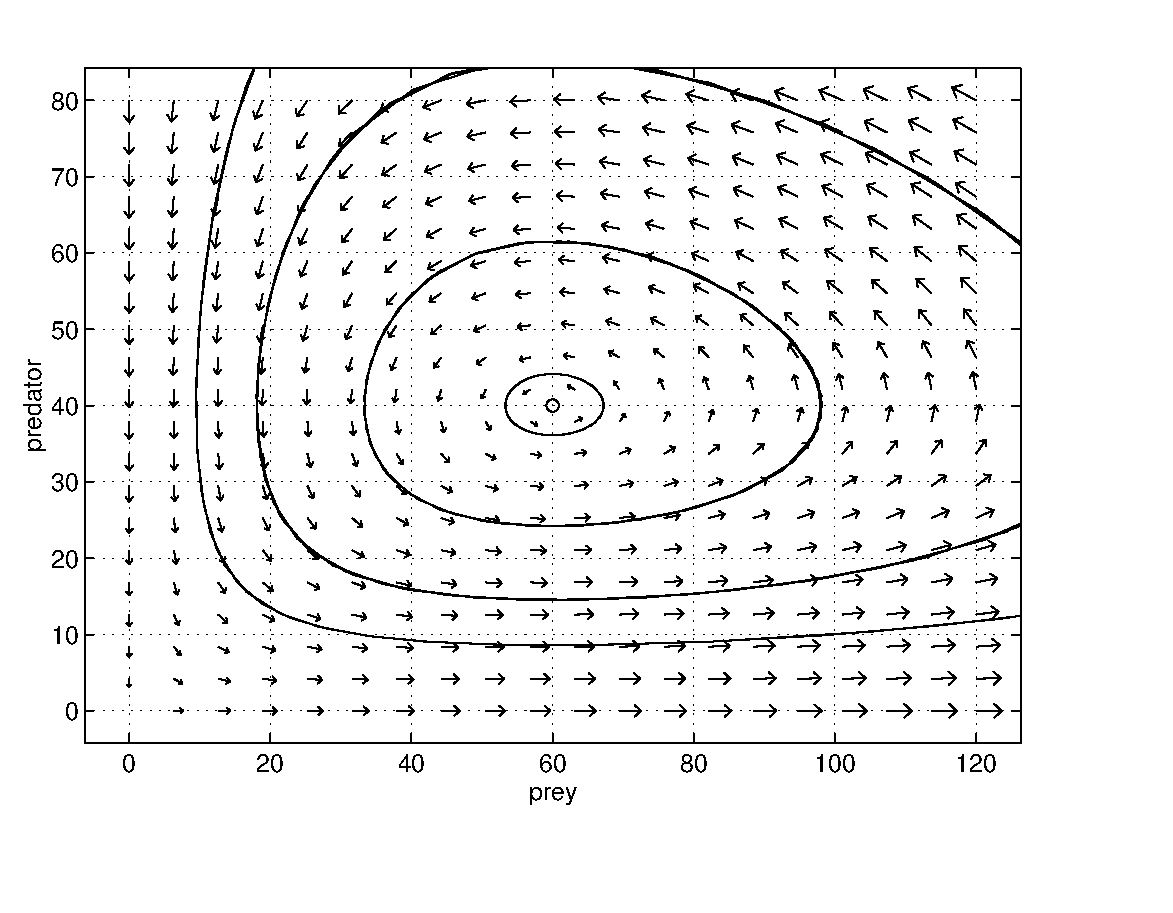
\psfig{file=figures/pp1.eps,height=3.0in}}
           \caption{Phase portrait for predator-prey equations 
		\protect\Ref{e:PP}.}
           \label{F:PP1}
\end{figure}

Note that if a solution to the predator-prey equation is time periodic, then 
the predator population and the prey population both vary periodically with 
the same period.  The assumptions (a)--(d) that went into forming the
predator-prey equations \Ref{e:PP} are reflected in the time periodic 
solutions drawn in Figure~\ref{F:PP1}.  To see this correspondence, note that 
when the predator and the prey populations are near their minimum values, then 
the prey population increases while the predator population remains nearly 
constant (assumption (a)).  After awhile, however, first the predator growth
rate and then the predator population increase (assumption (d)), and the prey 
population begins to fall (assumption (c)).  Then the prey population falls 
further and, as it does, the predator growth rate decreases (assumption (b)). 
Finally, the predator population falls until both populations are near their 
minimum values, and the whole process repeats itself exactly --- at least in
this model.  

\subsubsection*{Scaling and Reduction in the Number of Parameters}

From the discussion in Chapter~\ref{C:NPS} on Morse-Smale differential
equations, it should seem surprising that a system of nonlinear differential 
equations produces an equilibrium surrounded by a continuous family of 
periodic solutions --- just as the linear center does. \index{center} You 
might think that the values of the constants $\mu_1,\mu_2,\sigma_1,\sigma_2$ 
were chosen just so this unlikely situation would occur.  In fact, this is 
not the case as a little numerical experimentation with different values of 
$\mu_1,\mu_2,\sigma_1,\sigma_2$ will show.  

It is also surprising that a differential equation depending on four
parameters would have similar phase portraits for every one of
these parameters (assuming the appropriate sign restrictions on
the parameters).  We continue our discussion of \Ref{e:PP} by using scaling
arguments to show that three of these parameters are inessential.  

The idea behind scaling is simple.  We think of $x(t)$ as measuring the 
number of some species at time $t$.  But what is the measure?  Are we 
counting the number of individuals or the number of thousands of
individuals or even the number of millions of individuals?  For example, 
we say that the population of the United States is 275 
million people.  Similarly, when speaking of population growth, 
we choose a time unit.  Is population growth measured per year 
or per month or, in the case of bacteria, per minute?  In general, we can 
change the units of population and time without changing the type of 
solutions.  We make this change in scale by setting \index{scaling} 
\[
X(t) = \alpha x(\gamma t)  \AND  Y(t) = \beta y(\gamma t),
\]
where $\alpha,\beta,\gamma$ are positive scaling constants.  

Next, we derive differential equations for $X$ and $Y$ using the
chain rule\index{chain rule} and the differential 
equations \Ref{e:PP}. Observe that 
\[
\frac{dX}{dt}(t) = \alpha \gamma \frac{dx}{dt}(\gamma t) \AND  
\frac{dY}{dt}(t) = \beta \gamma \frac{dy}{dt}(\gamma t),
\]
and from \Ref{e:PP} that 
\begin{eqnarray*}
\frac{dX}{dt}(t) & = & \alpha \gamma \frac{dx}{dt}(\gamma t) \\
& = & \alpha \gamma x(\gamma t)(\mu_1 + \sigma_1y(\gamma t)) \\
& = & \gamma X(t)(\mu_1 + \frac{\sigma_1}{\beta}Y(t)).
\end{eqnarray*}
A similar equation holds for $\dot{Y}$.  Dropping the explicit 
dependence on $t$, we have
\begin{eqnarray*}
\frac{dX}{dt} & = & X(\gamma \mu_1 + \frac{\gamma\sigma_1}{\beta}Y)\\
\frac{dY}{dt} & = & Y(\gamma \mu_2 + \frac{\gamma\sigma_2}{\alpha}X).
\end{eqnarray*}
We now make a judicious choice of the three constants $\alpha,\beta,
\gamma$.  We choose
\begin{equation}  \label{E:scalingcoeff}
\alpha = \gamma\sigma_2, \quad \beta = -\gamma\sigma_1, \AND
\gamma = -\frac{1}{\mu_2}.
\end{equation}
These choices lead to the system of differential equations
\begin{equation*}  \label{e:PP2}
\begin{array}{lcl}
\dot{X} & = & X(\mu - Y) \\
\dot{Y} & = & Y(-1 + X),
\end{array}
\end{equation*}% \index{predator-prey equation}
where $\mu = \left|\frac{\mu_1}{\mu_2}\right|>0$.  It is easy to 
check that the scaled predator-prey equations \Ref{e:PP2} have 
an equilibrium at $(X,Y)=(1,\mu)$ that is a center.  It is also 
easy to check using {\sf pplane5} that for each $\mu$ the phase 
portrait of \Ref{e:PP2} appears to have periodic solutions 
surrounding this center.

\subsection*{The Volterra-Lotka Equations}
\index{Volterra-Lotka equations}

Next we show that if the population model \Ref{e:PP} is extended to 
a more complicated model, then the family of periodic 
solutions\index{family of periodic solutions} in 
the predator-prey equations disappears.  To understand better the 
extension that we have in mind for the predator-prey equations, we 
discuss first the single species logistic equation.
 
The {\em logistic equation\/} \index{logistic equation} is:
\[
\frac{dx}{dt} = x(\mu_1 + \rho_1x).
\]
In this model the growth rate of the population is assumed to
depend on the size of the population.  Typically, it is assumed
that the growth rate decreases as the population increases; that
is, it is assumed that $\rho_1 < 0$.  It follows that the
logistic model for two independent species is the uncoupled system:
\begin{eqnarray*}
\dot{x} & = & x(\mu_1 + \rho_1x) \\
\dot{y} & = & y(\mu_2 + \rho_2y),
\end{eqnarray*}
where $\mu_j>0,\rho_j<0$.

The {\em Volterra-Lotka\/} equations\index{Volterra-Lotka equations} 
are the simplest extension
of the uncoupled logistic system to interacting species, and
have the form:
\begin{equation} \label{e:pop2}
\begin{array}{rcl}
\dot{x} & = & x(\mu_1 +   \rho_1x + \sigma_1y) \\
\dot{y} & = & y(\mu_2 + \sigma_2x +   \rho_2y),
\end{array}
\end{equation}
where $\sigma_1,\sigma_2$ are nonzero constants.  Note that when
$\sigma_1=\sigma_2=0$ system \Ref{e:pop2} reduces to the
uncoupled logistic system. 

These equations model three different types of situations.  If
$\sigma_1>0$, then the population growth rate of the first species 
increases as the population of the second species increases.  If
$\sigma_2<0$, the population growth rate of the second species
slows as the population of the first species increases.
Suppose that the signs of $\sigma_1$ and $\sigma_2$ are
different, that is, suppose $\sigma_1<0$ and $\sigma_2>0$.  Then
the second species acts like predators (the more of the second
species there is, the lower the growth rate of the first
species), and the first species acts like prey (the more of
the first species there is, the higher the growth rate of the
second species).  In this case, the Volterra-Lotka equations are
a generalized predator-prey two species model.  Indeed,
if $\rho_1=\rho_2=0$ in \Ref{e:pop2}, then we recover the
predator-prey equations \Ref{e:PP}.  Thus, we may think of
Volterra-Lotka equations as a small perturbation of the 
predator-prey equations when $\rho_1$ and $\rho_2$ are small.
The two other cases in \Ref{e:pop2} correspond to {\em competing\/} 
species\index{competing species} ($\sigma_1,\sigma_2<0$) and 
{\em cooperating\/} species\index{cooperating species}
($\sigma_1,\sigma_2>0$).


\subsubsection*{Predator-Prey Volterra-Lotka Equations}
\index{predator-prey equation}\index{Volterra-Lotka equations}

What kind of population dynamics are predicted by equations
\Ref{e:pop2}?  The answer depends on the exact values of the 
six parameters $\mu_j,\rho_j,\sigma_j$.  As in our previous
discussion of the predator-prey equations \Ref{e:PP}, we assume
that $\mu_1>0$ and $\mu_2<0$.  To simplify the notation, we
perform the same scalings as we did when transforming \Ref{e:PP} 
to \Ref{e:PP2}, and obtain
\begin{eqnarray*} 
\dot{x} & = & x(\mu + \rho x -       y) \\
\dot{y} & = & y( -1 +       x + \eta y),
\end{eqnarray*}
where $\mu>0,\rho,\eta$ are constants.  \index{predator-prey equation}

We wish to compare the dynamics of these equations with those of 
the predator-prey model \Ref{e:PP}. To facilitate this 
comparison, we assume that $\eta=0$ and study the system of 
equations
\begin{equation*} \label{e:pop3}
\begin{array}{rcl}
\dot{x} & = & x(\mu + \rho x -       y) \\
\dot{y} & = & y( -1 +       x).
\end{array}
\end{equation*}
There is one equilibrium\index{equilibrium} where neither species 
is extinct
(that is, where $x>0$ and $y>0$).  For population dynamics the 
equilibrium $(x,y)=(1,\mu+\rho)$ is a relevant solution to 
\Ref{e:pop3} only when $\mu+\rho>0$, as we care about solutions only 
when $x\geq0, y\geq 0$.  To understand the dynamics near this
equilibrium, we compute the Jacobian matrix
\[
\mattwoc{\mu + 2\rho x-y }{-x}{y}{-1+x} = 
\mattwoc{\rho}{-1}{\mu+\rho}{0}.
\]
The determinant\index{determinant} of this matrix is $\mu+\rho>0$ and 
the trace\index{trace} is $\rho$.  Fix $\mu>0$.   It follows that for 
$\rho$ near zero and negative this equilibrium is a spiral 
sink\index{sink} and for $\rho$ near zero and positive this 
equilibrium is a spiral source\index{source}.  The
phase portraits\index{phase!portrait} for these two cases are shown in
Figure~\ref{F:pop3}.  So we see that as long as $\rho\neq 0$,
the continuous family of periodic solutions found in the simpler
predator-prey equations \Ref{e:PP} disappears.\index{periodic solution}


\begin{figure}[htb]
           \centerline{%
	   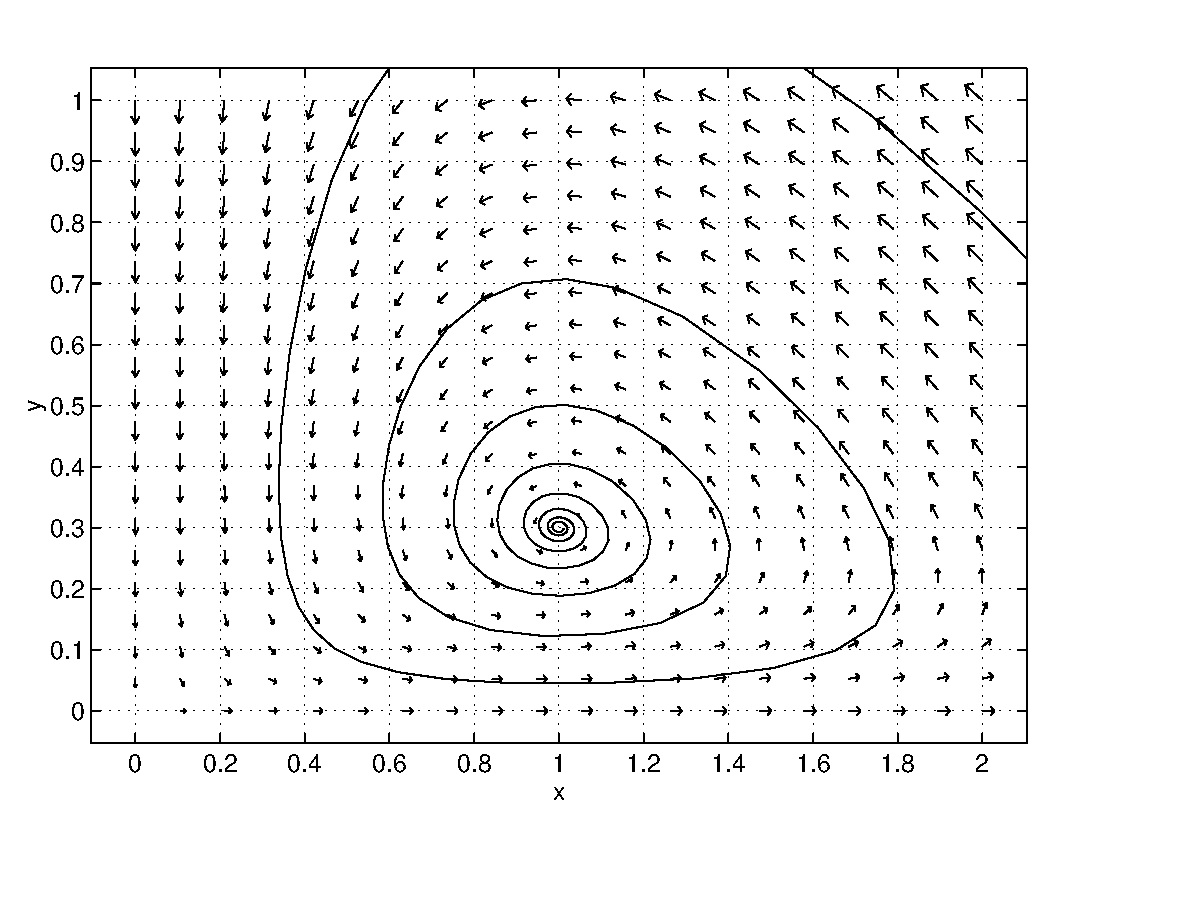
\psfig{file=figures/pop3a.eps,height=2.5in}
	   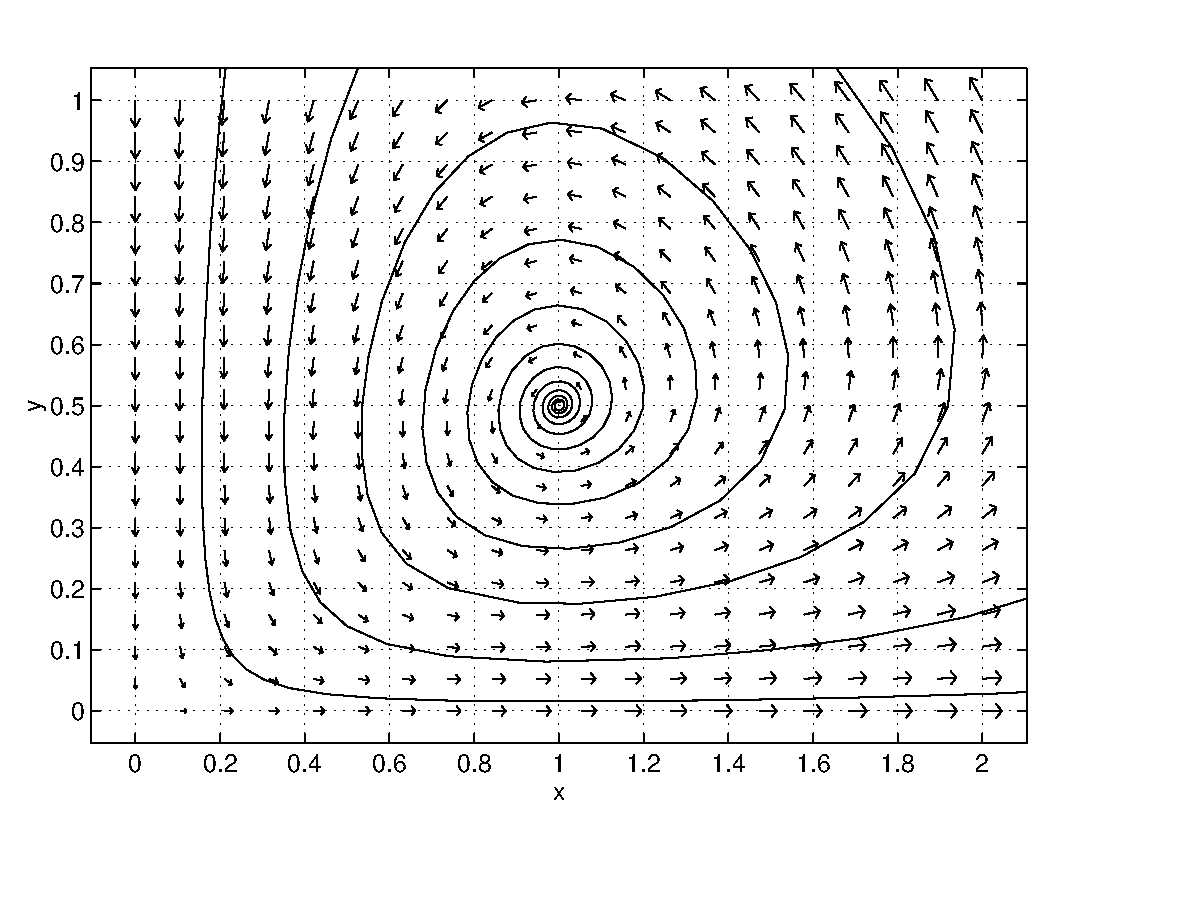
\psfig{file=figures/pop3b.eps,height=2.5in}}
		\vspace*{-0.2in}		
		\hspace{1.0in} $\rho=-0.1$ \hspace{2.5in} $\rho=0.1$
           \caption{Phase portraits for Volterra-Lotka predator-prey 
		equations \protect\Ref{e:pop3} with $\mu=0.4$.}
           \label{F:pop3}
\end{figure}

\EXER

\TEXER

\begin{exercise} \label{c9.1.5}
Consider the two predator-prey equations
\begin{equation} \label{E:prpr1}
\begin{array}{rcl}
\dot{x} & = & x(2-10y)\\
\dot{y} & = & y(-4+y)
\end{array}
\end{equation}
and 
\begin{equation} \label{E:prpr2}
\begin{array}{rcl}
\dot{x} & = & x(2-0.1y)\\
\dot{y} & = & y(-4+y)
\end{array}
\end{equation}
In one of these equations the predators eat the prey 100 times more 
frequently than in the other.  Which one?
\end{exercise}

\begin{exercise} \label{c9.1.6}
Show that the predator-prey equations \Ref{E:prpr1} and \Ref{E:prpr2} both 
scale to the same equation \Ref{e:PP2}.  For each equation what are the 
values of the scaling coefficients $\alpha,\beta,\gamma$ defined in 
\Ref{E:scalingcoeff}?  What is the common value of $\mu$?
\end{exercise}



\begin{exercise} \label{c9.1.2}
Consider the following special case of the Volterra-Lotka equations 
\begin{eqnarray*}
\dot{x} & = & x(\mu + 2x -     y)  \\
\dot{y} & = & y(  1 +  x - 0.25y).
\end{eqnarray*}
For what value of $\mu$ is there an equilibrium whose linearization is a 
center?   
\end{exercise}

\begin{exercise} \label{c9.1.1}
Consider the Volterra-Lotka equations when $\mu_1,\mu_2>0$, 
$\rho_1,\rho_2 < 0$, and $\sigma_1<0,\sigma_2>0$. Scaling these 
equations leads to the system
\begin{equation*}
\begin{array}{rcl}
\dot{x} & = & x(\mu + \rho x -         y)  \\
\dot{y} & = & y(  1 +        x +  \eta y),
\end{array}
\end{equation*}
where $\mu>0$ and $\rho,\eta<0$.  
\begin{itemize}
\item[(a)]  There are four possible equilibria depending on whether $x$ and 
$y$ vanish or not.  Find these equilibria and their type (saddle, sink, 
source or nonhyperbolic).  {\bf Hint:} Use the equations for the equilibrium 
where both coordinates are nonzero 
\[
\mu + \rho x - y = 0 \AND  1 + x +  \eta y = 0
\]
to show that the Jacobian matrix at that equilibrium is:
\[
(df) =\mattwoc{\rho x}{-x}{y}{\eta y}.
\]
\item[(b)]  Set $\rho=-1.5$ and $\eta=-1$ and discuss the phase portraits 
of these equations for different values of $\mu$.  Verify your answer 
using {\sf pplane5}. 
\end{itemize}
\end{exercise}



\CEXER

\begin{exercise} \label{c9.1.3}
Choose values for the constants in the predator-prey equations 
\Ref{e:PP} and verify numerically that there is a unique 
equilibrium surrounded by periodic solutions in the first 
quadrant of the phase portrait for these equations.
\end{exercise}

\begin{exercise} \label{c9.1.4}
Choose values for the constants in the Volterra-Lotka predator-prey equations 
\Ref{e:pop3} and verify numerically that there are no periodic solutions in 
the first quadrant for these equations.
\end{exercise}

\begin{exercise} \label{c9.1.7}
Use {\sf pplane5} to describe the (numerical) differences between solutions 
to the differential equations \Ref{E:prpr1} and \Ref{E:prpr2}.  In particular,
compare the maximum number of prey in one equation with the maximum number of 
prey in the other equation when you start with the same number of predators 
and prey in each equation.
\end{exercise}

\begin{exercise} \label{c9.1.8}
Foxes (the predators) and rabbits (the prey) coexist in an isolated area.
In equilibrium, there are 200 foxes and 10,000 rabbits.  When isolated from
the foxes, the rabbit population doubles every year.  When isolated from 
the rabbits, the fox population decreases at the rate of 10\% per year. 
Supposing that the fox-rabbit populations are modeled by the predator-prey
equations \Ref{e:PP}, answer the following questions.
\begin{itemize}
\item[(a)]  	What are the values of $\mu_1,\mu_2,\sigma_1,\sigma_2$ in 
\Ref{e:PP}.
\item[(b)]	After a storm 1,200 rabbits and 110 foxes remain in the area.
According to this model, what will the fox population be after three years?  
{\bf Hint:}  Use the {\sf Specify a computation interval} on the 
{\sf PPLANE5 Keyboard input} menu.
\item[(c)]	After the storm, what is the maximum number of rabbits that 
this model predicts will inhabit the area.
\item[(d)]	How many years will it take the rabbit population to reach 
this maximum number for the first time?
\end{itemize}
\end{exercise}


\section{Examples of Bifurcations}
\label{S:bifurcation} \index{bifurcation}

In Section~\ref{S:TSPM} we illustrated how modeling leads to systems 
of differential equations that depend on external parameters.  In this 
section we discuss some of the expected ways in which phase portraits of 
systems of differential equations change as a single parameter is varied.  
These ways include changes in the number of equilibria and in the number 
of limit cycles, and are called {\em bifurcations\/}.   We use simple 
differential equations to illustrate three different kinds of bifurcation: 
{\em saddle-node\/} bifurcations where two equilibria collide and disappear; 
{\em Hopf\/} bifurcations where limit cycles are created; and 
{\em homoclinic\/} bifurcations where limit cycles disappear.  We also show 
how to use {\em bifurcation diagrams\/} to summarize these changes.

\subsection*{Saddle-Node Bifurcations on the Line}
\index{bifurcation!saddle-node}

Consider the differential equation
\begin{equation}  \label{E:sbif}
\dot{x} = \rho - x^2 \equiv f(x,\rho).
\end{equation}
We discuss how the phase line to \Ref{E:sbif} changes as $\rho$ increases 
through $0$.  A simple numerical experiment using {\sf pline} shows that
the phase lines for \Ref{E:sbif} when $\rho=-1,0,1$ are those given in 
Figure~\ref{F:sbif}.  From this figure we see that a pair of equilibria 
is created as $\rho$ increases through $0$.

\vspace{0.4in}

\begin{figure}[htb]
           \centerline{%
           \psfig{file=figures/sbif.eps,width=6.0in}}
           \caption{Phase lines for the differential equation 
    		\protect\Ref{E:sbif}.}
           \label{F:sbif}
\end{figure}\index{phase!line}


These phase lines can be verified analytically by solving the 
algebraic equation $f(x,\rho)=0$ and obtaining:
\begin{equation} \label{E:sbife}
x^2 = \rho.
\end{equation}
When $\rho<0$ there are no (real) solutions to \Ref{E:sbife}; when
$\rho=0$ the only solution to \Ref{E:sbife} is $x=0$; and when $\rho>0$
there are two solutions to \Ref{E:sbife} given by $x=\pm\sqrt{\rho}$.
It follows that \Ref{E:sbif} has no equilibria when $\rho<0$, a single
equilibrium when $\rho=0$, and two equilibria when $\rho>0$.

Additionally, we can determine the stability\index{stability}
of the equilibria using 
Theorem~\ref{T:stability1} in Chapter~\ref{chap:SolveOdes}.  Observe that
\[
f_x(x,\rho) = -2x.
\]
Therefore, $f_x<0$ at $x=\sqrt{\rho}$ and $f_x>0$ at $x=-\sqrt{\rho}$.
Theorem~\ref{T:stability1} implies that the equilibrium at $x=-\sqrt{\rho}$ 
is unstable and that the equilibrium at $x=\sqrt{\rho}$ is stable.

We summarize the information about equilibria of \Ref{E:sbif} in the 
bifurcation diagram\index{diagram!bifurcation} in Figure~\ref{F:sbifBIF}.  
This bifurcation diagram is formed as follows: graph the points where 
$f(x,\rho)=0$ in the $\rho x$ plane; that is, graph the parabola $\rho=x^2$.  
On that graph we use a solid line when the equilibrium of \Ref{E:sbif} is 
stable and a dashed line when the equilibrium is unstable.

\begin{figure}[htb]
           \centerline{%
           \psfig{file=figures/sbifBIF.eps,width=4.0in}}
           \caption{Bifurcation diagram for the differential equation
        \protect\Ref{E:sbif}. }
           \label{F:sbifBIF}
\end{figure}

We have shown that at $\rho=0$ the differential equation \Ref{E:sbif} 
undergoes a saddle-node bifurcation\index{bifurcation!saddle-node}
where a pair of equilibria is created.  Moreover, one of this pair is stable 
and one is unstable.  Next, we consider a more complicated example:
\begin{equation} \label{E:cbif}
\dot{x} = \rho - x^3 + 3x \equiv f(x,\rho).
\end{equation}
We can solve for the equilibria of this differential equation by solving
the algebraic equation $f(x,\rho)=0$ for
\begin{equation}  \label{E:rho=cubic}
\rho = x^3 - 3x.
\end{equation}
Graphing \Ref{E:rho=cubic} in the $\rho x$ plane yields the bifurcation 
diagram in Figure~\ref{F:cbifBIF}.  Note that two equilibria appear at 
$\rho=-2$ as $\rho$ increases and that two equilibria disappear at 
$\rho=2$.  Thus, there are two saddle-node bifurcations for \Ref{E:cbif}: 
one at $\rho=-2$ and one at $\rho=2$.

\begin{figure}[htb]
           \centerline{%
           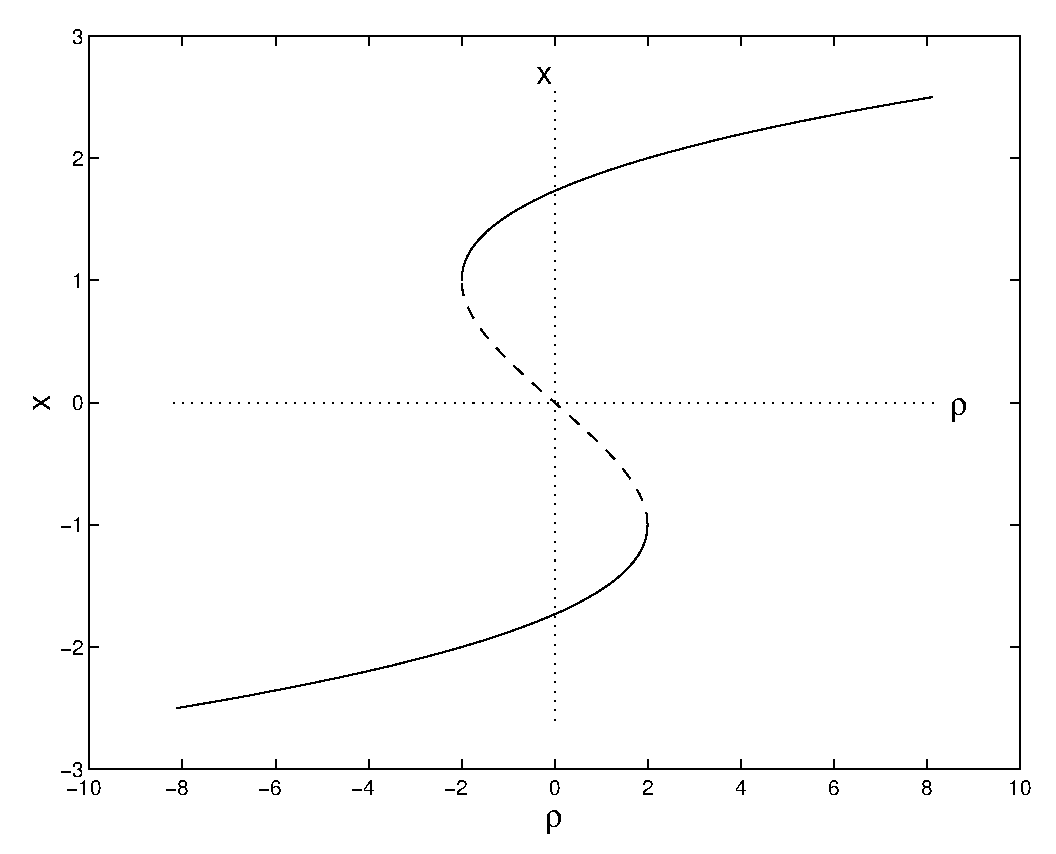
\psfig{file=figures/cbifBIF.eps,width=4.0in}}
           \caption{Bifurcation diagram for the differential equation
        \protect\Ref{E:cbif}.}
           \label{F:cbifBIF}
\end{figure} \index{diagram!bifurcation}

In Figure~\ref{F:cbifBIF} we have again plotted stable equilibria
\index{equilibrium!stable} using solid lines and unstable equilibria
\index{equilibrium!unstable} using dashed lines.  The
stability can be checked analytically by computing
\[
f_x(x,\rho) = -3x^2+3 = 3(1-x^2).
\]
It follows that $f_x<0$ at equilibria where $|x|>1$ and $f_x>0$ at 
equilibria where $|x|<1$.  So the equilibria at $x$ values between 
$-1$ and $1$ are unstable and the equilibria at $x>1$ and $x<-1$ are 
stable.  The phase lines are those given in Figure~\ref{F:cbif}.  These 
calculations can be verified using {\sf pline}. 

\vspace{0.4in}

\begin{figure}[htb]
           \centerline{%
           \psfig{file=figures/cbif.eps,width=6.0in}}
           \caption{Phase lines for the differential equation
        \protect\Ref{E:cbif}.}
           \label{F:cbif}
\end{figure}

\subsubsection*{The Detection of 1-D Saddle-Node Bifurcations}

In differential equations of the form
\[
\dot{x} = f(x,\rho)
\]
we have seen that at points $(x_0,\rho_0)$ where saddle-node bifurcations
occur two equilibria collide as the parameter $\rho$ is varied, and one of 
these equilibria is stable while the other one is unstable.  Therefore, the
following restrictions on $f$ must hold:
\begin{equation}  \label{E:DCSN}
\begin{array}{rcl}
f(x_0,\rho_0) & = & 0\\
f_x(x_0,\rho_0) & = & 0.
\end{array}
\end{equation}
The first condition just states that the point $(x_0,\rho_0)$ is an
equilibrium of the differential equation.  The second condition follows from
continuity; there are two equilibria nearby one of which is asymptotically 
stable $f_x<0$ and the other is unstable $f_x>0$.  In between, which means at
the point $(x_0,\rho_0)$, we must have $f_x=0$.

For example, we can find points where saddle-node bifurcations might occur in 
the differential equation:
\[
\dot{x} = 2x^2 +\rho x + 2
\]
by solving the two equations given in \Ref{E:DCSN}.  Set 
\[
f(x,\rho) = 2x^2 +\rho x + 2
\]
and differentiate to obtain
\[
f_x(x,\rho) = 4x + \rho.
\]
On setting $f_x=0$ we find
\[
\rho = -4x.
\]
Substituting this result into the equation $f=0$ yields
\[
-2x^2 + 2 =0
\]
which can be solved for $x=\pm 1$.  There are two possible points where
saddle-node bifurcations can occur; they are:
\[
(x_0,\rho_0) = (1,-4) \AND  (x_0,\rho_0) = (-1,4).
\]
It can be checked using {\sf pline} that saddle-node bifurcations do actually
occur at both points.

Conditions \Ref{E:DCSN} are necessary conditions for the existence of a 
saddle-node bifurcation; by themselves they are not sufficient.  For example, 
consider
\[
f(x,\rho) = x^2 -\rho^2.
\]
Since $f(0,0)=0$ and $f_x(0,0)=0$, the origin satisfies \Ref{E:DCSN}.  But 
the bifurcation is not a saddle-node bifurcation as there 
are two equilibria for every nonzero value of $\rho$.

\subsection*{Saddle-Node Bifurcations in the Plane}
\index{bifurcation!saddle-node!in the plane}

The transition from no equilibria to two equilibria can occur as a 
parameter is varied in differential equations with any number of 
variables.  Here we consider one example of a planar system of 
differential equations where a saddle-node bifurcation occurs.
Consider the system of differential equations 
\begin{equation*}  \label{E:ssys}
\begin{array}{rcl}
\dot{x} & = & x^2 - \rho + y \\
\dot{y} & = & -y(x^2+1).  \end{array}
\end{equation*}

From the $\dot{y}$ equation we see that equilibria only occur 
when $y=0$.  Substituting $y=0$ into the $\dot{x}$ equation yields
the equation $x^2=\rho$.   Thus there are no equilibria for $\rho<0$;
a single equilibrium at the origin for $\rho=0$; and two equilibria
at 
\[
X_{\pm}=(\pm\sqrt{\rho},0)
\]
for $\rho>0$.  The bifurcation diagram 
for the system of differential equations \Ref{E:ssys} is identical to
the one for the single equation \Ref{E:sbif} given in Figure~\ref{F:sbif}.

In Figure~\ref{F:ssys}, the phase portraits of \Ref{E:ssys} are given for 
two values of $\rho$; namely, $\rho=-1$ and $\rho=1$.  Note that when 
$\rho=0$ the origin is a nonhyperbolic 
equilibrium\index{equilibrium!nonhyperbolic} and when $\rho=1$
the equilibrium at $(-1,0)$ is a nodal sink\index{nodal sink} 
while the equilibrium at 
$(1,0)$ is a saddle\index{saddle}.  
Thus this saddle-node bifurcation creates a saddle 
and a nodal sink.  In all planar saddle-node bifurcations one of the 
equilibria will be a saddle and the other will either be a nodal source 
or a nodal sink.  See Exercise~\ref{e:source}.

\begin{figure}[htb]
           \centerline{%
           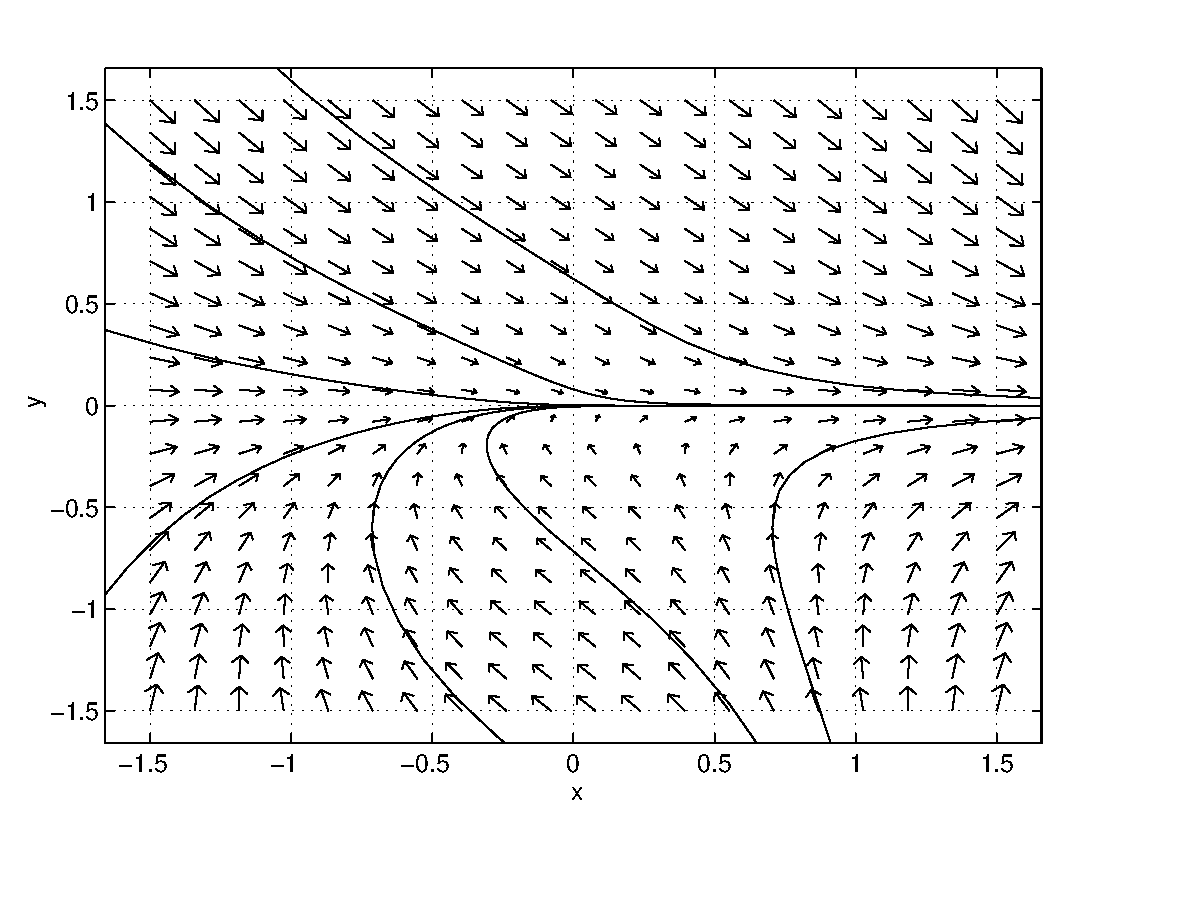
\psfig{file=figures/ssys1.eps,height=2.0in}
	   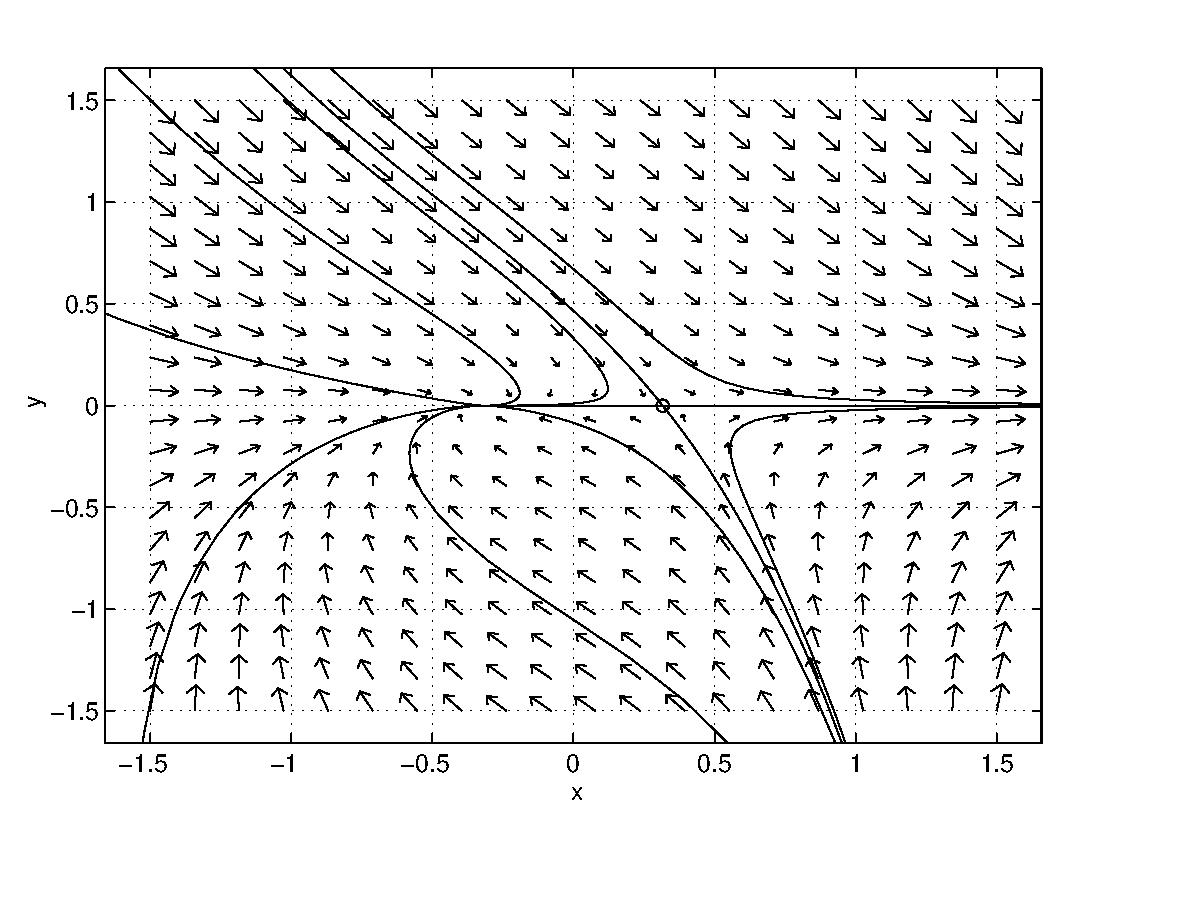
\psfig{file=figures/ssys3.eps,height=2.0in}}
		\vspace*{-0.2in}		
		\hspace{1.3in} $\rho=-1$ \hspace{2.1in} $\rho=1$
   \caption{Phase planes for the differential equation \protect\Ref{E:ssys}.}
           \label{F:ssys}
\end{figure}

It is instructive to determine the type of equilibria in \Ref{E:ssys} by
computing the Jacobian matrix.  Let $F(x,y)$ denote the right hand side of 
\Ref{E:ssys} and calculate:
\begin{equation}  \label{E:SNJ}
dF = \mattwoc{2x}{1}{-2xy}{-x^2-1} \AND 
(dF)_{X_{\pm}}= \mattwoc{\pm 2\sqrt{\rho}}{1}{0}{-\rho-1}.
\end{equation}
Observe that when $\rho=0$ the linearized differential equation, at the origin, 
is the nonhyperbolic saddle-node
\[
\dot{X} = \mattwo{0}{1}{0}{-1}X,
\]
whose eigenvalues are $0$ and $1$.  See Section~\ref{S:6.9}. We can also check
using \Ref{E:SNJ} that when $\rho>0$ the linearization at $X_{-}$ has two 
negative real eigenvalues ($-2\sqrt{\rho}$ and $-\rho-1$)  and is a node 
while the linearization at $X_{+}$ has one positive ($2\sqrt{\rho}$) and one 
negative ($-\rho-1$) eigenvalue and is a saddle.


\subsubsection*{Detection of 2D Saddle-Node Bifurcations}

Saddle-node bifurcations occur in planar systems at equilibria  where a 
saddle and a node coalesce.  Consider the planar system of differential 
equations
\[
\dot{X} = F(X,\rho).
\]
At a saddle-node bifurcation point $(X_0,\rho_0)$, the following conditions
must be satisfied:
\begin{equation}  \label{E:DCSN2}
\begin{array}{rcl}
F(X_0,\rho_0) & = & 0\\
\det(J) & = & 0.
\end{array}
\end{equation}
where $J = (dF)_{(X_0,\rho_0)}$ satisfies $\trace(J)\neq 0$.  The first 
equation just states that $(X_0,\rho_0)$ is an equilibrium and the second 
equation implies that the Jacobian has a zero eigenvalue.  Since 
$\trace(J)\neq 0$, $J$ has a nonzero eigenvalue and is a saddle-node matrix.

We can use \Ref{E:DCSN2} to find possible saddle-node bifurcation points in
planar systems.  For example, consider the system
\[
\begin{array}{rcl} 
\dot{x} & = & x^2 + y^2 - \rho\\
\dot{y} & = & x + y -2.
\end{array}
\]
The two parts of \Ref{E:DCSN2} lead to three equations:
\[
\begin{array}{rcl} 
x^2 + y^2 - \rho & = & 0\\
x + y -2 & = 0\\
\det\mattwoc{2x}{2y}{1}{1} & = & 0.
\end{array}
\]
These equations can be solved for $(x_0,y_0,\rho_0)=(1,1,2)$.  Indeed, for 
$\rho\approx 2$, {\sf pplane5} can be used to show that there are two 
equilibria near $(1,1)$ (a saddle and a node) when $\rho>2$ and no 
equilibria near $(1,1)$ when $\rho<2$.



\subsection*{Hopf Bifurcation in a Planar System} 
\index{bifurcation!Hopf}

Another type of bifurcation that can occur in planar systems (though not in
single autonomous equations) is the creation of a limit cycle from an
equilibrium.  This type of bifurcation is commonly called {\em Hopf 
bifurcation\/}.  We begin our discussion with a numerical example.  

Load the planar system of differential equations 
\begin{equation*} \label{E:Hopfbif}
\begin{array}{rcl}
\dot{x} & = & y \\
\dot{y} & = & -x + \rho y - y^3  \end{array}
\end{equation*}
into {\sf pplane5}.
It is straightforward to see that the origin is an equilibrium of 
\Ref{E:Hopfbif} for all values of $\rho$ --- indeed, the origin is 
the only equilibrium of \Ref{E:Hopfbif}.  Now plot the phase 
portraits for $\rho=-1$ and $\rho=1$.  These plots are shown in 
Figure~\ref{F:Hopfbif}.  

\begin{figure}[htb]
           \centerline{%
           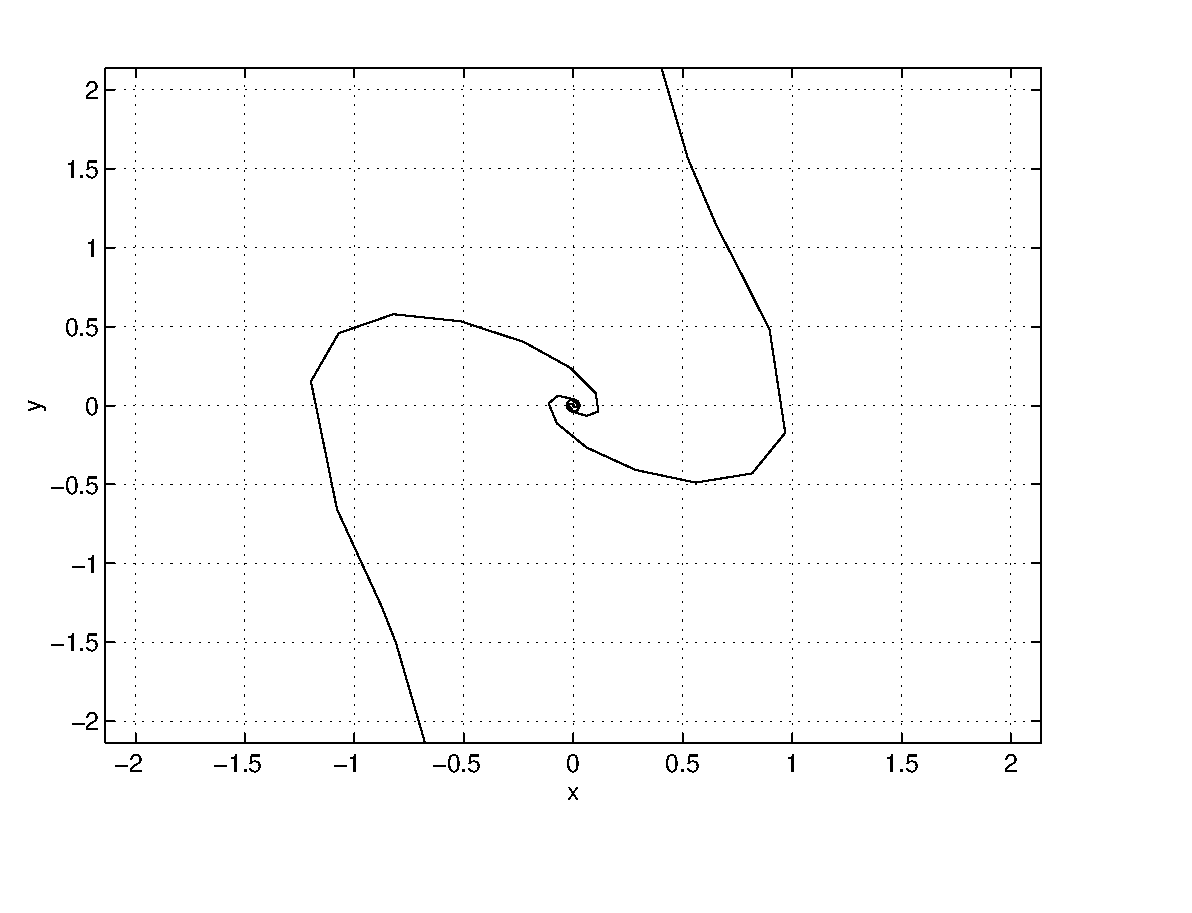
\psfig{file=figures/Hopfbif1.eps,height=2.5in}
           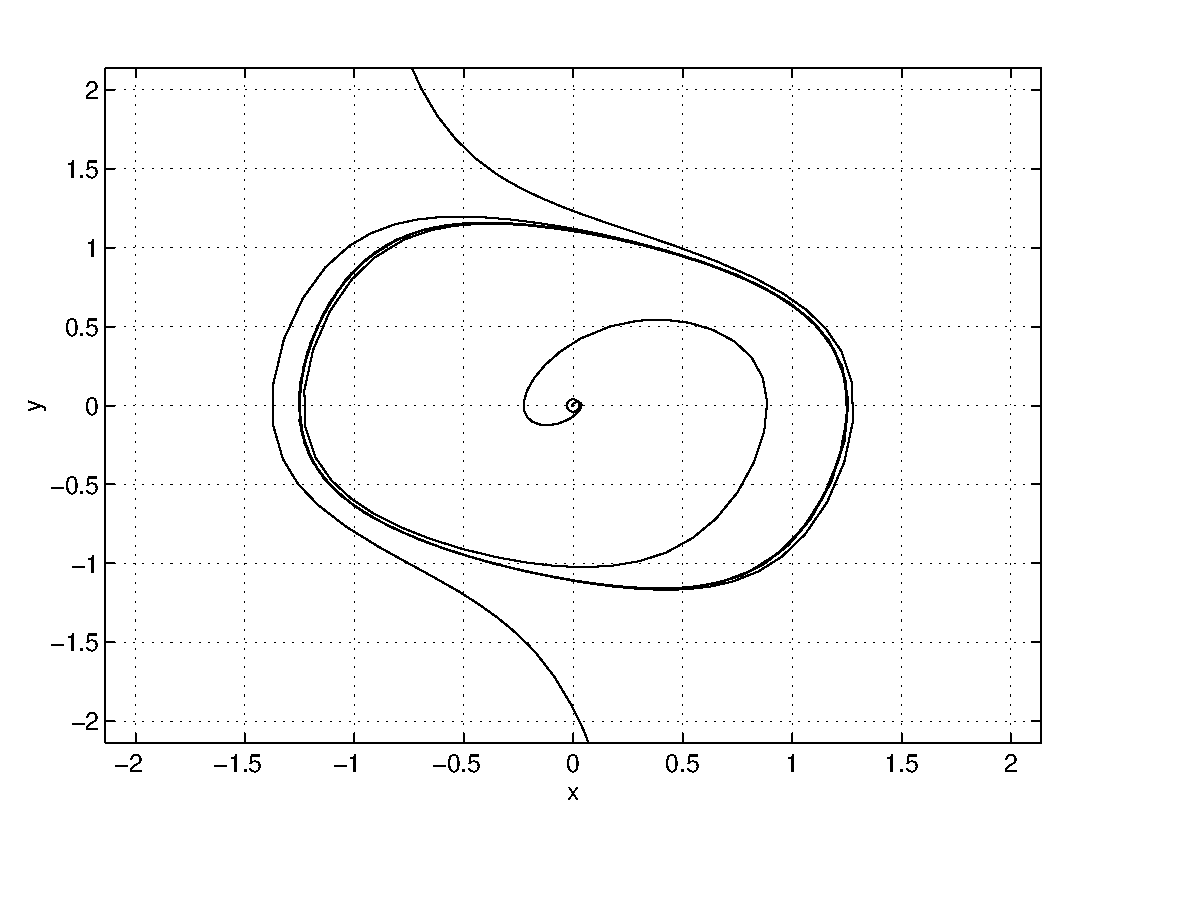
\psfig{file=figures/Hopfbif2.eps,height=2.5in}}
		\vspace*{-0.2in}		
		\qquad\qquad\qquad $\rho=-1$ \hspace{2.8in} $\rho=1$
	   \caption{Phase planes for the differential equation 
      \protect\Ref{E:Hopfbif}.}
           \label{F:Hopfbif}
\end{figure}


The Jacobian of \Ref{E:Hopfbif} at the origin is:
\[
\mattwoc{0}{1}{-1}{\rho}.
\]
It follows that the origin goes from being a 
spiral sink\index{sink} to being a 
spiral source\index{source} 
as $\rho$ increases through $0$.  It also follows that  
the origin is a center\index{center} at $\rho=0$.  
The main new feature of the phase portraits is the 
existence of an asymptotically stable\index{stability!asymptotic} 
periodic solution when $\rho>0$.  
Hopf bifurcations can also produce unstable periodic solutions
\index{periodic solution!unstable} (see \Ref{E:hopfdetect} for an example).   

\subsubsection*{Bifurcation Diagrams for Hopf Bifurcation}

There are two salient points concerning Hopf bifurcation.  The first point is 
that a spiral sink equilibrium loses stability and becomes a spiral source 
as a parameter is varied (or vice versa).  The second point is that a limit
cycle (either stable or unstable) is produced by this change in stability. 
We draw schematic bifurcation diagrams in
Figures~\ref{F:Hopfbifdiag}--\ref{F:Hopfbifdiag2} to indicate this change.  
On this diagram stable equilibria are indicated by a 
solid line and unstable equilibria are indicated by a dashed line, as before.
Stable limit cycles are indicated by a heavy dotted line and unstable limit 
cycles are indicated by a dot-dashed line.  Note that the bifurcation diagram
in Figure~\ref{F:Hopfbifdiag} describes the Hopf bifurcation in the system of
differential equations \Ref{E:Hopfbif}. 

\begin{figure}[htb]
           \centerline{%
           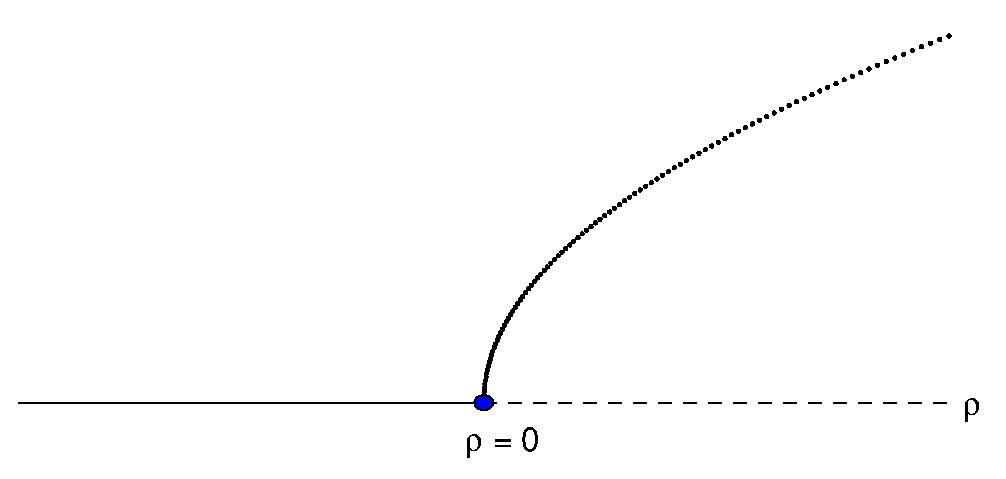
\psfig{file=figures/Hopfbifa.eps,height=1.6in}}
  \caption{Schematic bifurcation diagram for the differential equation 
    \protect\Ref{E:Hopfbif} with a branch of stable limit cycles emanating 
	from a point of Hopf bifurcation indicated by a dotted line.}
           \label{F:Hopfbifdiag}
\end{figure}
\index{diagram!bifurcation}

\begin{figure}[htb]
           \centerline{%
           \psfig{file=figures/Hopfbifb.eps,height=1.6in}}
  \caption{Schematic bifurcation diagram with a branch of unstable limit 
	cycles emanating from a point of Hopf bifurcation indicated by a 
	dot-dashed line.}
           \label{F:Hopfbifdiag2}
\end{figure}
\index{diagram!bifurcation}

\subsubsection*{Detection of Hopf Bifurcations}

A necessary condition for producing a limit cycle from an equilibrium by
varying an external parameter is the existence of an equilibrium whose
linearization is a center.  Thus, $(X_0,\rho_0)$ is a possible point of 
Hopf bifurcation for the planar system
\[
\dot{X} = F(X,\rho)
\]
if the following conditions are satisfied:
\begin{equation} \label{E:NCHB}
\begin{array}{rcl}
F(X_0,\rho_0) & = & 0\\
\trace(J) & = & 0\\
\det(J) & > & 0
\end{array}
\end{equation}
where $J= (dF)_{(X_0,\rho_0)}$.

We can use \Ref{E:NCHB} to find possible points of Hopf bifurcation.  For 
example, consider the system
\begin{equation*}  \label{E:hopfdetect}
\begin{array}{rcl}
\dot{x} & = & 2y - \rho + x^2 - 2y^2\\
\dot{y} & = & -x + y^2.
\end{array}
\end{equation*}
A point of Hopf bifurcation in \Ref{E:hopfdetect} must satisfy the three 
equations
\[
\begin{array}{rcl}
2y - \rho  + x^2 - 2y^2 & = & 0\\
-x + y^2 & = & 0 \\
2(x + y)  & = & 0,
\end{array}
\]
where, in addition, $\det(J) = 4xy+2-4y>0$.  It follows from the third 
equation ($\trace(J)=0$) that $y=-x$.  On substitution for $y$ in the first 
two equations, we find
\[
\begin{array}{rcl}
-2x - \rho - x^2 & = & 0\\
-x + x^2 & = & 0,
\end{array}
\]
where $\det(J) = -4x^2+4x+2$.  From the second equation it follows that $x=0$
or $x=1$.  So there are two solutions to this system of equations: 
$(x_0,y_0,\rho_0)=(0,0,0)$ and $(x_1,y_1,\rho_1)=(1,-1,-3)$.  At both of
these points the determinant of the Jacobian matrix is $2$.  Hence the
linearized equations at both point are centers, and there are two possible
points of Hopf bifurcation.

Numerical exploration of \Ref{E:hopfdetect} using {\sf pplane5} shows that 
there are unstable limit cycles emanating from both of these points; hence 
there are exactly two points of Hopf bifurcation in this system of equations.



\subsection*{Conventions for Bifurcation Diagrams}

In all bifurcation diagrams we will indicate
\begin{itemize}
\item	stable equilibria by a solid line;
\item	unstable equilibria by a dashed line;
\item	stable limit cycles by a dotted line;
\item	unstable limit cycles by a dot-dashed line; and
\item	bifurcation points by black circles.
\end{itemize}

For example, the information contained in the Hopf bifurcation of 
\Ref{E:Hopfbif} is summarized by the bifurcation diagram in 
Figure~\ref{F:Hopfbifdiag}.
In that figure, a curve of equilibria \index{curve of equilibria} 
loses stability at $\rho=0$ as $\rho$ increases.  A branch of limit 
cycles\index{limit cycle!branch of} emanates from the
branch of equilibria at the bifurcation point, which is indicated by a 
black dot.  The stable limit cycles are indicated by the dotted line.



\subsection*{Homoclinic Bifurcations}
\index{bifurcation!homoclinic}

There is a second way that planar systems of differential equations 
can have periodic solutions appear or disappear as parameters are varied.  
This  change is called a {\em homoclinic bifurcation\/}.  For example,
consider the system of differential equations
\begin{equation*}  \label{E:homobif}
\begin{array}{rcl} 
\dot{x} & = & \rho x - y \\
\dot{y} & = &  x + x^2 + xy.
\end{array}
\end{equation*}
Begin by noting that the origin is an equilibrium of \Ref{E:homobif}
for every value of $\rho$ and the linearized equation about this equilibrium 
is:
\[
\dot{X} = \mattwo{\rho}{-1}{1}{0}X.
\]
It follows that \Ref{E:homobif} has a Hopf bifurcation at the origin, as 
the origin changes from a spiral sink to a spiral source as $\rho$ 
increases through zero.  Calculations show that \Ref{E:homobif} has a 
second equilibrium at 
\[
X_0 = -\frac{1}{1+\rho}(1,\rho)
\]
and that this equilibrium is a saddle when $\rho>-1$.

\begin{figure}[htb]
           \centerline{%
           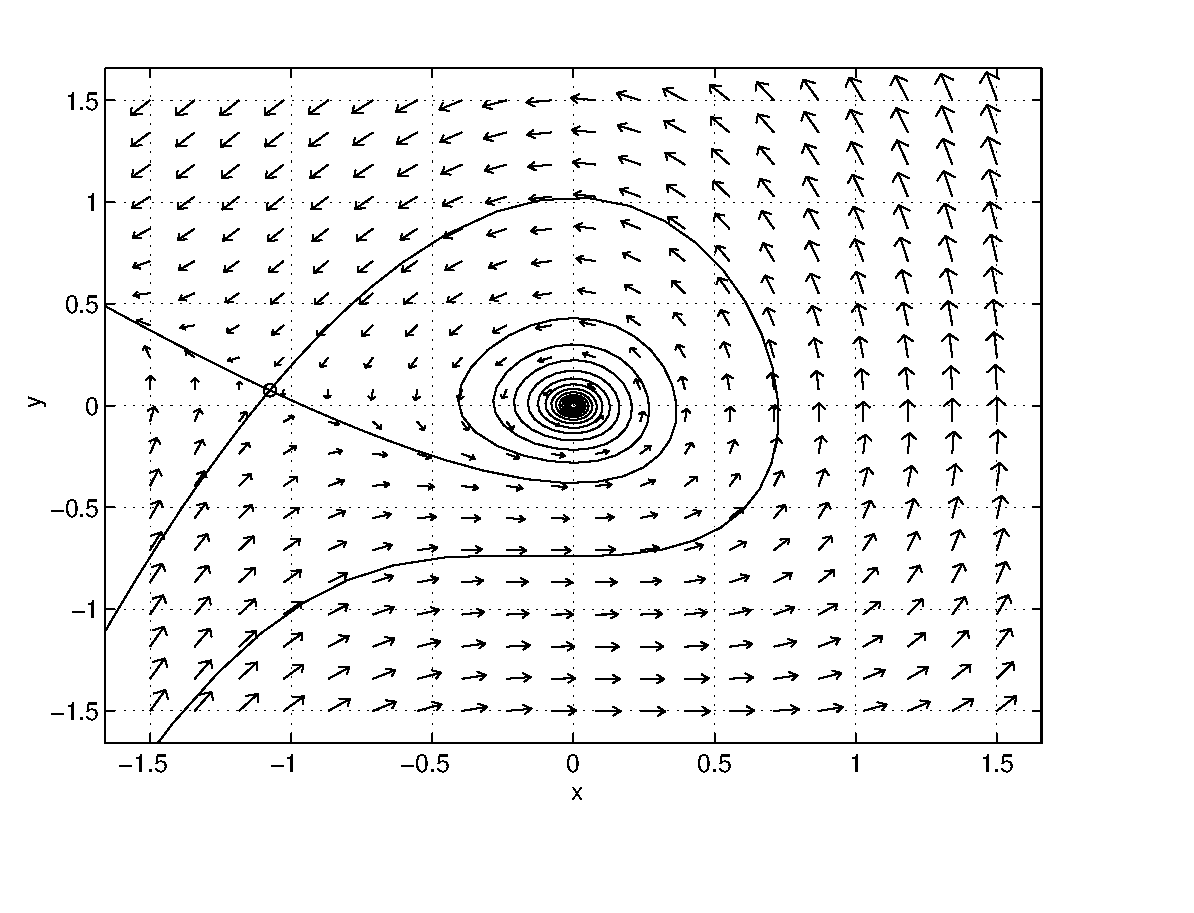
\psfig{file=figures/homobif1.eps,height=2.0in}
           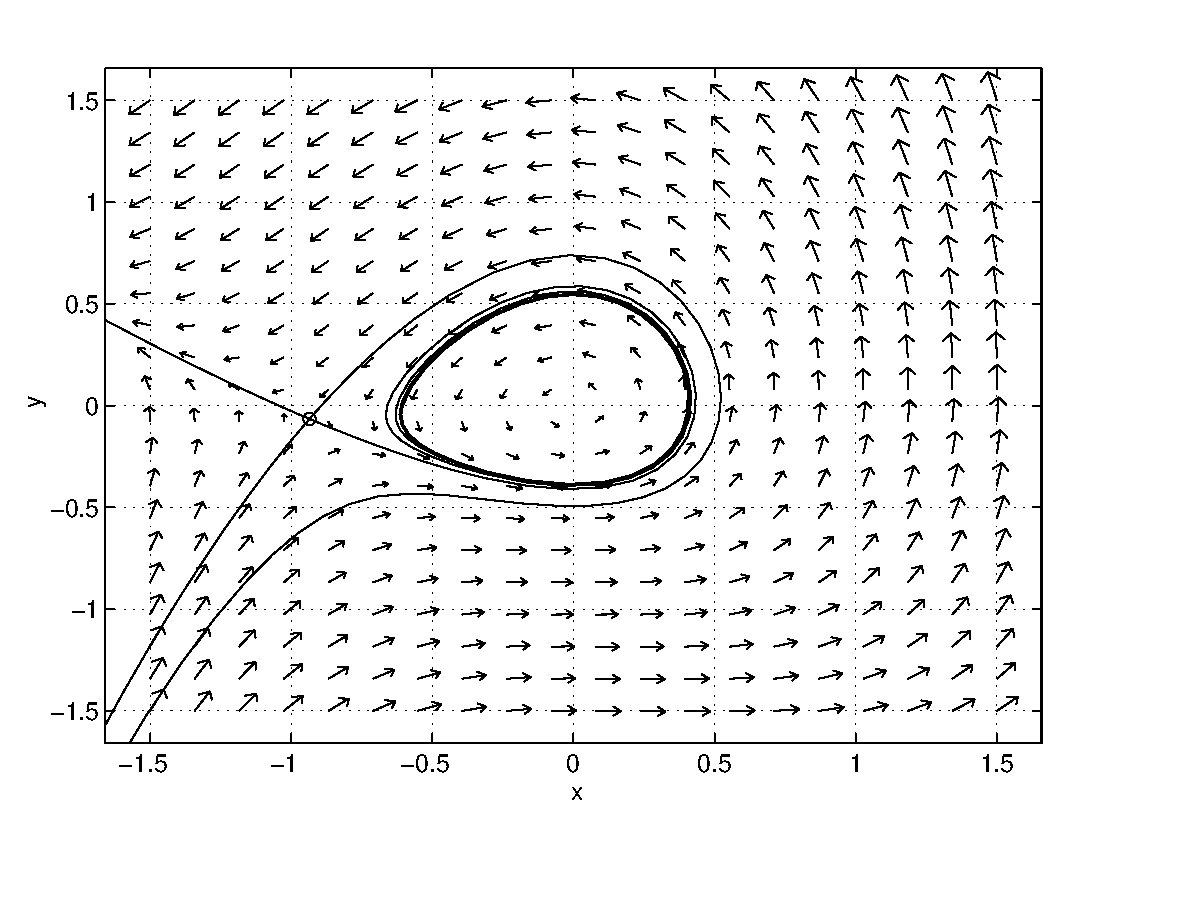
\psfig{file=figures/homobif2.eps,height=2.0in}
           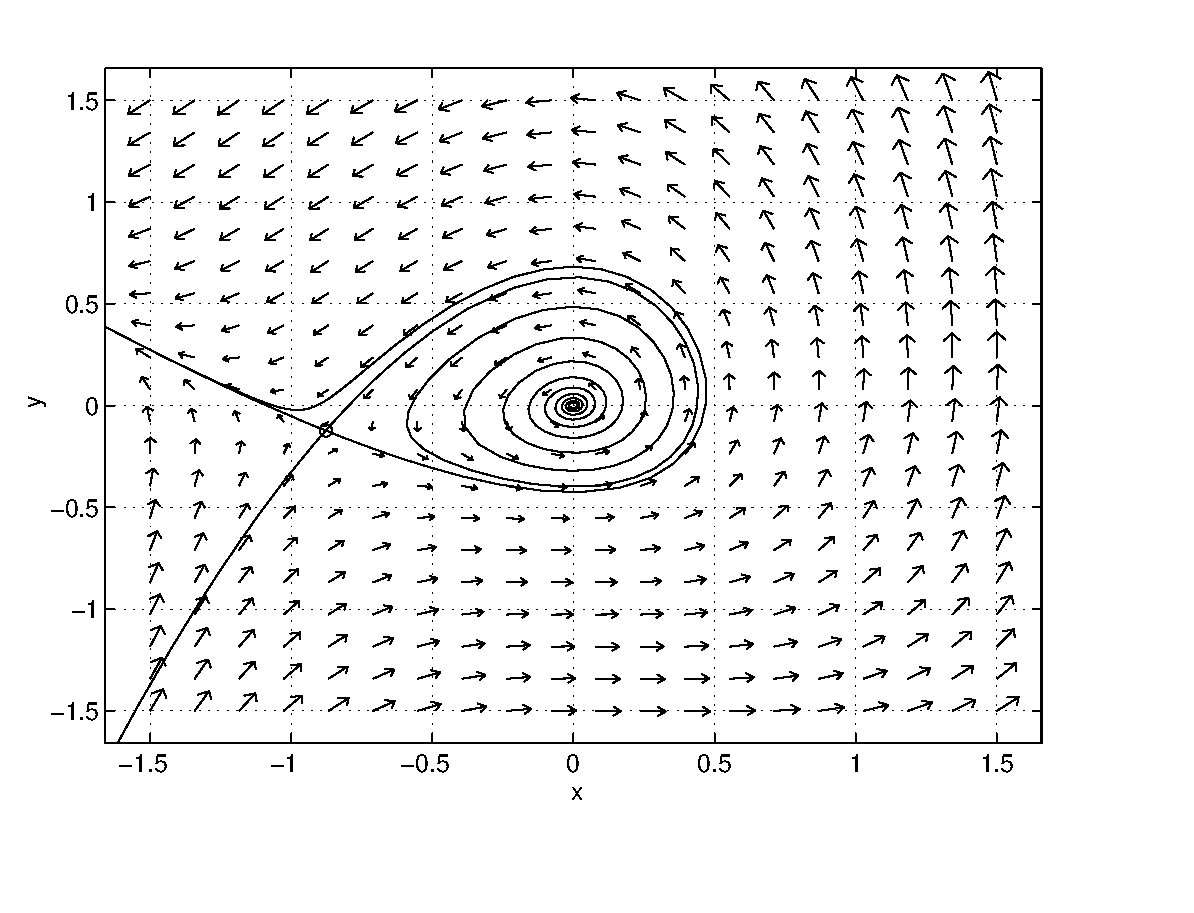
\psfig{file=figures/homobif3.eps,height=2.0in}}
		\vspace*{-0.2in}		
	$\rho=-0.07$ \hspace{1.8in} $\rho=0.07$ 
		\hspace{1.8in} $\rho=0.14$
	  \caption{Phase planes for the differential equation 
	\protect\Ref{E:homobif}. }
           \label{F:homobif}
\end{figure}

Use {\sf pplane5} to plot the phase plane portraits of \Ref{E:homobif}
for $\rho=-0.07$, $\rho=0.07$, and $\rho=0.14$.  (These phase portraits 
are most easily drawn by having {\sf pplane5} find the saddle point and
then plot the stable and unstable orbits.)  The phase portraits are 
displayed in Figure~\ref{F:homobif}.  

From the numerical calculations we see that a standard Hopf bifurcation 
to a stable limit cycle occurs as $\rho$ 
increases through $0$ --- but that limit cycle disappears by the
time $\rho=0.14$.   We discuss homoclinic bifurcations in more detail 
in Section~\ref{S:bifurcation}.  For the moment, just note that such 
transitions are possible.  In bifurcation diagrams, a homoclinic 
bifurcation  is indicated by having a branch of periodic solutions
terminate with a black dot.  In Figure~\ref{F:homobifdiag} we show the 
bifurcation diagram for the system of differential equations 
\Ref{E:homobif} for $\rho$ between $-0.1$ and $0.15$.  Note that there
are branches for two equilibria and a 
branch of limit cycles\index{branch of limit cycles} 
beginning at a Hopf bifurcation and ending at a homoclinic bifurcation.
In this particular bifurcation diagram we have labeled all pieces
of information including the equilibria and their types, the 
bifurcations and their types, and the limit cycles.


\begin{figure}[htb]
           \centerline{%
           \psfig{file=figures/homobifdiag.eps,height=2.5in}}
  \caption{Schematic bifurcation diagram for the differential equation
    \protect\Ref{E:homobif} indicating a branch of stable limit cycles
        ending in a homoclinic bifurcation.}
           \label{F:homobifdiag}
\end{figure}
\index{diagram!bifurcation}

Homoclinic bifurcations are global bifurcations; the change in the phase 
portrait does not occur in a small neighborhood of an equilibrium.  For 
this reason we cannot detect homoclinic bifurcations analytically as we 
did for saddle-node bifurcations in \Ref{E:DCSN} and \Ref{E:DCSN2} and Hopf bifurcations in \Ref{E:NCHB}.




\subsection*{Reading Bifurcation Diagrams}

Planar systems of differential equations that model applications often
lead to complicated bifurcation diagrams.  We will see an example
of this complexity in Section~\ref{S:CSTR} when we study a model for a 
continuous flow stirred tank chemical reactor.  
Now we discuss the information contained in the hypothetical bifurcation 
pictured in Figure~\ref{F:hypo}. In words we describe the six bifurcations
contained in this hypothetical bifurcation diagram. 

\begin{figure}[htb]
           \centerline{%
           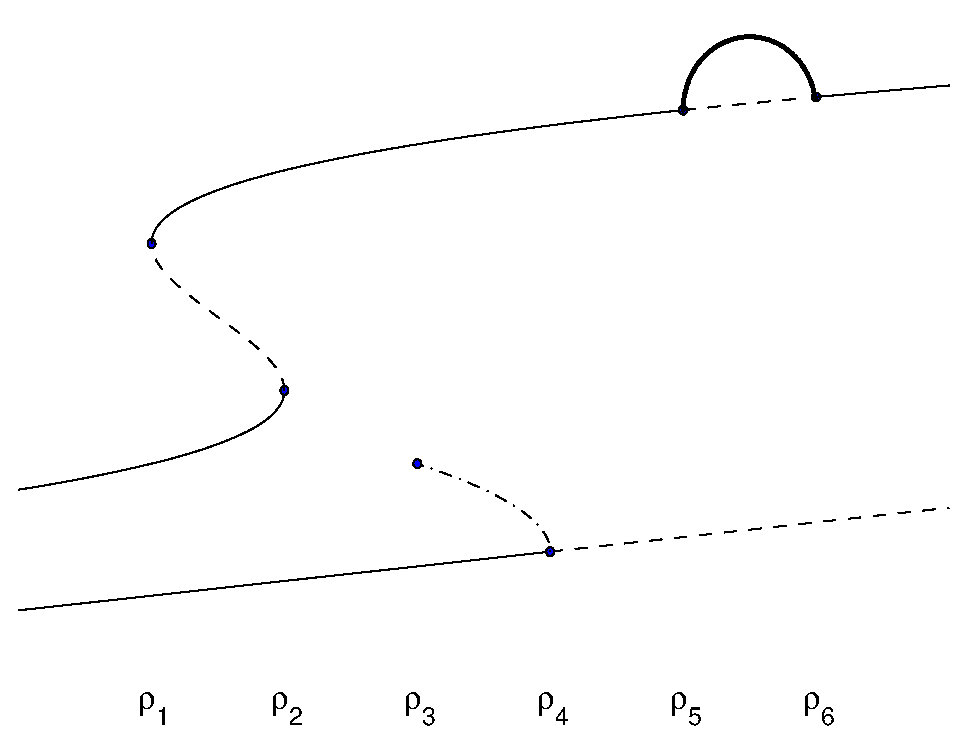
\psfig{file=figures/hypo.eps,height=3.0in}}
  	   \caption{A hypothetical schematic bifurcation diagram for a planar 
	  system of differential equations with six bifurcation points.} 
           \label{F:hypo}
\end{figure}
\index{diagram!bifurcation}

For $\rho<\rho_1$
there are two stable equilibria.  There is a saddle-node bifurcation 
at $\rho_1$ where two additional equilibria --- one stable and one 
unstable --- are created.  At $\rho_2$ there is a second saddle-node 
bifurcation where two of the four equilibria disappear.  
\index{bifurcation!saddle-node}

As $\rho$ increases past $\rho_3$ a homoclinic 
bifurcation\index{bifurcation!homoclinic} produces an
unstable limit cycle that disappears at a 
Hopf bifurcation\index{bifurcation!Hopf} at $\rho_4$.  
Note that the equilibrium becomes unstable at $\rho_4$.
Hopf bifurcations also occur at $\rho_5$ and $\rho_6$.   A stable
limit cycle is created at $\rho_5$ and disappears at $\rho_6$.
\index{bifurcation!Hopf}

As you can see, a  bifurcation diagram is a shorthand method for recording
an exceptional amount of information.  In subsequent sections we develop 
some of theory needed to understand the changes that are to be expected 
at each bifurcation.  

\EXER

\TEXER

\begin{exercise} \label{c9.7.1}
Show that the differential equation 
\[
\dot{x} = \rho + x^2
\]
undergoes a saddle-node bifurcation at $\rho=0$ where two equilibria 
disappear as $\rho$ increases through $0$.  Draw the bifurcation diagram 
for this differential equation.
\end{exercise}

\begin{exercise} \label{c9.7.2}
Show that the differential equation
\[
\dot{x} = \rho - x^2 + 2x
\]
undergoes a saddle-node bifurcation at $\rho=-1$ where two equilibria
appear as $\rho$ increases through $-1$.  Draw the bifurcation diagram
for this differential equation.
\end{exercise}

\begin{exercise} \label{c9.7.3}
Sketch the bifurcation diagram of the one parameter family of differential 
equations
\begin{equation} \label{E:ex2}
\dot{x} = 3x^4 - 8x^3 - 6x^2 + 24x - \rho.
\end{equation}
What is the maximum number of equilibria for \Ref{E:ex2} and for which 
values of $\rho$ does this maximum number occur? {\bf Hint:} Graph the 
function $\rho=3x^4 - 8x^3 - 6x^2 + 24x$ by finding its maxima and minima. 
\end{exercise}

\begin{exercise} \label{c9.4.1}
The unforced Van der Pol equation is: \index{Van der Pol equation}
\begin{equation*}
\begin{array}{rcl}
\dot{x} & = & \rho x - y -x^3 \\
\dot{y} & = & x.
\end{array}
\end{equation*}
Verify analytically that the origin is the only equilibrium of this equation
and that the only value of $\rho$ where that equilibrium could be a point of
Hopf bifurcation is $\rho=0$.  Use {\sf pplane5} to verify that there is a 
unique limit cycle when $\rho>0$.
\end{exercise} 


\begin{exercise} \label{c9.4.2}
At what point $(x_0,y_0)$ is it possible for the differential equation 
\begin{equation*}  \label{E:hopfex}
\begin{array}{rcl}
\dot{x} & = & -4 +3x -4y +x^2 -2y^2 \\
\dot{y} & = & -21 -(1+\rho)y + 7x^2 - 3xy
\end{array}
\end{equation*}
to have a Hopf bifurcation when $\rho=0$.  
\end{exercise}



\CEXER

\begin{exercise} \label{e:source}
Change the sign of the $\dot{y}$ equation in \Ref{E:ssys}, obtaining the 
system of differential equations:  
\[
\begin{array}{rcl}
\dot{x} & = & x^2 - \rho + y \\
\dot{y} & = & y(x^2+1).  \end{array}
\]
Show that a saddle-node bifurcation occurs at $\rho=0$ in this system by 
plotting phase portraits for $\rho=-1$ and $\rho=1$.  How do the 
phase portraits of this system differ from those of \Ref{E:ssys} 
given in Figure~\ref{F:ssys}.
\end{exercise}

\begin{exercise}  \label{e:uHopf}
Change the sign of the $y^3$ term in the $\dot{y}$ equation in 
\Ref{E:Hopfbif} and obtain the system of differential equations:
\[
\begin{array}{rcl}
\dot{x} & = & y \\
\dot{y} & = & -x + \rho y + y^3.  \end{array}
\]
Use {\sf pplane5}\index{\computer!pplane5}
to plot the phase portraits of this system when 
$\rho=-1$ and $\rho=1$.  Describe the differences between these phase portraits
and those in Figure~\ref{F:Hopfbif}. Draw the bifurcation diagram.
\end{exercise}

\begin{exercise} \label{c9.7.4}
Consider the system of differential equations
\begin{equation*}  \label{E:hbifex}
\begin{array}{rcl}
\dot{x} & = & -1 + \rho + 5x + 2.5y + x^2 - x^3 \\
\dot{y} & = & -5 - x + 4y - y^2.  \end{array}
\end{equation*}
\begin{itemize}
\item[(a)]  Verify that \Ref{E:hbifex} has an equilibrium at $X_0=(-1,2)$ 
when $\rho=-1$.
\item[(b)]  Show that the linearization of \Ref{E:hbifex} at $X_0$ is a 
center when $\rho=-1$.  
\item[(c)]  Let $\rho$ be a number close to $-1$.  Use {\sf pplane5} to 
determine whether \Ref{E:hbifex} has a spiral sink when $\rho<-1$ or when 
$\rho>-1$.  
\item[(d)]  Determine whether limit cycles exist for $\rho<-1$ or for 
$\rho>-1$.
\item[(e)]  Find an approximate value of $\rho$ at which \Ref{E:hbifex}
has a second Hopf bifurcation.
\end{itemize} 
\end{exercise}

\begin{exercise} \label{c9.7.5}
Consider the differential equation:
\begin{equation*} \label{e:homo}
\begin{array}{rcl}
\dot{x} & = &  y \\
\dot{y} & = &  -\rho + y + x^2 + xy
\end{array}
\end{equation*}
\begin{itemize}
\item[(a)]  Show analytically that \Ref{e:homo} has two equilibria at 
$(\pm\sqrt{\rho},0)$ when $\rho>0$. 
\item[(b)]  Show analytically that the equilibrium at $(\sqrt{\rho},0)$ is 
always a saddle, while the equilibrium at $(-\sqrt{\rho},0)$ is a spiral sink 
when $1<\rho<97$.  
\item[(c)]  Use {\sf pplane5} to show that the phase portrait of \Ref{e:homo} 
has a homoclinic trajectory between $\rho=1.7$ and $\rho=1.8$.  
\end{itemize}
\end{exercise}

\noindent In Exercises~\ref{c9.4.3a} -- \ref{c9.4.3c}, 
consider the system of differential equations \Ref{E:duff}
\begin{equation*}  \label{E:duff}
\begin{array}{rcl}
\dot{x} & = & y - \mu x - x^2   \\
\dot{y} & = & -x - \mu y + x^2.
\end{array}
\end{equation*}
\begin{exercise} \label{c9.4.3a}
Show that \Ref{E:duff} undergoes a Hopf bifurcation near the origin when 
$\mu=0$.  Sketch the qualitative phase portraits on either 
side of the Hopf bifurcation.
\end{exercise}
\begin{exercise} \label{c9.4.3b}
Show that another bifurcation takes place in \Ref{E:duff} near 
$\mu\approx -0.1$.  Sketch the new phase portrait that appears near this 
bifurcation.    
\end{exercise}
\begin{exercise} \label{c9.4.3c}
For each of the three different phase portraits examined in 
Exercises~\ref{c9.4.3a} and \ref{c9.4.3b} identify the region of initial 
conditions in the square $-4\leq x,y \leq 4$ where solutions stay within the 
square in forward time and the region where solutions stay within the square 
in both forward and backward time.
\end{exercise}

\begin{exercise} \label{c9.4.4}
Use {\sf pplane5} to determine whether there are small amplitude periodic 
solutions to \Ref{E:hopfex} at $\rho>0$ or at $\rho<0$.
\end{exercise}



\section{The Continuous Flow Stirred Tank Reactor} 
\label{S:CSTR} \index{CSTR}

Perhaps the simplest chemical engineering model of a chemical
reaction is the CSTR --- the continuous flow stirred tank
chemical reactor.  In the CSTR we imagine that a reactant flows
into a vessel and undergoes a single heat producing reaction to
form inert products.  The concentration of the reactant inside
the vessel is denoted by $c$ and the temperature of the fluid
inside the vessel is denoted by $T$.  The assumption that the
tank is well stirred is interpreted mathematically to mean that
$c$ and $T$ are constant everywhere in the vessel.  The CSTR
model describes how $c$ and $T$ evolve in time. 

The CSTR is pictured schematically in Figure~\ref{F:CSTRs}.  We assume 
that the reactant flows into a unit volume vessel at a constant rate 
$r$ and that the product flows out of the vessel at the same rate.  
The fluid that flows into the vessel is called the {\em feed\/}.  
We assume that the temperature of the feed is held constant at
$T_f$ and that the reactant concentration of the feed is $c_f$.
We also assume that the vessel is surrounded by a coolant whose
temperature $T_c$ is held constant.  

\begin{figure}[htb]
           \centerline{%
	   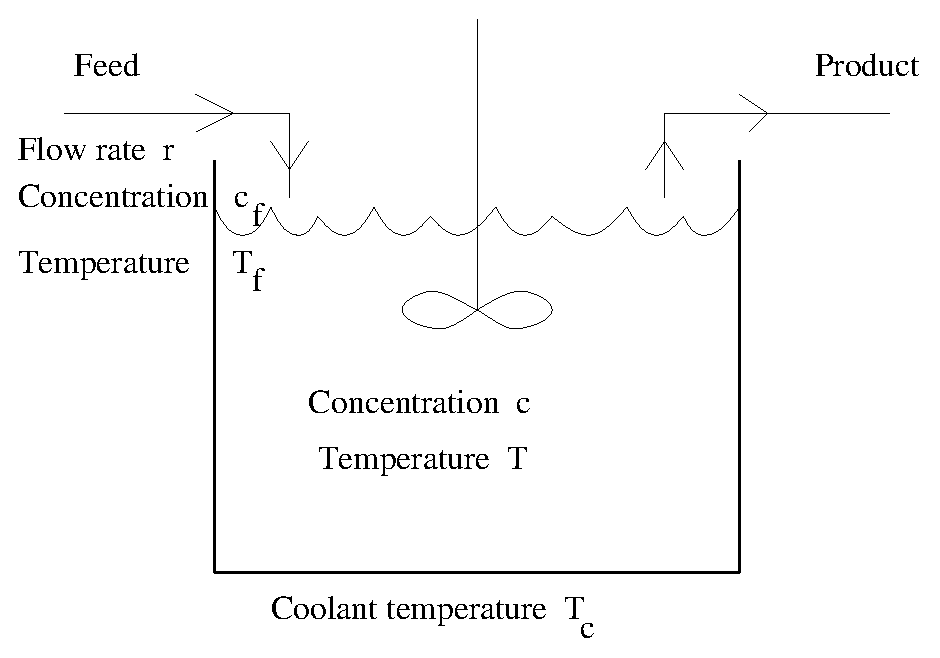
\psfig{file=figures/CSTR.eps,height=3.0in}}
           \caption{Schematic diagram for CSTR.}
           \label{F:CSTRs}
\end{figure}\index{CSTR}


\subsection*{The Reactionless CSTR}
\index{CSTR}

Ignoring the effects of the chemical reaction, the model
equations describing the time evolution of the temperature and
concentration of the reactant in the vessel are:
\arraystart
\begin{equation} \label{e:CSTRlin}
\begin{array}{rcl}
\dps\frac{dc}{dt} & = & r(c_f-c) \\
\dps\frac{dT}{dt} & = & r(T_f-T) + k(T_c-T),
\end{array}
\end{equation}
\arrayfinish   \index{CSTR} 
where $k$ is a lumped parameter that depends on a variety of
physical quantities including heat transfer area and specific
heat.  

So far, the model in \Ref{e:CSTRlin} is an inhomogeneous uncoupled system
of linear differential equations.  We have assumed that the concentration 
of the reactant grows exponentially to the feed concentration at rate
$r$.  The fate of the temperature inside the vessel is less
clear, as we have assumed that the temperature grows exponentially to 
the feed temperature at rate $r$ and simultaneously grows
exponentially to the coolant temperature at rate $k$ (that is
just Newton's law of cooling\index{Newton's law of cooling}).  
At this point, we have not modeled the effects of the chemical reaction 
on concentration and temperature inside the vessel --- though we have modeled 
how the external variables such as feed temperature and concentration and 
the coolant temperature affect the concentration and temperature inside the 
vessel.  For this reason, this model is called the {\em reactionless\/} CSTR. 
Before continuing with the modeling, we 
nondimensionalize\index{nondimensionalize} the variables, as 
engineers prefer to do.

In this model, we have assumed implicitly that concentration and
temperature are positive quantities.  For concentration this is
clearly a reasonable assumption.  For temperature this means
that we are measuring temperature from absolute zero.  Suppose
that we let  \index{scaling}
\[
x(t) = \frac{c(\frac{t}{k})-c_f}{c_f} \AND 
y(t) = \frac{T(\frac{t}{k})-T_f}{T_f}
\]
be scaled concentration and temperature.  We have normalized $x$
and $y$ to measure deviation from the feed concentration and
temperature, and we have scaled $c$ and $T$ by $c_f$ and $T_f$
so that the state variables $x$ and $y$ are nondimensional ---
they have no physical units attached to them.  In addition, we
have scaled time by the lumped rate constant $k$.  (Chemical engineers
do not usually scale time in the equations, since $k$ is a 
parameter that can be controlled in experiments.) Next, let 
\[
\eta = \frac{T_c-T_f}{T_f} \AND \rho = \frac{r}{k}
\]
be the nondimensionalized coolant temperature and flow rate,
respectively.  Note that the fact that all physical quantities
were assumed to be positive leads to the restrictions
\[
x, y,\eta >-1  \AND \rho>0.
\]

Observe that 
\[
\frac{dx}{dt}(t)=\frac{1}{kc_f}\frac{dc}{dt}\left(\frac{t}{k}\right) \AND
\frac{dy}{dt}(t)=\frac{1}{kT_f}\frac{dT}{dt}\left(\frac{t}{k}\right).
\]
Coupling this observation with \Ref{e:CSTRlin} yields the equations 
for the reactionless CSTR in nondimensionalized form:
\begin{eqnarray}
\dot{x} & = & -\rho x \label{e:ndCSTRlina} \\
\dot{y} & = & -(\rho+1)y + \eta. \label{e:ndCSTRlinb}
\end{eqnarray}\index{CSTR}
The solution to \Ref{e:ndCSTRlina} is 
\[
x(t) = e^{-\rho t}x_0,
\]
and, in the absence of a reaction, the scaled concentration
decays exponentially to $x=0$, that is, to the feed
concentration.

The solution to \Ref{e:ndCSTRlinb} is slightly more complicated
to obtain in closed form, as this is an example of an
inhomogeneous linear equation.  Using 
superposition\index{superposition}, we can find
the general solution to the inhomogeneous equation by finding
one solution to the inhomogeneous\index{inhomogeneous} 
equation and adding in all
solutions to the homogeneous\index{homogeneous} equation.  
In this case, it is easy to find a constant solution to the 
inhomogeneous equation.  Just set
\begin{equation}  \label{e:basetemp}
y = \frac{\eta}{\rho+1},
\end{equation}
and check that this constant is a solution to
\Ref{e:ndCSTRlinb}.  As we know,
\[
y(t) = e^{-(\rho+1)t}K
\]
is the general solution to the homogeneous equation, and
\[
y(t) = e^{-(\rho+1)t}K + \frac{\eta}{\rho+1}
\]
is the general solution to \Ref{e:ndCSTRlinb}.  Thus,
temperature decays exponentially to \Ref{e:basetemp}, the
coolant temperature in nondimensionalized form scaled by the
nondimensionalized flow rate\index{flow rate}.

\subsection*{The CSTR}
\index{CSTR}
 
Next we consider the effects of the reaction.  For thermodynamic
reasons, which we do not discuss here, we assume that the
reaction depletes the reactant at a temperature dependent rate
proportional to concentration times the {\em Arrhenius\/} term
\index{Arrhenius term} $A(y)$ where
\[
A(y) = \exp\left(\frac{\gamma y}{y+1}\right)
\]
and $\gamma$ is the {\em activation 
energy\/}\index{activation energy}.  Since the
reaction is heat producing, we also assume that the temperature
of the reactant increases at a rate proportional to $cA(y)$.
Since the concentration $c$ is proportional to $x+1$, these
assumptions lead to the nonlinear system of differential
equations
\begin{equation*} \label{e:CSTR}
\begin{array}{rcl}
\dot{x} & = & -\rho x  - Z(x+1)A(y) \\
\dot{y} & = & -(\rho+1)y + \eta + hZ(x+1)A(y),
\end{array}
\end{equation*}
where $Z$ and $h$ are proportionality constants.  In this form
the equations have two state variables $x,y$ and five constants
$\rho,\eta,\gamma,Z,h$.  (The CSTR equation in {\tt e12\_3\_5.pps} has
$\gamma=4$ so that there are just four parameters.)

\subsection*{Numerical Solution of the CSTR}
\index{CSTR}

It is a difficult problem to determine the phase portraits for
the CSTR equations for all values of the five constants. Here we
use {\sf pplane5} to indicate some of the different phase
portraits that can occur in these equations.  In order to
simplify the task, we fix values for all parameters except
the nondimensionalized flow rate $\rho$.  We set
\begin{equation}   \label{e:CSTRparam}
\gamma=4, \quad \eta=-0.75, \quad Z=0.5, \quad h =3.
\end{equation}
Numerical experimentation on the rectangle $-0.75\leq x
\leq 0.5$, $-0.75\leq y\leq 0.75$ shows the following.  There are 
three possible equilibria --- one at high temperature ($y\sim 0.1$), 
one at medium temperature ($y\sim -0.1$), and one at low
temperature ($y\sim -0.5$).  For these parameter values, the 
equilibrium at medium temperature is always a saddle and the 
equilibrium at low temperature is always a 
sink\index{sink}.  We present the 
phase portraits for five values of the nondimensionalized 
flow rate\index{flow rate}
$\rho$.  The results are as follows:  
\begin{itemize}
\item[$\rho=0.495$] The only equilibrium is the low temperature 
equilibrium and it is a nodal sink. 
\item[$\rho=0.520$] There are three equilibria. The high 
temperature spiral source and the medium temperature saddle appear
as $\rho$ is increased.  Note that the stable orbit of the 
saddle connects directly to the spiral source.
\item[$\rho=0.545$] The high temperature equilibrium is a spiral 
sink and the stable orbit of the saddle connects to a limit 
cycle.  At this parameter value, there are two stable equilibria.
\index{limit cycle} \index{stable!orbit}
\item[$\rho=0.570$] There are still three equilibria, but the 
time-periodic solution has disappeared.  The unstable orbit of 
the saddle now connects to the high temperature spiral sink. The
low temperature sink is a spiral sink and there are two stable
spiral sinks. 
\item[$\rho=0.720$] The only remaining equilibrium is the high
temperature spiral sink.  The saddle and the low temperature 
sink have coalesced and disappeared.  (Presumably the low temperature 
spiral sink became a nodal sink before it coalesced with the saddle.)
\end{itemize}

These calculations show that the phase portrait of the CSTR changes 
between successive values of $\rho$, that is, we have shown that 
there are at least four bifurcation values in the CSTR as $\rho$ 
is varied.  The five different phase planes are shown in Figure~\ref{F:CSTR}.


\begin{figure}
           \centerline{%
	   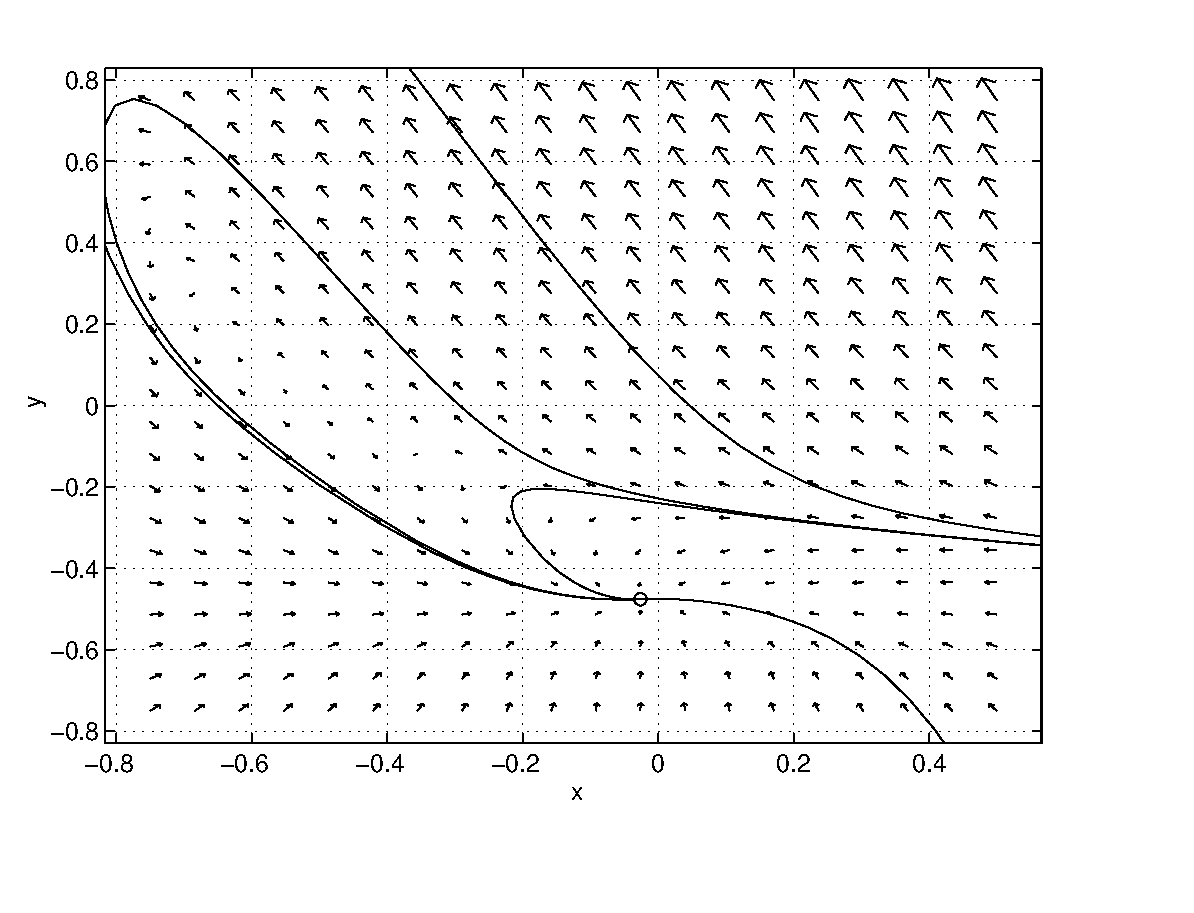
\psfig{file=figures/cstr495.eps,height=2.1in}
	   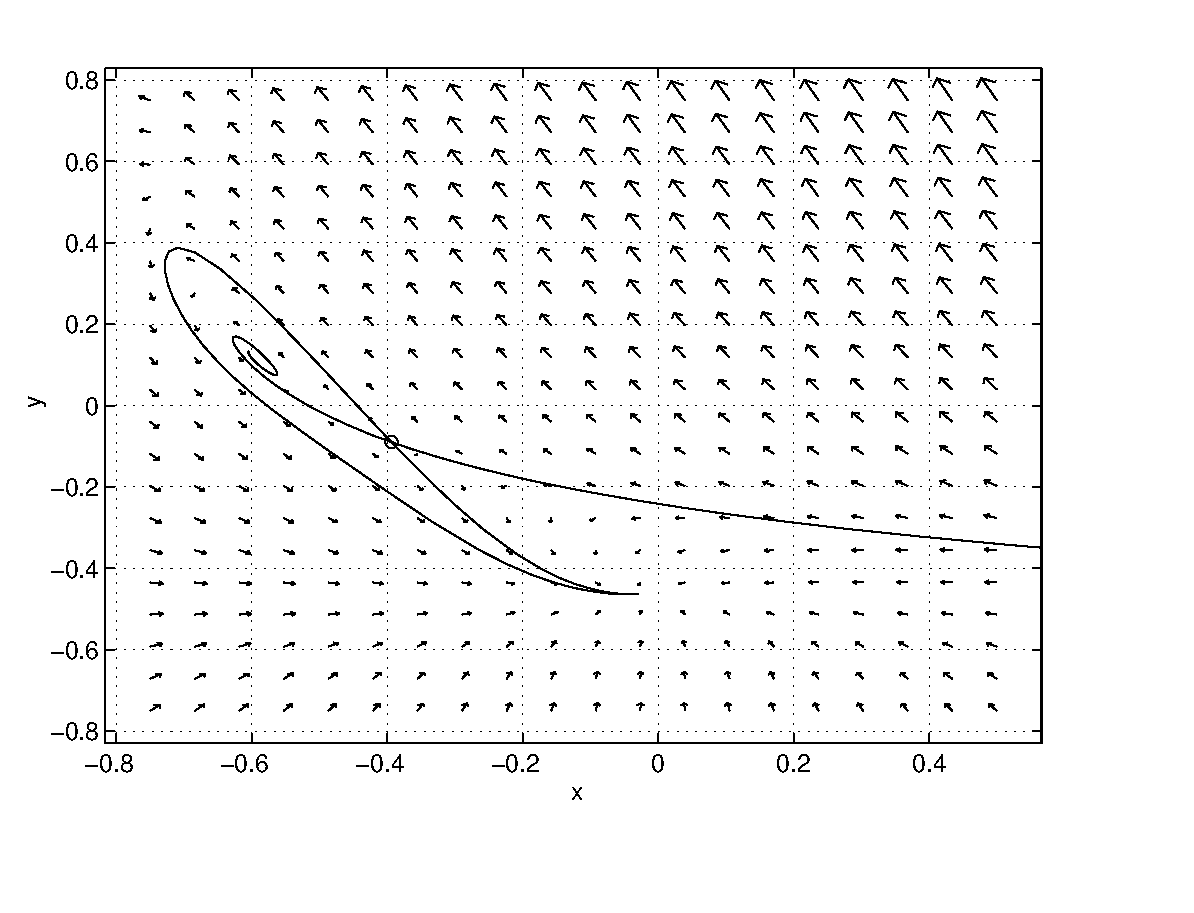
\psfig{file=figures/cstr52.eps,height=2.1in}}	
		\vspace*{-0.2in}	
		$\hspace{1.2in} \mbox{$\rho=0.495$ \hspace{2.0in} $\rho=0.52$}$
           \centerline{%
	   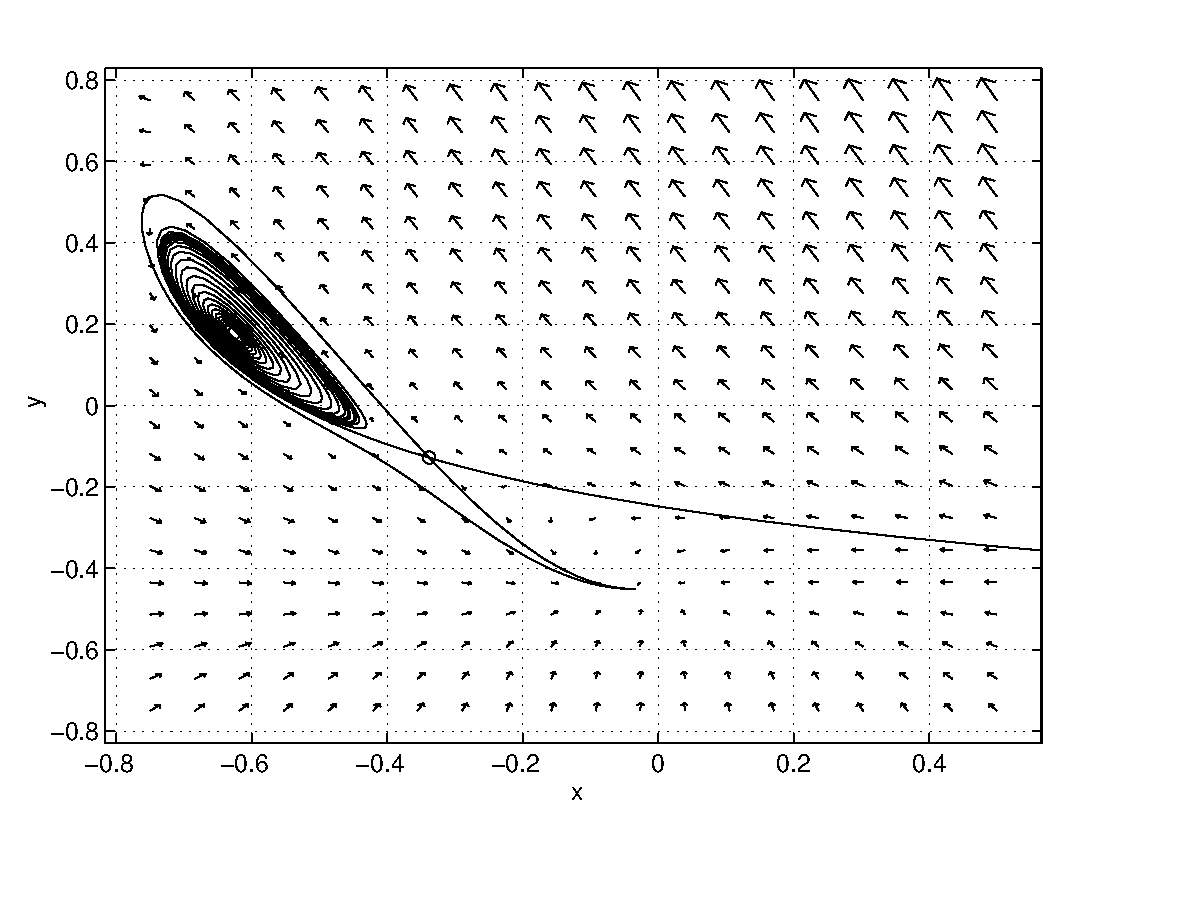
\psfig{file=figures/cstr545.eps,height=2.1in}
	   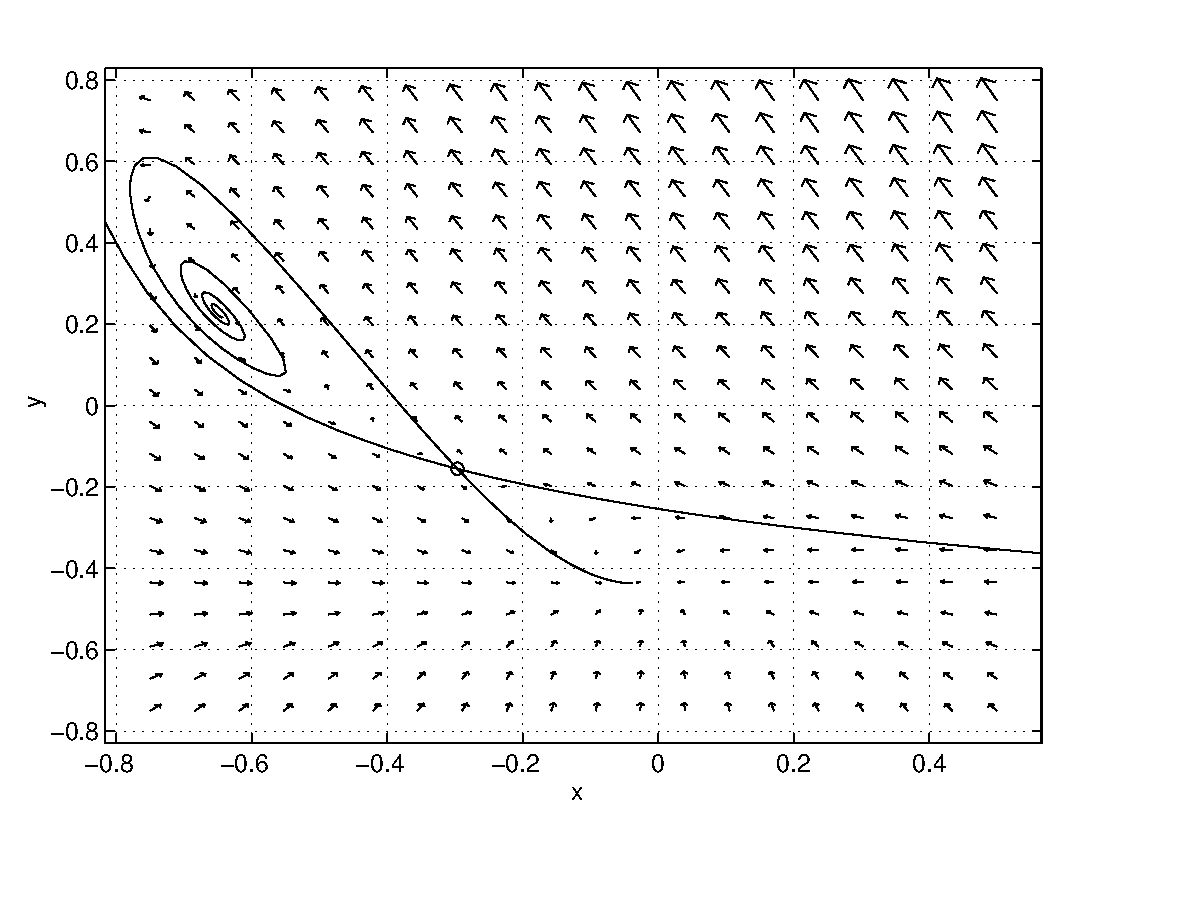
\psfig{file=figures/cstr57.eps,height=2.1in}}
		\vspace*{-0.4in}
		
		$\hspace{1.2in} \mbox{$\rho=0.545$ \hspace{2.0in} $\rho=0.57$}$
		\vspace{0.4in}
	   \centerline{%
           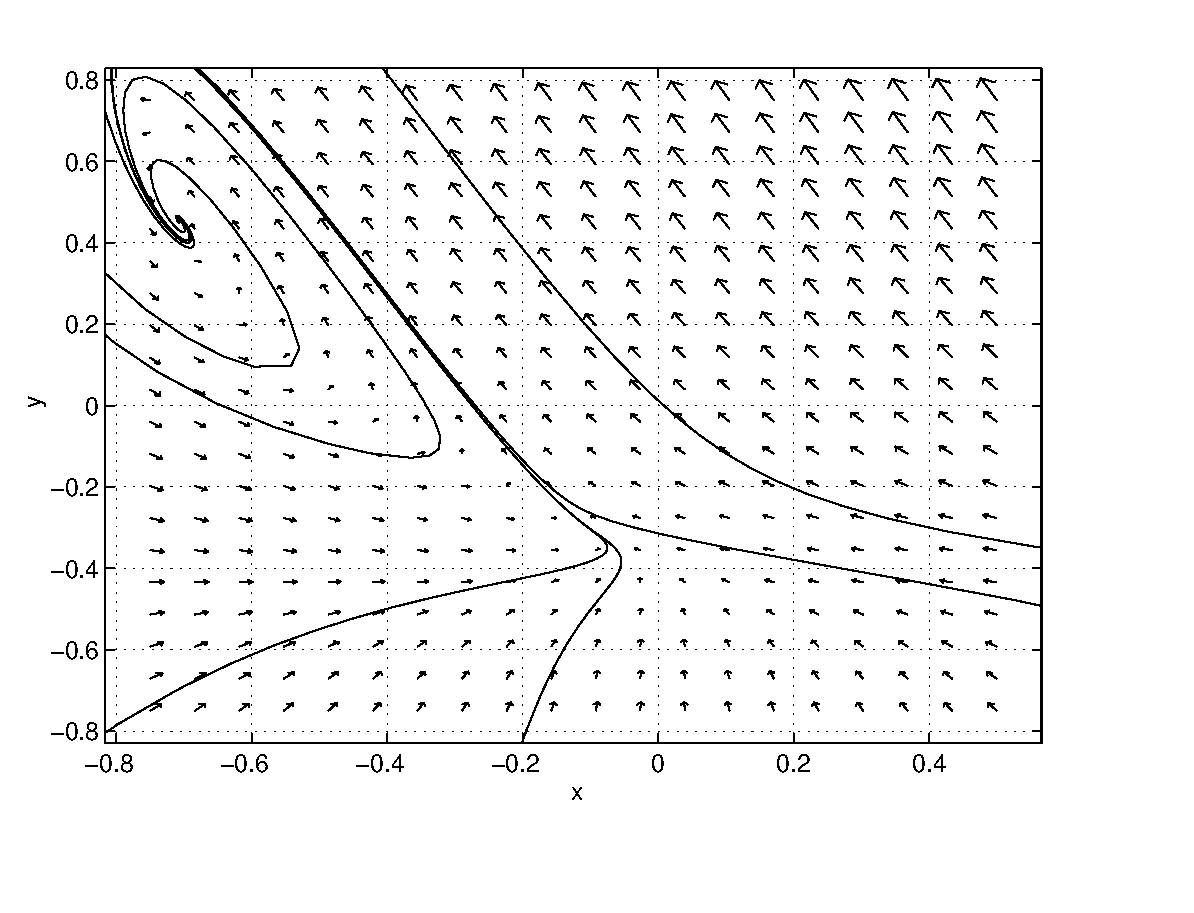
\psfig{file=figures/cstr72.eps,height=2.1in}}
 		\vspace*{-0.8in}
		
		\hspace{2.6in} $\rho=0.72$
          \caption{Phase portraits of CSTR \protect\Ref{e:CSTR} 
	with $\gamma=4$, $\eta=-0.75$, $Z=0.5$, $h =3$.}
           \label{F:CSTR}
\end{figure}


\subsection*{Bifurcations in the CSTR}
\index{CSTR}


The observed bifurcations in the CSTR divide into local and global 
bifurcations, as we now discuss.

As we saw in Section~\ref{S:bifurcation}, local bifurcations are of two 
types: steady-state (saddle-node) and Hopf. \index{bifurcation!steady-state} 
\index{bifurcation!Hopf}  For example, in Figure~\ref{F:CSTR}, we see that as 
the parameter $\rho$ is decreased from $0.52$ to $0.495$ the middle and high 
temperature equilibria collide and disappear at a saddle-node bifurcation.  
See Exercise~\ref{E:CSTR5} for further verification of this fact.  Similarly,
between the values of $\rho=0.57$ and $\rho=0.72$ the low and middle 
temperature equilibria collide and disappear.  We presume that a  
saddle-node bifurcation has also occurred in this parameter regime.

A different bifurcation occurs as $\rho$ increases from
$0.52$ and $0.545$.  In this range, the high temperature spiral
changes from a source to a sink.  For this change to occur,
there must be a parameter value where the high temperature
equilibrium is a center.  Since a time periodic solution
is found in the phase portrait of the CSTR at $\rho=0.545$, we 
conclude that a Hopf bifurcation has occurred in this parameter region.

Both of these local bifurcations occur at parameter values where
there is a nonhyperbolic equilibrium. As we noted, Hopf
bifurcation occurs at a parameter value where a center is
present, while steady-state bifurcation occurs at a parameter value where 
an equilibrium has a Jacobian matrix with a zero eigenvalue --- typically 
a saddle-node.  

A global bifurcation\index{bifurcation!global}, one in which the bifurcation
in phase portraits occurs away from equilibria, is present in the CSTR 
between $\rho=0.545$ and $\rho=0.57$.  In this region, the periodic solution 
grows until it touches the saddle point.  At that point, one branch of 
the stable orbit and one branch of the unstable orbit of the 
saddle are identical.  Thus, there is a trajectory that limits
on the saddle point in both forward and backward time.  As we 
saw in Section~\ref{S:bifurcation} such trajectories are called 
{\em homoclinic\/} trajectories and such bifurcations are called 
{\em homoclinic bifurcations\/}.  \index{trajectory!homoclinic} 
\index{bifurcation!homoclinic}  Note the similarity between the phase 
portraits in Figure~\ref{F:homobif} and the middle phase portraits in 
Figure~\ref{F:CSTR}.

There are other global bifurcations that we have not seen in 
these equations.  Two periodic solutions can collide and both 
disappear (just like the saddle-node steady-state bifurcation 
where two equilibria collide and disappear).  This bifurcation is
discussed in Section~\ref{S:GlobalBif}.  Another global 
bifurcation occurs when the stable orbit of one saddle point 
coincides with the unstable orbit of another saddle point.  
This bifurcation is called a {\em saddle-saddle\/} connection.  
The homoclinic bifurcation is a special case of a saddle-saddle 
connection where the two saddle points are the same.
\index{saddle-saddle connection}  See Section~\ref{S:bifurcation}.

\subsection*{Bifurcation Diagrams}
\index{diagram!bifurcation}

The discussion of transitions in the 
CSTR\index{CSTR} can be summarized by the use of a 
{\em bifurcation diagram\/}, as introduced in Section~\ref{S:bifurcation}.  
In a bifurcation diagram we graph the equilibria {\em and\/} periodic 
solutions of equations as a function of the parameter $\rho$.  In 
bifurcation diagrams: \index{diagram!bifurcation}
\begin{itemize}
\item	A saddle-node bifurcation appears as a turning point in 
	a branch of equilibria.
\item	A Hopf bifurcation appears as a change in stability along 
	a branch of equilibria.
\item	A homoclinic bifurcation is noted by a sudden ending of a 
	branch of periodic solutions.
\end{itemize}
In the CSTR equations we have numerical evidence for two saddle-node 
bifurcations, a Hopf bifurcation, and a homoclinic bifurcation.  
This information is illustrated in the bifurcation diagram in 
Figure~\ref{F:CSTRbif}.  Bifurcation diagrams contain an enormous amount 
of information --- and it takes practice to learn to read them.  For 
example, suppose $\rho$ is fixed to be $0.545$ in Figure~\ref{F:CSTRbif}.
Then we may surmise that there are three equilibria of the CSTR equations
at that value of $\rho$ --- the low and high temperature equilibria are 
asymptotically stable while the middle temperature one is not --- and an 
unstable limit cycle (that surrounds the high temperature equilibrium).

\begin{figure}[htb]
           \centerline{%
	   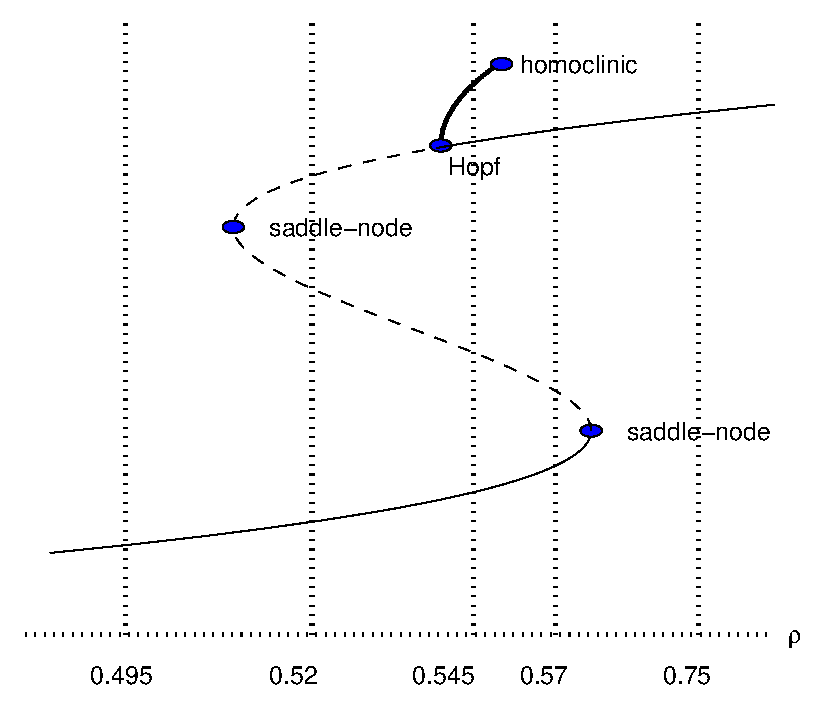
\psfig{file=figures/cstrbif.eps,width=4.0in}}
           \caption{Schematic bifurcation diagram for the CSTR}
           \label{F:CSTRbif}
\end{figure}


\EXER

\CEXER

\begin{exercise}  \label{E:CSTR5}
Consider the CSTR equations \Ref{e:CSTR} with parameters 
\Ref{e:CSTRparam}. Set $\rho=0.5$ and use 
{\sf pplane5}\index{\computer!pplane5} to verify 
that there are two equilibria --- a low temperature nodal sink 
and a middle temperature saddle-node equilibrium.  Then change 
$\rho$ to $0.505$ and verify that the saddle-node has split 
into two equilibria --- a saddle and a spiral source.
\end{exercise}

\begin{exercise} \label{c9.2.2}
Use {\sf pplane5} to explore the CSTR equations \Ref{e:CSTR} with
parameters:
\[
h=2, \quad Z=0.5, \quad \eta=-0.5, \quad \gamma=5,
\]
for various values of the parameter $\rho$ between $0.46$ and 
$0.51$.  Describe all equilibria and all periodic solutions that 
you find, and how they change as $\rho$ is varied.
\end{exercise}



\section{The Remaining Global Bifurcations} 
\label{S:GlobalBif}

We have seen one kind of global bifurcation: the homoclinic bifurcation. 
There are two other global bifurcations that are likely to occur in planar 
systems of differential equations depending on one parameter:  a saddle-node
bifurcation of periodic solutions and a heteroclinic trajectory connecting two
different saddle points.

\subsection*{Saddle-Node Bifurcations of Periodic Solutions}

Typically, planar systems have a periodic solution that is not a limit cycle 
when two limit cycles collide and disappear --- very much like the collision 
and destruction of two equilibria in a saddle-node bifurcation.  We illustrate 
this kind of collision using phase--amplitude equations and {\sf pplane5}.
Indeed, the collision of periodic solutions corresponds to a saddle-node 
bifurcation of equilibria in the amplitude equation.
\index{bifurcation!saddle-node}
\index{bifurcation!saddle-node!for periodic solutions}

Let $X=(x,y)$ and consider the system of differential equations 
\begin{equation*}  \label{e:papp}
\begin{array}{rcl}
\dot{x} = a(x^2+y^2,\rho)x - 3y \\
\dot{y} = a(x^2+y^2,\rho)y + 3x,
\end{array}
\end{equation*}
where $r^2=x^2+y^2$ and
\begin{equation}  \label{e:app}  
a(r^2,\rho) = \rho - (r^2-1)^2.
\end{equation} 
Recall from \Ref{e:amplitude},\Ref{e:phase} of Chapter~\ref{C:NPS}
that in polar coordinates $(r,\theta)$ the 
amplitude equation\index{amplitude!equation} is 
\[
\dot{r} = a(r^2,\rho)r
\]
and the phase equation\index{phase!equation} is
\[
\dot{\theta} = 3.
\]

Recall that zeros of the amplitude equation $a(r^2,\rho)=0$ correspond to 
periodic solutions of \Ref{e:papp}.  When $0<\rho<1$ there are two zeros of 
the amplitude equation \Ref{e:app} that occur at 
\[
r^2 = 1 \pm\sqrt{\rho}.
\]
When $\rho<0$ there are no zeros of the amplitude equation.  
It follows that the amplitude equations undergo a saddle-node 
bifurcation at $(r,\rho)=(1,0)$ and that two periodic solutions of 
\Ref{e:papp} collide and disappear.  This assertion can be 
checked using {\sf pplane5}\index{\computer!pplane5}.  
See Figure~\ref{F:papp}. Note that when $\rho=0$
the circle $r=1$ is the trajectory of a periodic solution but that periodic 
solution is {\em not\/} a limit cycle.  You can see this point by noting that 
trajectories starting at points with $r>1$ asymptote in forward time to the 
periodic solution and that solutions starting at points with $r<1$ move away 
from the unit circle in forward time.  

\begin{figure}[htb]
           \centerline{%
	   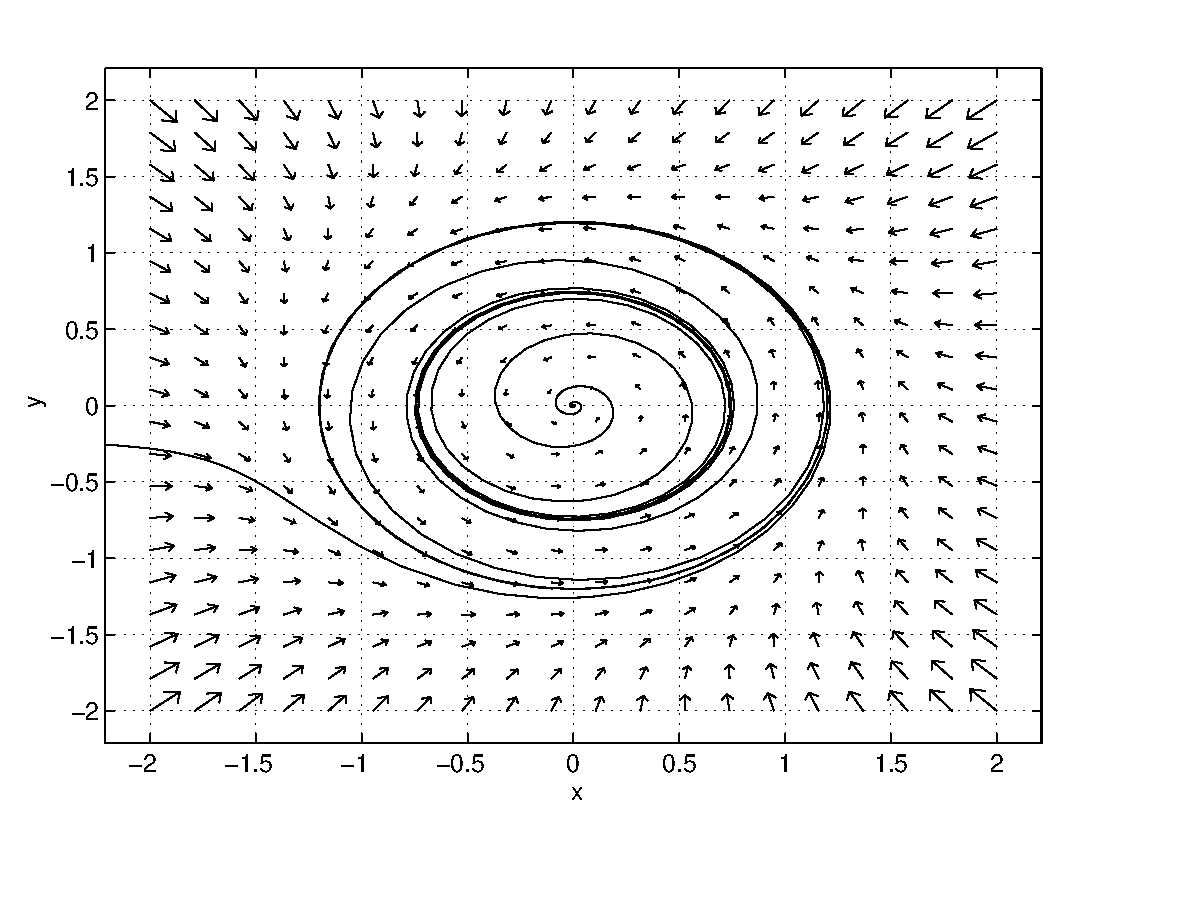
\psfig{file=figures/pappa.eps,width=2.3in}
	   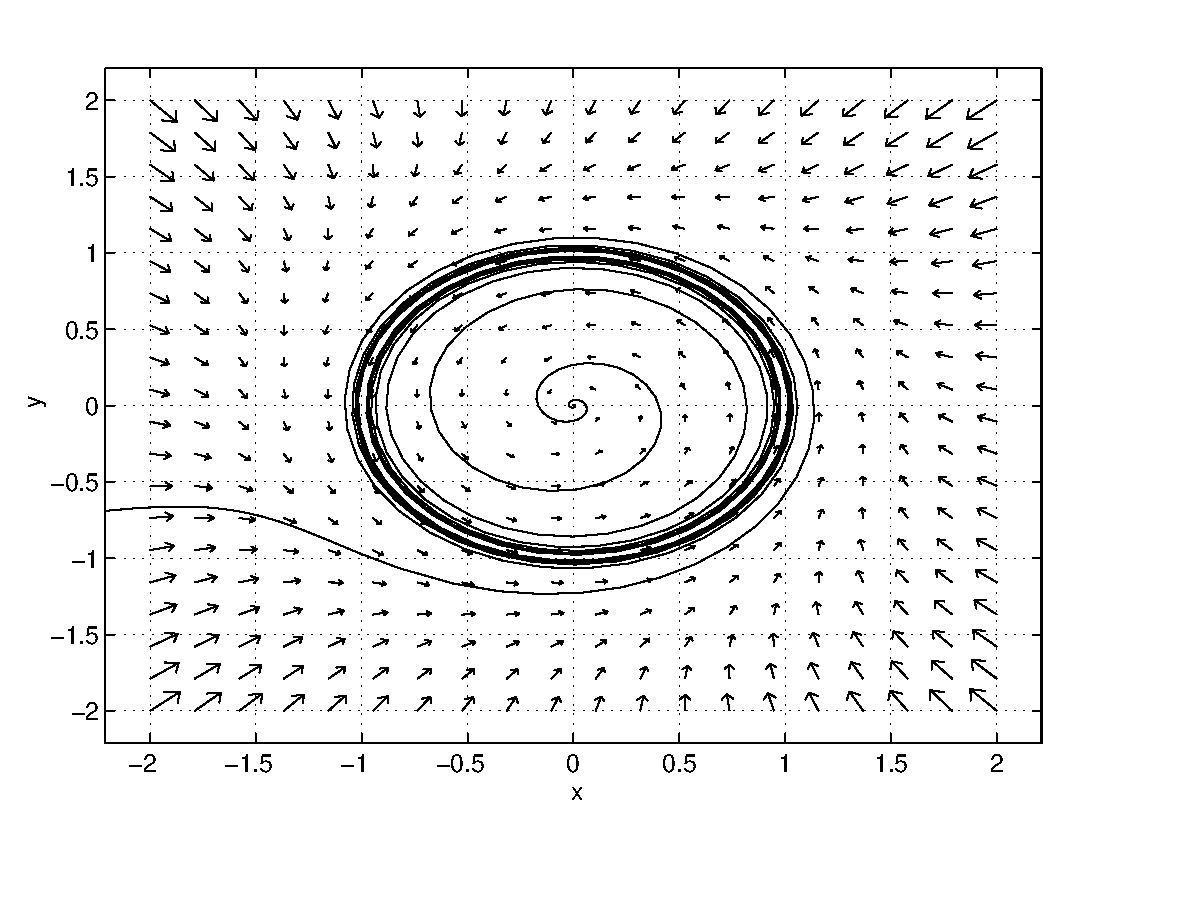
\psfig{file=figures/pappb.eps,width=2.3in}
	   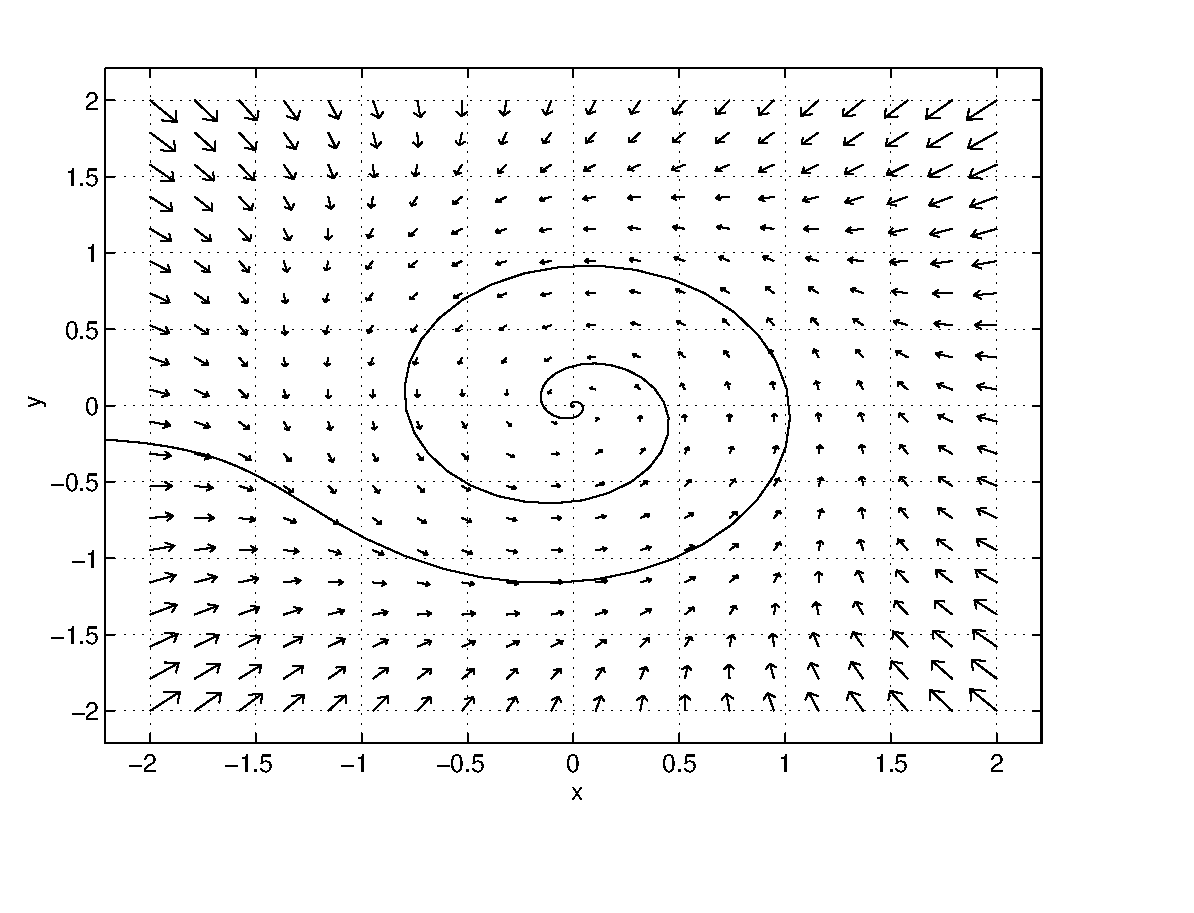
\psfig{file=figures/pappc.eps,width=2.3in}}
 	\vspace*{-0.2in}
	\hspace{0.3in} $\rho>0$  \hspace{1.9in} $\rho=0$
		\hspace{1.9in} $\rho<0$ 
           \caption{Phase portraits for \protect\Ref{e:papp}. 
Note that there are two limit cycles when $\rho>0$; one periodic solution 
when  $\rho=0$; and no periodic solutions when $\rho<0$.}
           \label{F:papp}
\end{figure}

In a sense, which we will not make precise, the annihilation of two
limit cycles in the plane through collision typically looks like the 
scenario shown in Figure~\ref{F:papp}.  



\subsection*{Saddle--Saddle Connections: Heteroclinic Trajectories}
\index{saddle-saddle connection}

In Section~\ref{S:bifurcation} we discussed the consequences of having a 
single trajectory connect a saddle point to itself.  As we have seen these 
homoclinic trajectories lead to the disappearance of a limit cycle.

When a single planar trajectory connects two different saddle points, the 
stable orbit of one saddle must become the unstable orbit of the other 
saddle.  This connecting trajectory is called a {\em heteroclinic\/} 
trajectory.\index{trajectory!heteroclinic}

We begin our discussion of heteroclinic connections with a simple example:
\begin{equation*} \label{e:hetero}
\begin{array}{rcl}
\dot{x} & = &  x^2-x  \\
\dot{y} & = &  y(0.5-x) + \rho x.
\end{array}
\end{equation*}
When $\rho=0$ the only equilibria of these equations are $(0,0)$ and 
$(1,0)$.  Note that when $y=0$ it follows that $\dot{y}=0$.  Hence
the $x$-axis is an invariant line for the dynamics of this equation. 
Moreover, a short calculation shows that both of these equilibria are 
saddle points and that the $x$-axis is the stable orbit for $(0,0)$
and the unstable orbit\index{unstable!orbit} for $(1,0)$.  
It follows that the line segment 
$(0,1)$ on the $x$-axis is a single trajectory that connects the two
equilibria.  This is an example of a heteroclinic trajectory. See
Figure~\ref{F:hetero}.  The time series for the heteroclinic trajectory 
is given in Figure~\ref{F:heteroT}.  Note the similarity to the time 
series in Figure~\ref{F:pp1dt} of the one dimensional equation 
\Ref{e:1dexample} discussed in the introduction to Chapter~\ref{C:NPS}. (In 
that example the trajectory connected $0$ in negative time to $1$ in positive
time, while in the present example the heteroclinic trajectory connects
$1$ in negative time to $0$ in positive time.)

\begin{figure}[htb]
           \centerline{%
	   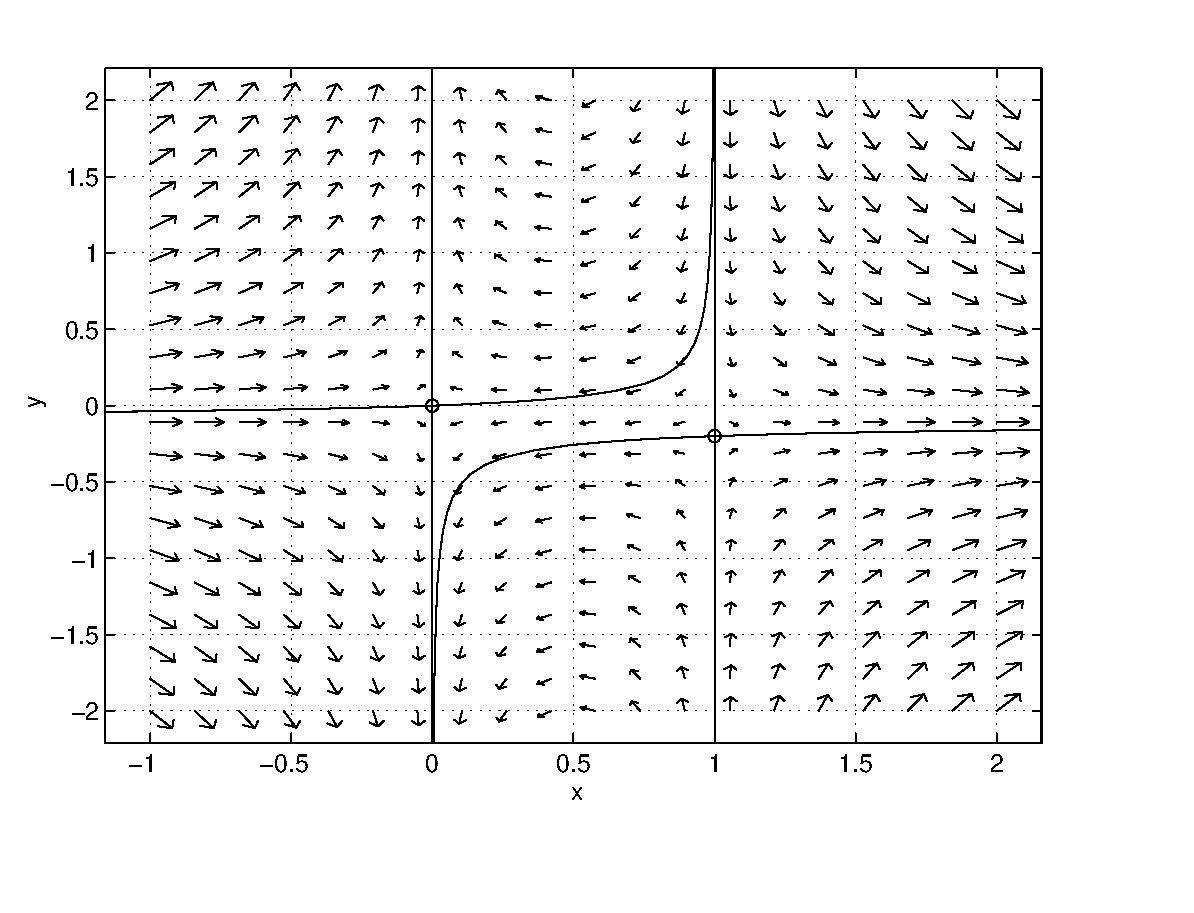
\psfig{file=figures/heteroa.eps,width=2.3in}
	   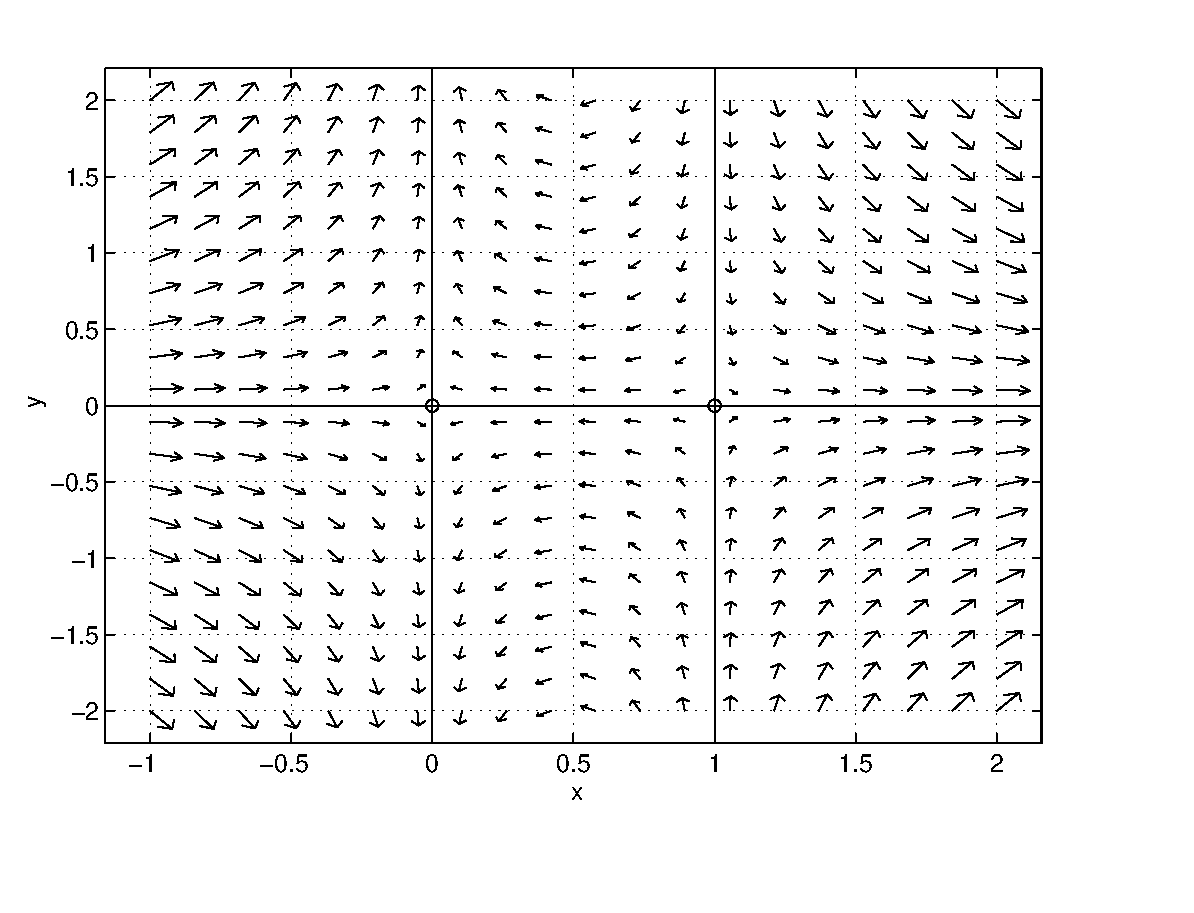
\psfig{file=figures/heterob.eps,width=2.3in}
	   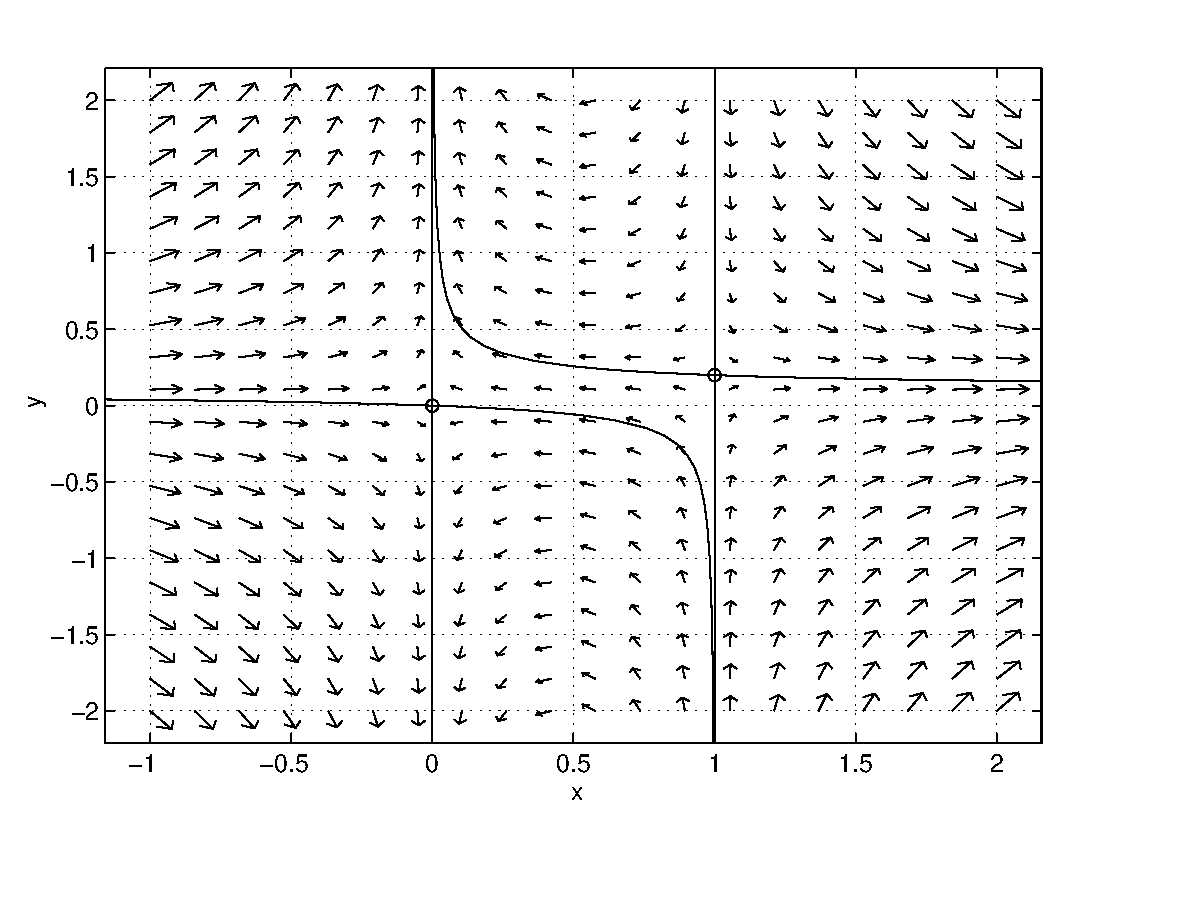
\psfig{file=figures/heteroc.eps,width=2.3in}}
 	\vspace*{-0.2in}
	\hspace{0.3in} $\rho=-0.1$  \hspace{1.7in} $\rho=0$
		\hspace{1.8in} $\rho=0.1$ 
           \caption{Phase portraits for \protect\Ref{e:hetero}. 
	Note the heteroclinic trajectory when $\rho=0$.}
           \label{F:hetero}
\end{figure}

\begin{figure}[htb]
           \centerline{%
	   \psfig{file=figures/heteroT.eps,width=2.5in}}
           \caption{Time series for heteroclinic trajectory 
		in \protect\Ref{e:hetero} when $\rho=0$.}
           \label{F:heteroT}
\end{figure}

When $\rho\neq 0$ the $x$-axis is no longer invariant for the differential 
equation.  The two saddles remain --- but there is no longer a 
trajectory connecting them.  In Figure~\ref{F:hetero} we use 
{\sf pplane5}\index{stable!orbit!in {\sf pplane5}} 
\index{unstable!orbit!in {\sf pplane5}}
to plot the stable and unstable orbits when $\rho=\pm 0.1$.

From this figure we can see how the stable orbit of the origin swings 
through the saddle at $(1,0)$ as the parameter $\rho$ is varied.  This
is typical of the way that a heteroclinic trajectory appears and disappears 
as a parameter is varied.  The fleeting existence of a heteroclinic trajectory
shows how the global fate of stable and unstable orbits emanating from a 
saddle point can change in a drastic fashion. 


\subsection*{A Classification of One Parameter Bifurcations}

The following is a complete list of expected transitions between planar 
Morse-Smale systems of different types in systems with one parameter.
\index{Morse-Smale system}
\begin{itemize}
\item	Two equilibria coalesce and disappear in a saddle-node bifurcation.
\index{bifurcation!saddle-node}
\item	A single equilibrium changes from a spiral source to a spiral sink (or 
vice-versa) and spawns a limit cycle in a Hopf bifurcation.
\index{bifurcation!Hopf}
\item	Two limit cycles coalesce in a saddle-node bifurcation of 
periodic solutions\index{bifurcation!saddle-node!of periodic solutions}.
\item	Stable and unstable orbits from distinct saddle points
coalesce and form a heteroclinic trajectory\index{trajectory!heteroclinic}.
\item	Limit cycles grow until they touch a saddle and form a homoclinic 
trajectory\index{trajectory!homoclinic}.
\end{itemize}


\EXER

\CEXER

\begin{exercise} \label{c9.5.1}
Use {\sf pplane5} to analyze the phase portraits for the system
\begin{equation*}
\begin{array}{rcl}
\dot{x} & = & (-\rho+3(0.5x^2+y^2)-(x^2+y^2)^2)x-2y \\
\dot{y} & = & (-\rho+3(x^2+y^2)-(1.3x^2+y^2)^2)y+x
\end{array}
\end{equation*}
for $\rho=0.7$ and $\rho=1.1$ on the square $-2\leq x,y\leq 2$.  Is there 
a bifurcation between these two values of $\rho$?  If so, what kind of 
bifurcation is it and what is the bifurcation value of $\rho$ to within 
$\pm 0.02$?
\end{exercise}

\noindent In Exercises~\ref{c9.6.2a} -- \ref{c9.6.2c}, consider the system 
of differential equations \Ref{E:homo2}
\begin{equation*}  \label{E:homo2}
\begin{array}{rcl}
\dot{x} & = & -y + \rho x + 0.1 x^2 - 0.5 y^5 \\
\dot{y} & = & x +\rho y + 0.1 y^3 - x^4
\end{array}
\end{equation*}
in the square $-1.5\leq x,y\leq 1.5$.
\begin{exercise} \label{c9.6.2a}
Verify numerically that \Ref{E:homo2} appears to have a limit cycle for 
$\rho=-0.02$.
\end{exercise} 
\begin{exercise} \label{c9.6.2b}
Verify numerically that \Ref{E:homo2} does not appear to have a limit cycle 
when $\rho=-0.03$.
\end{exercise} 
\begin{exercise} \label{c9.6.2c}
Determine numerically to two significant figures, the value of $\rho$
where \Ref{E:homo2} has a homoclinic bifurcation. 
\end{exercise} 

\noindent In Exercises~\ref{c9.6.3a} -- \ref{c9.6.3b}, consider the system 
of differential equations \Ref{E:infinity}.
\begin{equation*}  \label{E:infinity}
\begin{array}{rcl}
\dot{x} & = & y \\
\dot{y} & = & -x +\rho y + \frac{1}{2}\cos(x)y
\end{array}
\end{equation*}
\begin{exercise} \label{c9.6.3a}
How many periodic solutions does \Ref{E:infinity} appear to have 
when $\rho=0$?  Be careful when answering this question.  First use 
{\sf pplane5} to determine the number of limit cycles on the square 
$-\ell \leq x,y \leq\ell$ when $\ell=2$.  Then compute with $\ell=10$ and 
$\ell=40$.
\end{exercise}
\begin{exercise} \label{c9.6.3b}
Find the number of limit cycles to \Ref{E:infinity} on the square 
with $\ell=7$ when $\rho=0.06$ and when $\rho=0.07$.  Has a bifurcation
 occurred between these two values of $\rho$ and, if so, what kind of 
bifurcation?
\end{exercise}

\noindent In Exercises~\ref{c9.6.4a} -- \ref{c9.6.4c}, consider the system 
of differential equations \Ref{E:twoeq}
\begin{equation*}  \label{E:twoeq}
\begin{array}{rcl}
\dot{x} & = & y - x + (x-\rho)^2 \\
\dot{y} & = & y - x^3 +3x
\end{array}
\end{equation*}
in the square $-5 \leq x,y \leq 5$.
\begin{exercise} \label{c9.6.4a}
How many equilibria does \Ref{E:twoeq} have in this square when 
$\rho=1.7$ and of what type are they?  This question can be answered either 
numerically using {\sf pplane5} (easy) or analytically (more difficult, but 
possible).
\end{exercise}
\begin{exercise} \label{c9.6.4b}
What type of bifurcation occurs in \Ref{E:twoeq} as $\rho$ is varied
from $\rho=1.7$ to $\rho=1.85$?
\end{exercise}
\begin{exercise} \label{c9.6.4c}
What type of bifurcation occurs in \Ref{E:twoeq} as $\rho$ is varied
from $\rho=1.85$ to $\rho=2.1$?
\end{exercise}

\begin{exercise} \label{c9.6.6}
Embed system \Ref{c8.4.5a} of Chapter~\ref{C:NPS} in the family of systems of 
differential equations 
\begin{equation} \label{E:eqn2}
\begin{array}{rcl}
\dot{x} & = & \rho x-y-3y^2+2.5xy\\
\dot{y} & = & x-3x^2+2x^2y.
\end{array}
\end{equation}
Find seven bifurcations that occur in \Ref{E:eqn2} as $\rho$ varies from 
$-0.1$ to $\rho=0.3$. 
\end{exercise}

\noindent In Exercises~\ref{c9.6.5a} -- \ref{c9.6.5c}, consider the system 
of differential equations \Ref{E:saddleconn}.
\begin{equation*}  \label{E:saddleconn}
\begin{array}{rcl}
\dot{x} & = & y  \\
\dot{y} & = & -x - 0.1y + x^3 + \rho x^2.
\end{array}
\end{equation*}
\begin{exercise} \label{c9.6.5a}
How many equilibria does \Ref{E:saddleconn} have for each value of 
$\rho$ and of what type are they?  
\end{exercise}
\begin{exercise} \label{c9.6.5b}
How many bifurcations occur in \Ref{E:saddleconn} as $\rho$ is 
varied from $\rho=0.1$ to $\rho=0.2$?
\end{exercise}
\begin{exercise} \label{c9.6.5c}
What types of bifurcation occur in \Ref{E:saddleconn} as $\rho$ is 
varied from $\rho=0.1$ to $\rho=0.2$?
\end{exercise}



\Sec{*Saddle-Node Bifurcations Revisited}{SADDLE-NODE BIFURCATIONS REVISITED} 
\label{S:SNB}
\index{bifurcation!steady-state}  \index{bifurcation!saddle-node}


The simplest steady-state bifurcations --- and the ones that are most
likely to occur --- are the saddle-node bifurcations.  In 
Section~\ref{S:bifurcation} we found necessary conditions for the existence 
of saddle-node bifurcations in one dimension \Ref{E:DCSN} and two 
dimensions \Ref{E:DCSN2}.  In this section we describe necessary and 
sufficient conditions for the existence of saddle-node bifurcations.


\subsection*{Saddle-Node Bifurcation in One Dimension}

Consider the differential equation 
\begin{equation} \label{e:1dbif}
\dot{x} = f(x,\rho),
\end{equation}
that depends on the single parameter $\rho$.  The equilibria are 
found by solving the algebraic equation 
\begin{equation} \label{e:1dstst}
f(x,\rho) = 0.
\end{equation}
We can study how the equilibria in phase portraits for \Ref{e:1dbif} 
change when $\rho$ is varied by plotting
solutions to \Ref{e:1dstst} in the $\rho x$-plane.  The solutions to
\Ref{e:1dstst} form the bifurcation diagram of \Ref{e:1dbif}.

Recall from \Ref{E:DCSN} that  
\begin{equation}  \label{e:1dbifcond}
\begin{array}{rcl}
f(x_0,\rho_0) & = & 0 \\
f_x(x_0,\rho_0) & = & 0.
\end{array}
\end{equation}
are necessary conditions for a saddle-node bifurcation to occur at
$(x_0,\rho_0)$.  The simplest example of a saddle-node bifurcation is:
\begin{equation}  \label{e:1dsaddlenf}
f(x,\rho) = a x^2 + \rho,
\end{equation}
where $a$ is a nonzero constant.  The exact bifurcation diagram for 
\Ref{e:1dsaddlenf} depends on the sign of $a$.  See Figure~\ref{F:1dsaddle}.  
Note that the bifurcation diagram is just a parabola pointing either to the 
left or to the right.  The general saddle-node bifurcation is one whose 
bifurcation diagram looks `parabolic-like'.  Theorem~\ref{T:saddlenode}
makes this idea precise.

\begin{figure}[htb]
           \centerline{%
	   \psfig{file=figures/sbifBIF.eps,width=2.5in} \qquad \qquad
	   \psfig{file=figures/sbifBIF2.eps,width=2.5in}}
	 \hspace{1.0in} $a<0$ \hspace{2.8in}  $a>0$  
           \caption{Bifurcation diagrams for \protect\Ref{e:1dsaddlenf}.}
           \label{F:1dsaddle}
\end{figure}

\begin{thm}  \label{T:saddlenode} \index{bifurcation!saddle-node}
Suppose that the differential equation \Ref{e:1dbif} has an equilibrium
at $(x_0,\rho_0)$ satisfying the bifurcation conditions \Ref{e:1dbifcond}
and the nondegeneracy conditions\index{nondegeneracy conditions}
\begin{equation}  \label{e:nondegen1}
\begin{array}{rcl} 
f_\rho(x_0,\rho_0) & \neq & 0 \\
f_{xx}(x_0,\rho_0) & \neq & 0. 
\end{array}
\end{equation}
Then the bifurcation diagram $f=0$ looks like the diagram in 
Figure~\ref{F:1dsaddle} where 
\[
a = \frac{f_{xx}(x_0,\rho_0)}{f_\rho(x_0,\rho_0)}.
\]
\end{thm}

\proof  The proof of this theorem uses the implicit function theorem and
implicit differentiation.  (Technically, we need to assume that the second
derivatives of $f(x,\rho)$ are continuous before proceeding.) Since 
$f_\rho(x_0,\rho_0)$ is assumed to be nonzero, the implicit function theorem 
guarantees the existence of a function $R(x)$ such that $R(x_0)=\rho_0$ and
\begin{equation}  \label{e:implicit0}
f(x,R(x))\equiv 0
\end{equation}
for all $x$ near $x_0$.  It follows that the bifurcation diagram $f(x,\rho)=0$
is the graph $\rho = R(x)$.  We claim that $R'(x_0)=0$ and $R''(x_0)\neq 0$. 
Thus the Taylor series of the function $R(x)$ is
\[
R(x) = \rho_0 + \half R''(x_0)(x-x_0)^2 + \cdots 
\]
for all $x$ near $x_0$.  It follows that the bifurcation diagram $f=0$ is
parabolic in shape as in Figure~\ref{F:1dsaddle} --- opening either to the 
left or to the right depending on the sign of $R''(x_0)$.

We use implicit differentiation to verify these claims. Differentiating
\Ref{e:implicit0} twice yields 
\begin{equation}  \label{e:implicit1}
f_x(x,R(x)) + f_\rho(x,R(x))R'(x) \equiv 0,
\end{equation}
and 
\begin{equation}  \label{e:implicit2}
f_{xx}(x,R(x)) + 2f_{x\rho}(x,R(x))R'(x) + f_{\rho\rho}(x,R(x))R'(x)^2 
+ f_\rho(x,R(x))R''(x) \equiv 0.
\end{equation}

Evaluating \Ref{e:implicit1} at $x=x_0$ yields
\[
f_x(x_0,\rho_0) + f_\rho(x_0,\rho_0)R'(x_0) = 0. 
\]
Since, by assumption, $f_x(x_0,\rho_0)=0$ and $f_\rho(x_0,\rho_0)\neq 0$,
it follows that 
\[
R'(x_0)=0.
\]
Evaluating \Ref{e:implicit2} at $x=x_0$ now yields
\[
f_{xx}(x_0,\rho_0) +  f_\rho(x_0,\rho_0)R''(x_0) = 0
\]
The nondegeneracy assumptions \Ref{e:nondegen1} imply
\[
R''(x_0) = -\frac{f_{xx}(x_0,\rho_0)}{f_\rho(x_0,\rho_0)} \neq 0.
\]
Thus $a=-R''(x_0)$.  So when $R''(x_0)>0$ the number $a$ is negative and the
bifurcating branch is supercritical, as in Figure~\ref{F:1dsaddle}.  Similarly, 
when $R''(x_0)<0$ the number $a$ is positive and the bifurcating branch is 
subcritical. \qed
 
\subsubsection*{An Example of a One Dimensional Saddle-Node Bifurcation}

Consider the following example of a saddle-node bifurcation.  Let 
\begin{equation}  \label{e:sn1}
f(x,\rho) = -x^3 + 3x^2 - \rho x - 4.
\end{equation}
A quick check shows that $x=2$ is an equilibrium for \Ref{e:sn1} 
when $\rho=0$.  Moreover, 
\[
f(2,0)=0, \quad f_x(2,0)=0, \quad f_\rho(2,0)=-2\neq 0, 
\quad f_{xx}(2,0)=-6\neq 0.
\]
It follows from Theorem~\ref{T:saddlenode} that $f$ has a saddle-node
bifurcation when $\rho=0$ at $x=2$.  Indeed, since $a=\frac{-6}{-2}=3>0$, 
it follows that there are two equilibria near $x=2$ when $\rho<0$ and 
none when $\rho>0$.  See Figure~\ref{F:1dsaddle}. This fact can be 
verified using {\sf pline}.  When $\rho$ is small and positive, there is 
one stable equilibrium near $x=-1$.  When $\rho$ is small and negative, there 
are three equilibria --- the stable one near $x=-1$ and two new equilibria 
near $x=2$ formed from the saddle-node bifurcation.  



\subsection*{Saddle-Node Bifurcations in Two Dimensions}
\index{bifurcation!saddle-node}

In higher dimensions, steady-state bifurcations occur at parameter 
values where the Jacobian matrix\index{matrix!Jacobian}
has a zero eigenvalue.  In one dimension,
the $1\times 1$ Jacobian matrix is the number $f_x$.  Such a 
Jacobian matrix has a zero eigenvalue precisely when $f_x$ vanishes
--- which is just the condition in \Ref{e:1dbifcond}.  

In two dimensions, the Jacobian matrix $J$ is a saddle-node matrix when
it has a single zero eigenvalue, that is, when $\det(J)=0$ and 
$\trace(J)\neq 0$.  Now consider the planar system of differential equations 
depending on a parameter $\rho$.  We write this system as
\begin{equation}  \label{e:2deqn}
\dot{X} = F(X,\rho),
\end{equation}
where $X=(x,y)\in\R^2$ and $F=(g,h)$ in coordinates.  Sufficient conditions
for the existence of a saddle-node bifurcation in \Ref{e:2deqn} are as follows.
\begin{enumerate}
\item Equation~\Ref{e:2deqn} has an equilibrium at $(X_0,\rho_0)$; so 
\[
F(X_0,\rho_0) = 0.
\]
\item  The Jacobian matrix 
\[
J=(dF)_{(X_0,\rho_0)}=
\mattwo{g_x(X_0,\rho_0)}{g_y(X_0,\rho_0)}{h_x(X_0,\rho_0)}{h_y(X_0,\rho_0)}.
\]
has a zero eigenvalue and a nonzero eigenvalue.  Let $w$ be a nonzero vector 
in the null space of $J^t$.  Assume
\begin{equation}  \label{e:2deig}
w \cdot F_\rho(X_0,\rho_0) \neq 0,
\end{equation}
where $F_\rho=(g_\rho,h_\rho)$.  (In one dimension, \Ref{e:2deig} just states 
that $f_\rho(X_0,\rho_0)$ is nonzero; that is, the first
nondegeneracy condition\index{nondegeneracy conditions} in 
\Ref{e:nondegen1} is valid.) 
\item   Let $v=(v_1,v_2)$ be a nonzero vector in the null space of $J$.
The following is an analogue in two dimensions for the second nondegeneracy
condition in \Ref{e:nondegen1}, $f_{xx}(x_0,\rho_0)\neq 0$. Define $F_0$ to 
be the vector
\[
F_0 = v_1^2\vectwo{g_{xx}}{h_{xx}} + 2v_1v_2\vectwo{g_{xy}}{h_{xy}}
+ v_2^2 \vectwo{g_{yy}}{h_{yy}}  
\]
evaluated at $(X_0,\rho_0)$.  The nondegeneracy condition in two dimensions
is:
\begin{equation}  \label{e:2dbifur}
w \cdot F_0 \neq 0.
\end{equation}
\end{enumerate}
A steady-state bifurcation is a {\em saddle-node bifurcation\/} if 
\Ref{e:2deig} and \Ref{e:2dbifur} are valid.  At a saddle-node bifurcation 
two equilibria coalesce as $\rho$ is varied, and the bifurcation diagram 
resembles that in Figure~\ref{F:1dsaddle}.

\subsubsection*{An Example of a Two Dimensional Saddle-Node Bifurcation}

As an example, consider the system of differential equations
\begin{equation*}  \label{e:snex}
\begin{array}{rcccl}
\dot{x} & = & \rho + x + 3y -xy & \equiv & g(x,y) \\
\dot{y} & = & -\rho + 2x + 6y + 3x^2 & \equiv & h(x,y).  
\end{array}
\end{equation*}
At $\rho = 0$, \Ref{e:snex} has an equilibrium at the origin with 
Jacobian matrix
\[
J = \mattwo{1}{3}{2}{6}.
\]
Since $\det(J)=0$, the origin is a bifurcation point.  Define the 
vectors $v$ and $w$ by
\[
Jv=0 \AND J^tw=0.
\]
So
\[
v = \vectwo{3}{-1} \AND  w = \vectwo{2}{-1}.
\]
Next compute
\[
F_\rho = \vectwo{1}{-1}.
\]
Therefore
\[
w \cdot F_\rho = \vectwo{2}{-1} \cdot \vectwo{1}{-1} = 3 \neq 0,
\]
and \Ref{e:2deig} is satisfied.  

Next compute
\[
g_{xx}=0, \quad g_{xy}=-1, \quad g_{yy}=0, \quad
h_{xx}=6, \quad h_{xy}=0, \quad h_{yy} = 0.
\]
Hence
\[
F_0 = v_1^2 \vectwo{0}{6} + 2v_1v_2\vectwo{-1}{0} = \vectwo{6}{54},
\]
and 
\[
w\cdot F_0 = \vectwo{2}{-1} \cdot \vectwo{6}{54} = -42 \neq 0.
\]
So \Ref{e:2dbifur} is satisfied. These conditions show that there is
a saddle-node bifurcation at the origin and that two equilibria 
coalesce as $\rho$ varies through zero. 

Some experimentation will convince you that it is complicated to find 
a closed form analytic solution for the equilibria of \Ref{e:snex}.  
We can, however, verify the existence of a saddle-node bifurcation 
using {\sf pplane5}.  The phase plane portraits are shown in 
Figure~\ref{F:snex}.

\begin{figure}[htb]
           \centerline{%
	   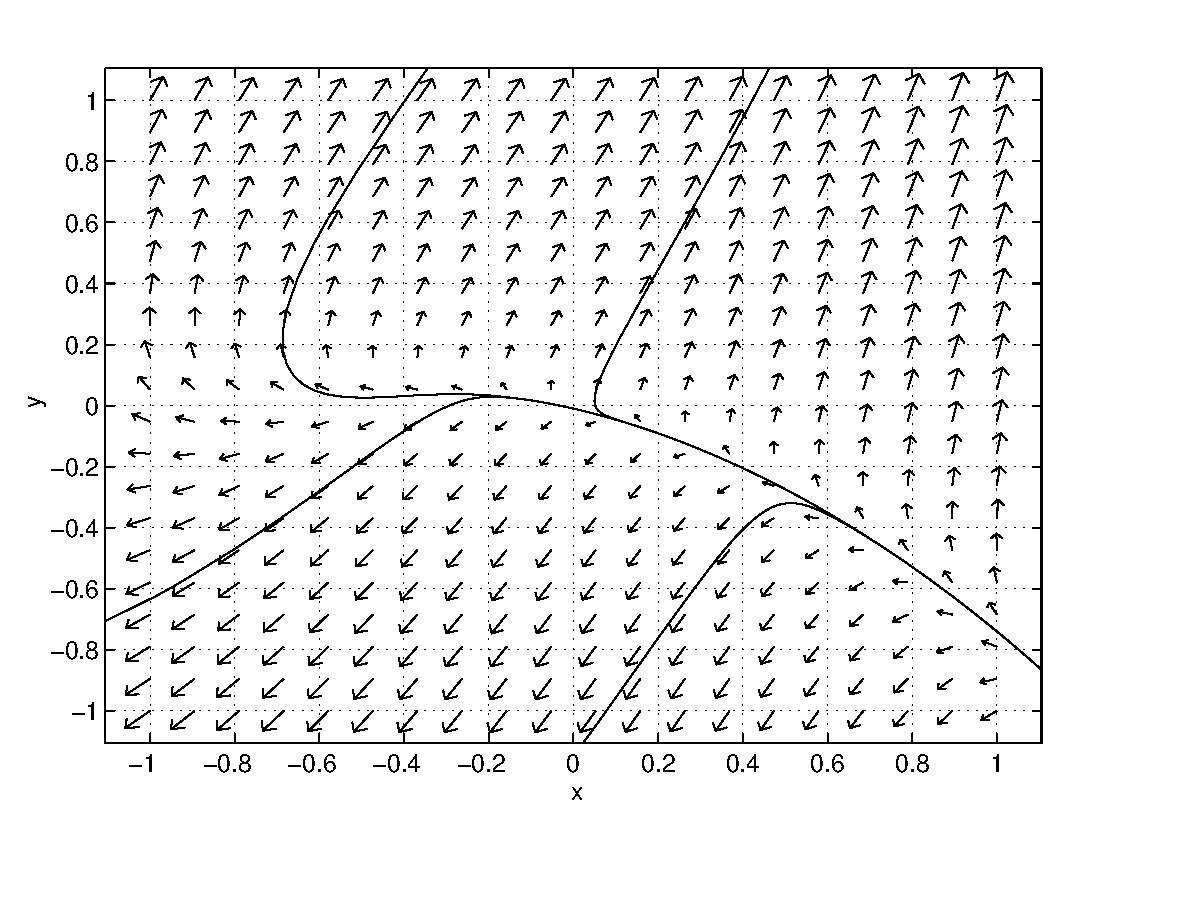
\psfig{file=figures/snexa.eps,width=3.2in}
	   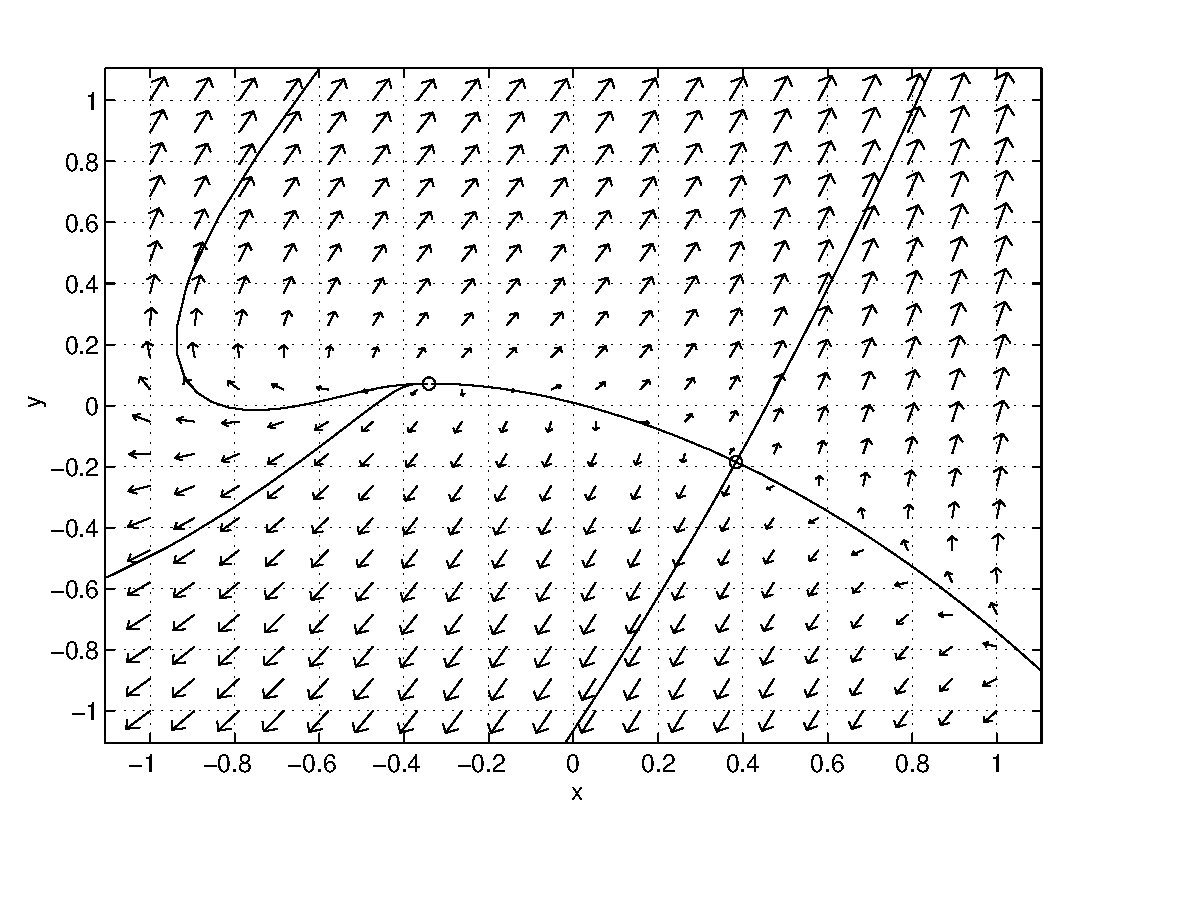
\psfig{file=figures/snexb.eps,width=3.2in}}
	\vspace*{-0.2in}
	\hspace{1.0in} $\rho=-0.1$  \hspace{2.55in} $\rho=0.1$ 
           \caption{Phase plane portrait for \protect\Ref{e:snex} on 
	the square $-1\leq x,y \leq 1$.  Note that there are no 
	equilibria when $\rho=-0.1$ and two equilibria when $\rho=0.1$.}
           \label{F:snex}
\end{figure}


\EXER

\TEXER

\begin{exercise} \label{c9.3.1}
Let 
\begin{eqnarray*}
f_1(x,\rho) & = & \rho - x^3 \\
f_2(x,\rho) & = & \rho x - x^2.
\end{eqnarray*}
\begin{itemize}
\item[(a)] Verify that both $f_1$ and $f_2$ satisfy the bifurcation conditions 
\Ref{e:1dbifcond} at $x=0$ when $\rho=0$.
\item[(b)] Show that neither $f_1$ nor $f_2$ has a saddle-node bifurcation
at $x=0$ when $\rho=0$. 
\item[(c)] Draw the bifurcation diagrams $f_1(x,\rho)=0$ and 
$f_2(x,\rho)=0$ and explain why the conclusion of 
Theorem~\ref{T:saddlenode} is not satisfied for either $f_1$ 
or $f_2$.
\end{itemize}
\end{exercise}

\begin{exercise} \label{c9.3.5}
Find all saddle-node bifurcations in the 
family of differential equations
\begin{equation}
\dot{x} = x^3 -5x^2 + 3x + \rho
\end{equation}
analytically.  Draw the bifurcation diagram.
\end{exercise}

\begin{exercise} \label{c9.3.2}
Let 
\[
f(x,\rho) = x^4 - 6x^3 +8x^2 + 6(x-\rho) - 3.
\]
Show that $f$ has a saddle-node bifurcation at $x=3$ when $\rho=1$. 
Are there two equilibria near $x=3$ when $\rho<1$ or when $\rho>1$?
\end{exercise}

\begin{exercise} \label{c9.3.3}
Let 
\begin{eqnarray*}
g(x,y,\rho) & = &  \rho - 2x +  y + 2x^2 - y^3 \\
h(x,y,\rho) & = & 2\rho + 4x - 2y -  xy  + y^2
\end{eqnarray*}
Show that $F=(g,h)$ has a saddle-node bifurcation at $(x,y)=0$ and 
$\rho=0$.
\end{exercise}


\begin{exercise} \label{c9.3.4}
Let $X=(x,y)$ and 
\[
F(X,\rho) = \rho q + \mattwo{1}{0}{0}{0} X + Q(X)
\]
where
\[
q=\vectwo{q_1}{q_2} \AND Q(X) = \vectwo{\alpha x^2+\beta xy+\gamma y^2}
{\delta x^2 +\epsilon xy+\varphi y^2}.
\]
Show that $F$ has a saddle-node bifurcation at $X=0$ and $\rho=0$ precisely 
when $q_2\neq 0$ and $\varphi\neq 0$. 
\end{exercise}



\Sec{*Hopf Bifurcations Revisited}{HOPF BIFURCATIONS REVISITED}  
\label{S:HopfBif}
\index{bifurcation!Hopf}

As discussed in Section~\ref{S:bifurcation}, Hopf bifurcation occurs at
an equilibrium when the Jacobian $J$ has a pair of complex conjugate, purely 
imaginary eigenvalues, that is, when $\trace(J)=0$ and $\det(J)>0$.  In two 
dimensions, $J$ is a center and the phase portrait of the linearized equation 
consists of a continuous family of periodic solutions.  The Hopf bifurcation 
theorem states that under reasonable assumptions this family of periodic 
solutions persists in the nonlinear equations.   \index{periodic solution}

Since $J$ is invertible, the (two dimensional) implicit function theorem 
guarantees that there is a curve of equilibria with one equilibrium for 
each value $\rho$ near the bifurcation value.  Because of this, it makes 
sense to ask how the real parts of the eigenvalues of the Jacobian are 
changing as $\rho$ varies.  The basic assumption that we make about Hopf 
bifurcation is that the real parts of the eigenvalues of the Jacobian go 
through zero with nonzero speed.  We can rewrite this condition algebraically 
as follows.  Let $X(\rho)$ denote the curve of equilibria and $J_{X(\rho)}$ 
the corresponding Jacobian matrix.  Then, the real part of the complex 
conjugate eigenvalues of the Jacobian matrix is: 
\index{eigenvalue crossing condition}
\[
\frac{1}{2}\trace(J_{X(\rho)}). 
\]
The condition that the real parts of the eigenvalues cross through 
zero with nonzero speed is:
\begin{equation}  \label{e:2dhopf}
\frac{d}{d\rho} \trace(J_{X(\rho)}) \neq 0.
\end{equation}
Condition \Ref{e:2dhopf} is called the {\em eigenvalue crossing condition\/}.


\subsection*{Two Examples}

As a first example, consider the linear system
\begin{equation*}  \label{e:Hopflin}
\begin{array}{rcl}
\dot{x} & = & \rho x - y \\
\dot{y} & = & x + \rho y.
\end{array}
\end{equation*}
It is easy to check that $\trace(J)=2\rho$ and that \Ref{e:2dhopf}
is satisfied.  Note that the origin is a spiral sink when $\rho<0$ 
and a spiral source when $\rho>0$.  When $\rho=0$, the origin is a
center, and there is a continuous family of periodic solutions
surrounding this center.  See Figure~\ref{F:Hopfabc}

\begin{figure}[htb]
           \centerline{%
           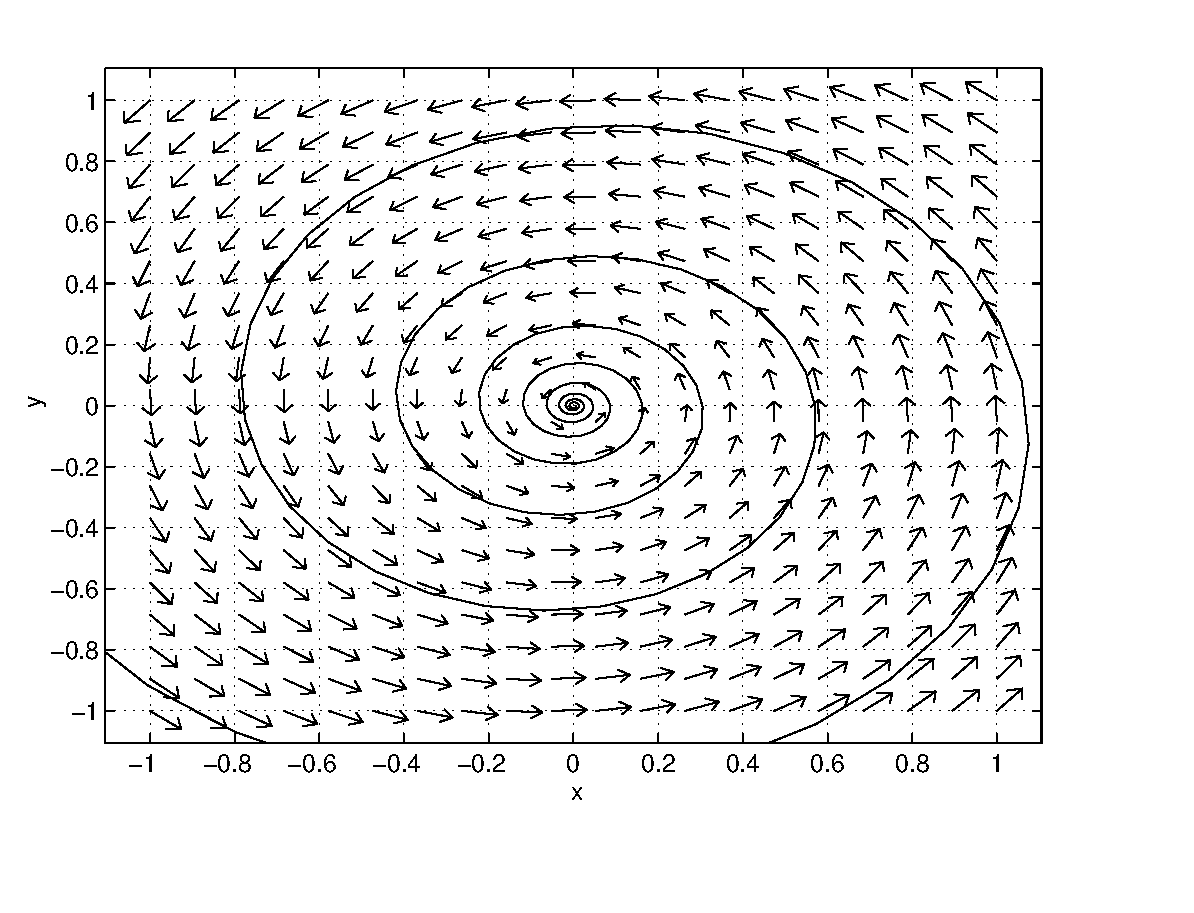
\psfig{file=figures/hopfa.eps,width=2.3in}
           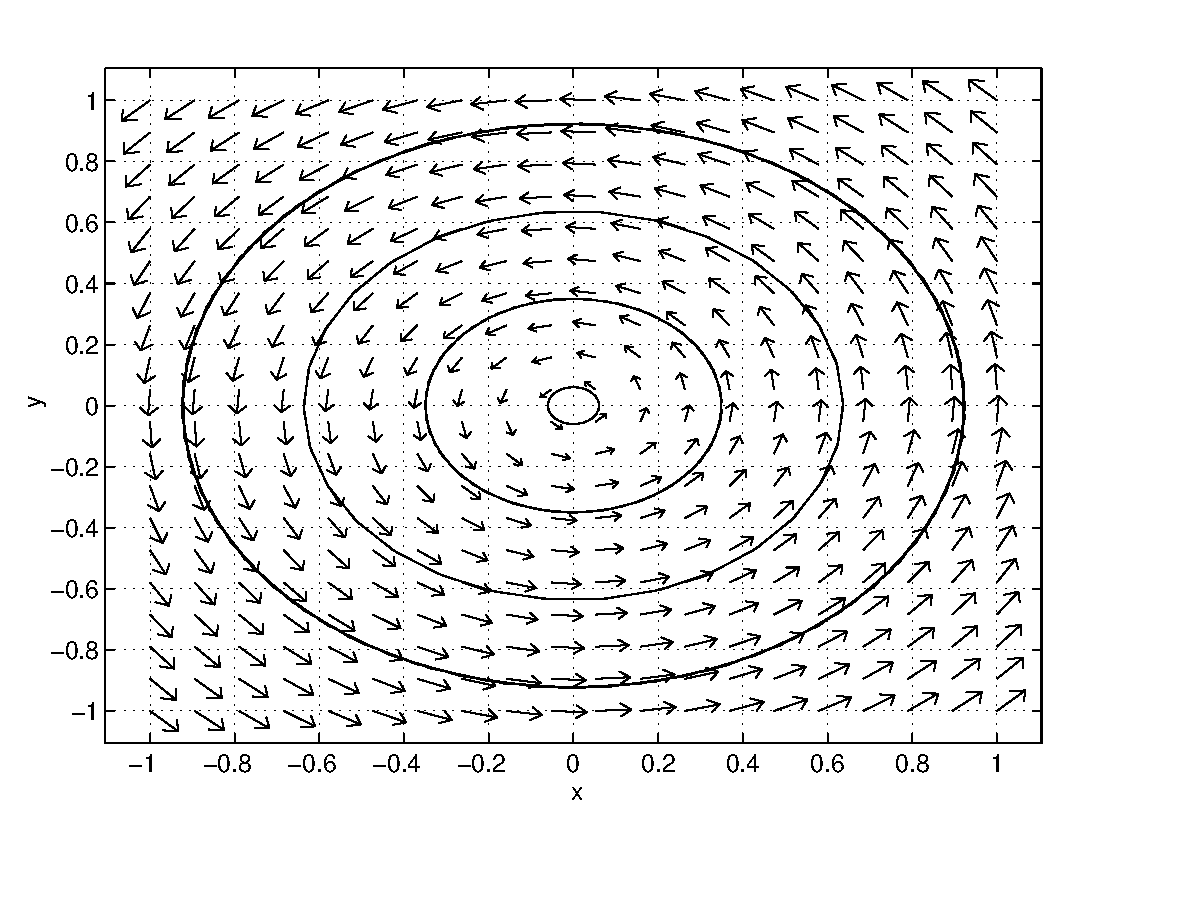
\psfig{file=figures/hopfb.eps,width=2.3in} 
           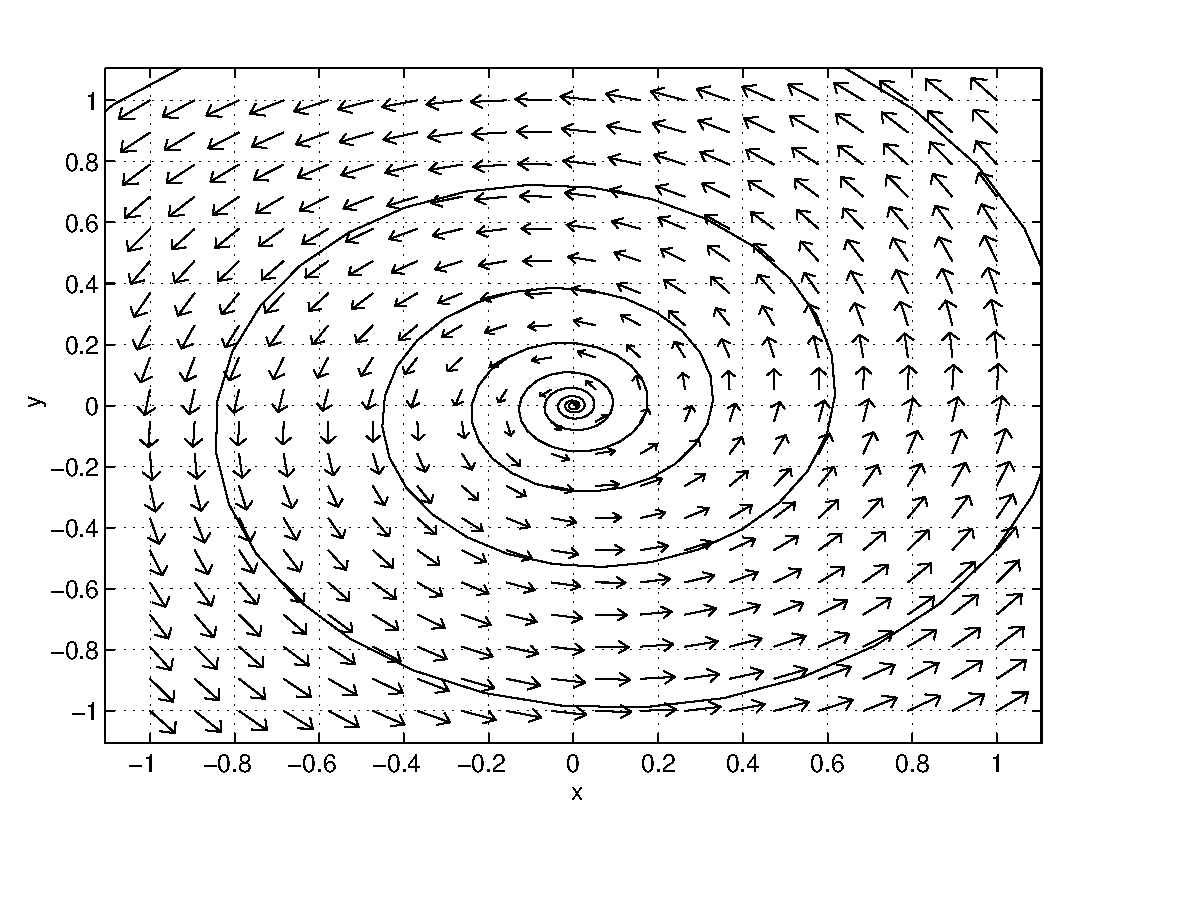
\psfig{file=figures/hopfc.eps,width=2.3in}}
	\vspace*{-0.2in}
	\hspace{0.3in} $\rho=-0.1$  \hspace{1.7in} $\rho=0$
		\hspace{1.8in} $\rho=0.1$ 
           \caption{Phase planes for \protect\Ref{e:Hopflin}.}
           \label{F:Hopfabc}
\end{figure}


As a second example, consider the predator-prey Volterra-Lotka 
equations \Ref{e:pop3}.  These equations are: \index{Volterra-Lotka equations}
\begin{equation} \label{e:pop3a}
\begin{array}{rcl}
\dot{x} & = & x(\mu + \rho x -       y) \\
\dot{y} & = & y( -1 +       x).
\end{array}
\end{equation}   
We fix $\mu>0$ and vary the parameter $\rho$.  Our previous 
calculations showed that \Ref{e:pop3a} has a center when 
$\rho=0$.  Indeed, these equations have a nontrivial equilibrium 
at $(x_0,y_0)=(1, \mu+\rho)$.  So $X(\rho)=(1,\mu+\rho)$.

The Jacobian matrix of \Ref{e:pop3a} is
\[
J_{(x,y)} = \left(\begin{array}{cc} \mu + 2\rho x - y & -x \\
y & -1 + x \end{array}\right).
\]
Evaluating $J$ along the equilibria $X(\rho)$ yields
\[
J_{(1,\mu+\rho)} = \left(\begin{array}{cc} \rho & -1 \\
\mu+\rho & 0 \end{array}\right).
\]
It follows that
\[
\trace(J_{X(\rho)}) = \rho,
\]
and hence 
\[
\frac{d}{d\rho} \trace(J_{X(\rho)}) = 1 \neq 0.
\]
So the eigenvalue crossing condition is satisfied for equation 
\Ref{e:pop3a}.  

\begin{thm}[simple Hopf bifurcation]  \label{T:2dhopf}
Suppose that the system of differential equations \Ref{e:2deqn}
has a point of Hopf bifurcation at $(X_0,\rho_0)$.  Suppose, in 
addition, that the 
eigenvalue crossing\index{eigenvalue crossing condition} 
condition \Ref{e:2dhopf} 
is satisfied.  Then there exists a unique branch of periodic 
solutions to \Ref{e:2deqn} emanating from $(X_0,\rho_0)$. 

Moreover, every periodic solution to \Ref{e:2deqn} that occurs for
a parameter value $\rho$ near $\rho_0$ and in phase space near $X_0$ 
is included in this branch of periodic solutions.
\end{thm}  \index{bifurcation!Hopf}

Recall that the predator-prey equations are obtained from \Ref{e:pop3a}
by setting $\rho=0$.  We have seen in our numerical analysis of the 
predator-prey equations that for all values of $\mu>0$ there is a center 
surrounded by a continuous family of periodic solutions.  (We 
have not proved this fact, but it is true.)  Since the eigenvalue 
crossing condition is satisfied for the predator-prey Volterra-Lotka 
equations, it follows from the simple Hopf bifurcation theorem that 
there are no other periodic solutions near the bifurcation point. 
\index{predator-prey equation}  Indeed, the numerical computations 
shown in Figure~\ref{F:pop3} support this conclusion.

\subsection*{A Significant Effect of Nonlinearity}

The most important point about the periodic solutions guaranteed by 
Theorem~\ref{T:2dhopf} is that they need not occur at the same parameter 
value. For example, in the CSTR there is an isolated limit cycle for each 
value of $\rho$ on one side of the bifurcation value.  See the numerical 
calculations of the CSTR in Figure~\ref{F:CSTR} for $\rho=0.545$ where an
isolated limit cycle is observed, and $\rho=0.520$ where no periodic
solution is seen. \index{CSTR}

Indeed, the CSTR equations behave more typically than the 
Volterra-Lotka equations.  What we expect to happen at a Hopf bifurcation 
point is summarized by the bifurcation diagrams of Figures~\ref{F:hopf} and 
\ref{F:hopf2}.  In these figures we see a single branch of periodic solutions 
emanating from the Hopf bifurcation point either 
{\em supercritically\/}\index{bifurcation!supercritical} (for 
values of $\rho$ greater than the one where Hopf bifurcation occurs) or 
{\em subcritically\/}\index{bifurcation!subcritical} 
(for values of $\rho$ less than the critical Hopf bifurcation value).

\begin{figure}[htb]
           \centerline{%
	   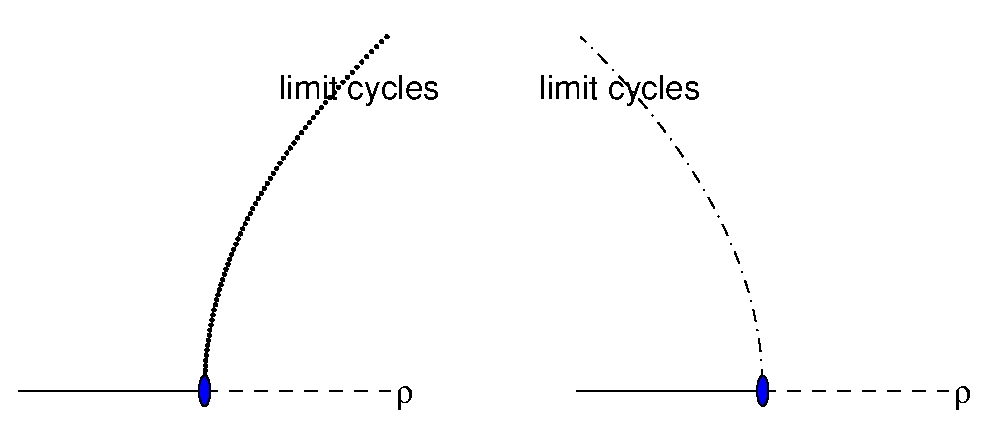
\psfig{file=figures/Hopfbif1a.eps,height=1.7in}}
           \caption{Typical bifurcation diagrams for Hopf bifurcation.}
           \label{F:hopf}
\end{figure}

\begin{figure}[htb]
           \centerline{%
	   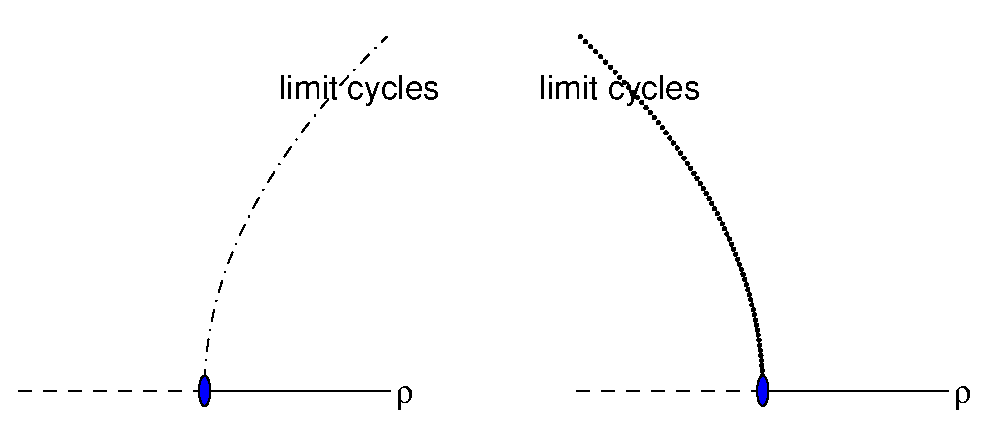
\psfig{file=figures/Hopfbif1b.eps,height=1.7in}}
           \caption{Typical bifurcation diagrams for Hopf bifurcation.}
           \label{F:hopf2}
\end{figure}

\subsubsection*{Exchange of Stability}
\index{stability!exchange of}

Assume that the equilibrium solution is stable at values below the 
bifurcation value and that the eigenvalue crossing condition \Ref{e:2dhopf} 
holds.  Then typically the periodic solutions will appear above 
the bifurcation value and be asymptotically 
stable\index{stability!asymptotic} or they will 
appear below the bifurcation value and be unstable.  Which one of these 
scenarios actually occurs depends on the sign of a certain coefficient 
computed from the second and third order terms of the differential equation.  
This coefficient plays the same role in Hopf bifurcation that condition 
\Ref{e:2dbifur} plays in saddle-node bifurcations.  The coefficient is 
much more complicated than \Ref{e:2dbifur} and we do not attempt to give 
its explicit form here.

If, on the other hand, the equilibrium solution is unstable at values below 
the bifurcation value, then the periodic solutions will be unstable when
supercritical and stable when subcritical.  See Figure~\ref{F:hopf2}.  In 
particular, the periodic solutions are stable only when they appear on the 
opposite side of criticality from the stable equilibrium.  This phenomenon 
is called {\em exchange of stability\/}.

\subsubsection*{Hopf Bifurcation in Phase-Amplitude Equations}

We can understand how typical Hopf bifurcations behave by looking at
phase-ampli\-tude equations of ODEs. The system is:  
\index{phase-amplitude equations}
\begin{equation*}  \label{e:nonlinhopf}
\frac{d}{dt}\vectwo{x}{y} = (\rho +a(x^2+y^2))\vectwo{x}{y} + \vectwo{-y}{x}.
\end{equation*}
In amplitude $r$ and phase $\theta$, \Ref{e:nonlinhopf} becomes
\begin{eqnarray*}
\dot{r} & = & (\rho+ar^2)r \\
\dot{\theta} & = & 1.
\end{eqnarray*}
The nontrivial zeros of the amplitude equation --- which correspond to 
periodic solutions in the original system --- are 
\[
\rho = -a r^2.
\]
It follows that there is one periodic trajectory of \Ref{e:nonlinhopf}
for $\rho>0$ when $a<0$ and for $\rho<0$ when $a>0$.  
Phase portraits for \Ref{e:nonlinhopf} when $a=-1$ are presented in 
Figure~\ref{F:nonlinhopf}.  Note the existence of a stable limit 
cycle\index{limit cycle!stable}
when $\rho>0$ and the slowness of the convergence of trajectories 
to the origin when $\rho=0$.

\begin{figure}[htb]
           \centerline{%
           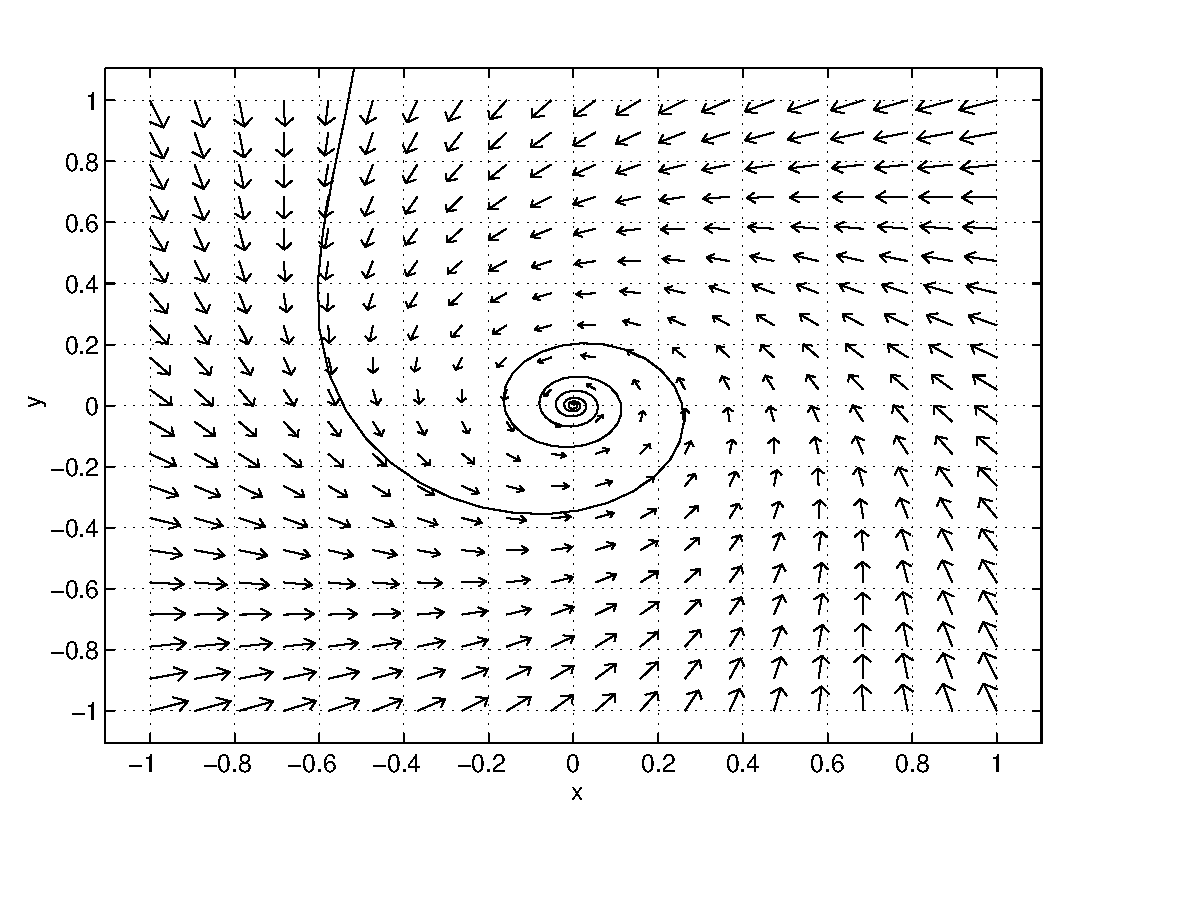
\psfig{file=figures/hopfna.eps,width=2.3in}
           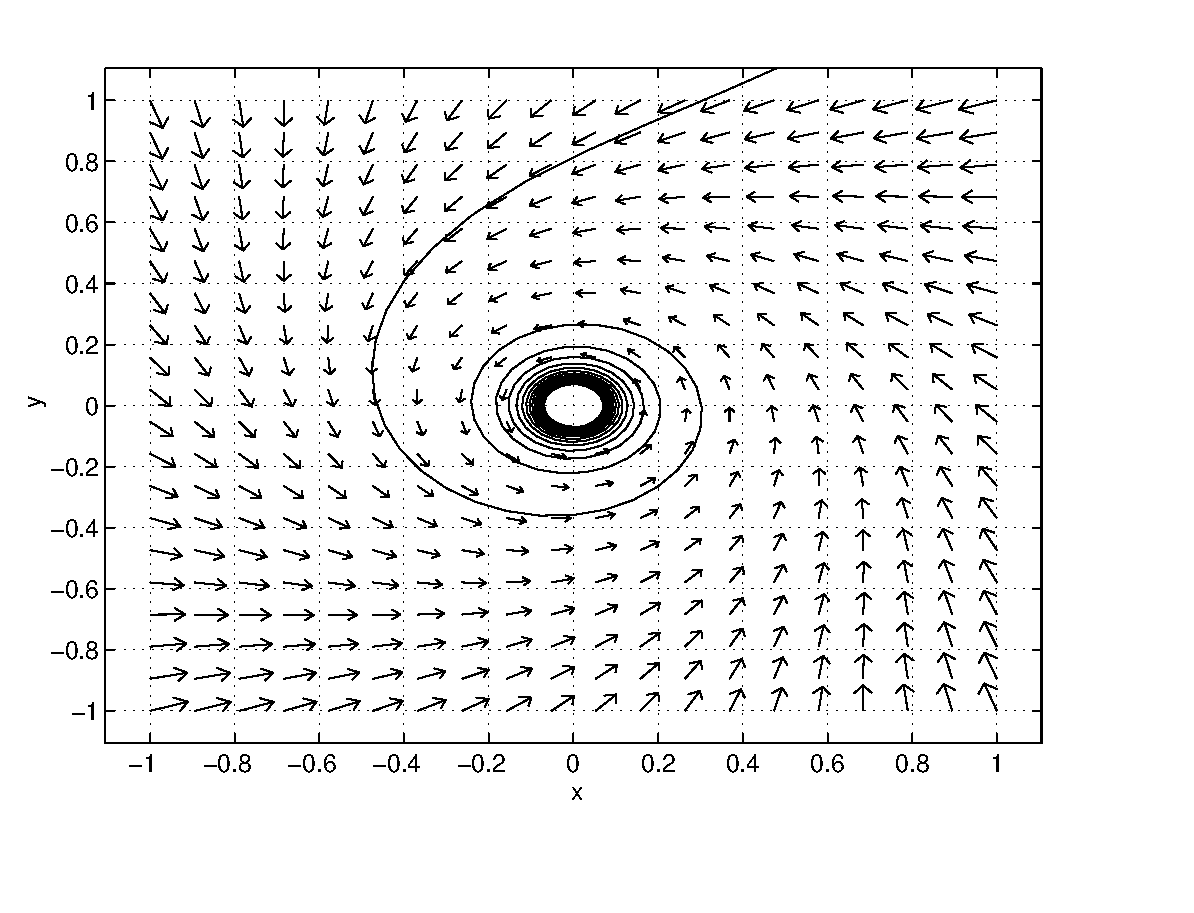
\psfig{file=figures/hopfnb.eps,width=2.3in} 
           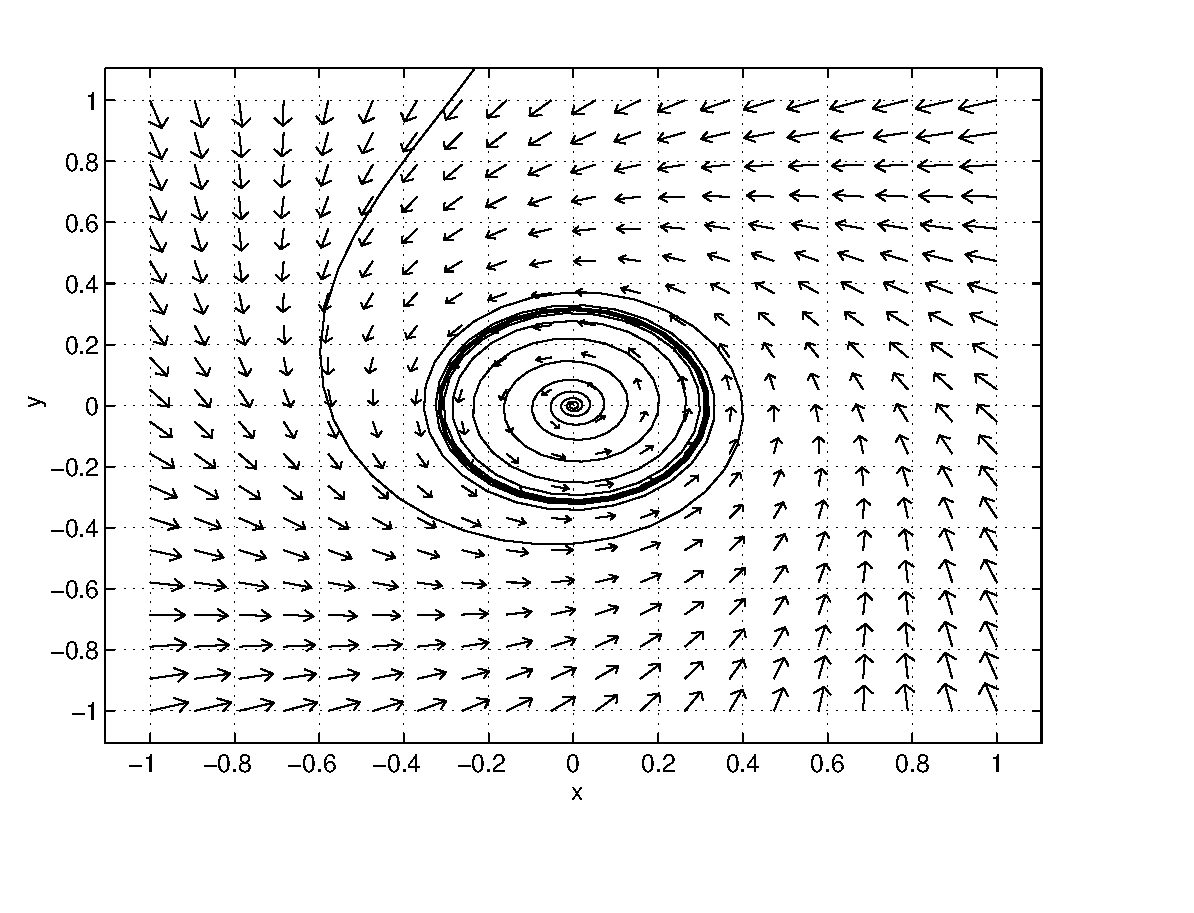
\psfig{file=figures/hopfnc.eps,width=2.3in}}
 	\vspace*{-0.2in}
	\hspace{0.3in} $\rho=-0.1$  \hspace{1.7in} $\rho=0$
		\hspace{1.8in} $\rho=0.1$ 
          \caption{Phase planes for \protect\Ref{e:nonlinhopf} with $a=-1$.}
           \label{F:nonlinhopf}
\end{figure}



\EXER

\TEXER

\noindent In Exercises~\ref{c9.6.1a} -- \ref{c9.6.1b} find points of Hopf
bifurcation and check for these points whether the eigenvalue crossing
condition \Ref{e:2dhopf} is satisfied.
\begin{exercise} \label{c9.6.1a}
$\begin{array}{rcl}
\dot{x} & = & \rho x - y -x^3 \\
\dot{y} & = & x.
\end{array}$
\end{exercise}
\begin{exercise} \label{c9.6.1b}
$\begin{array}{rcl}
\dot{x} & = & y - \rho x - x^2   \\
\dot{y} & = & -x - \rho y + x^2.
\end{array}$
\end{exercise}


































